% Options for packages loaded elsewhere
\PassOptionsToPackage{unicode}{hyperref}
\PassOptionsToPackage{hyphens}{url}
\PassOptionsToPackage{dvipsnames,svgnames,x11names}{xcolor}
\documentclass[
]{article}
\usepackage{xcolor}
\usepackage[margin=0.42in]{geometry}
\usepackage{amsmath,amssymb}
\setcounter{secnumdepth}{5}
\usepackage{iftex}
\ifPDFTeX
  \usepackage[T1]{fontenc}
  \usepackage[utf8]{inputenc}
  \usepackage{textcomp} % provide euro and other symbols
\else % if luatex or xetex
  \usepackage{unicode-math} % this also loads fontspec
  \defaultfontfeatures{Scale=MatchLowercase}
  \defaultfontfeatures[\rmfamily]{Ligatures=TeX,Scale=1}
\fi
\usepackage{lmodern}
\ifPDFTeX\else
  % xetex/luatex font selection
\fi
% Use upquote if available, for straight quotes in verbatim environments
\IfFileExists{upquote.sty}{\usepackage{upquote}}{}
\IfFileExists{microtype.sty}{% use microtype if available
  \usepackage[]{microtype}
  \UseMicrotypeSet[protrusion]{basicmath} % disable protrusion for tt fonts
}{}
\makeatletter
\@ifundefined{KOMAClassName}{% if non-KOMA class
  \IfFileExists{parskip.sty}{%
    \usepackage{parskip}
  }{% else
    \setlength{\parindent}{0pt}
    \setlength{\parskip}{6pt plus 2pt minus 1pt}}
}{% if KOMA class
  \KOMAoptions{parskip=half}}
\makeatother
\usepackage{longtable,booktabs,array}
\newcounter{none} % for unnumbered tables
\usepackage{calc} % for calculating minipage widths
% Correct order of tables after \paragraph or \subparagraph
\usepackage{etoolbox}
\makeatletter
\patchcmd\longtable{\par}{\if@noskipsec\mbox{}\fi\par}{}{}
\makeatother
% Allow footnotes in longtable head/foot
\IfFileExists{footnotehyper.sty}{\usepackage{footnotehyper}}{\usepackage{footnote}}
\makesavenoteenv{longtable}
\usepackage{graphicx}
\makeatletter
\newsavebox\pandoc@box
\newcommand*\pandocbounded[1]{% scales image to fit in text height/width
  \sbox\pandoc@box{#1}%
  \Gscale@div\@tempa{\textheight}{\dimexpr\ht\pandoc@box+\dp\pandoc@box\relax}%
  \Gscale@div\@tempb{\linewidth}{\wd\pandoc@box}%
  \ifdim\@tempb\p@<\@tempa\p@\let\@tempa\@tempb\fi% select the smaller of both
  \ifdim\@tempa\p@<\p@\scalebox{\@tempa}{\usebox\pandoc@box}%
  \else\usebox{\pandoc@box}%
  \fi%
}
% Set default figure placement to htbp
\def\fps@figure{htbp}
\makeatother
% definitions for citeproc citations
\NewDocumentCommand\citeproctext{}{}
\NewDocumentCommand\citeproc{mm}{%
  \begingroup\def\citeproctext{#2}\cite{#1}\endgroup}
\makeatletter
 % allow citations to break across lines
 \let\@cite@ofmt\@firstofone
 % avoid brackets around text for \cite:
 \def\@biblabel#1{}
 \def\@cite#1#2{{#1\if@tempswa , #2\fi}}
\makeatother
\newlength{\cslhangindent}
\setlength{\cslhangindent}{1.5em}
\newlength{\csllabelwidth}
\setlength{\csllabelwidth}{3em}
\newenvironment{CSLReferences}[2] % #1 hanging-indent, #2 entry-spacing
 {\begin{list}{}{%
  \setlength{\itemindent}{0pt}
  \setlength{\leftmargin}{0pt}
  \setlength{\parsep}{0pt}
  % turn on hanging indent if param 1 is 1
  \ifodd #1
   \setlength{\leftmargin}{\cslhangindent}
   \setlength{\itemindent}{-1\cslhangindent}
  \fi
  % set entry spacing
  \setlength{\itemsep}{#2\baselineskip}}}
 {\end{list}}
\usepackage{calc}
\newcommand{\CSLBlock}[1]{\hfill\break\parbox[t]{\linewidth}{\strut\ignorespaces#1\strut}}
\newcommand{\CSLLeftMargin}[1]{\parbox[t]{\csllabelwidth}{\strut#1\strut}}
\newcommand{\CSLRightInline}[1]{\parbox[t]{\linewidth - \csllabelwidth}{\strut#1\strut}}
\newcommand{\CSLIndent}[1]{\hspace{\cslhangindent}#1}
\setlength{\emergencystretch}{3em} % prevent overfull lines
\providecommand{\tightlist}{%
  \setlength{\itemsep}{0pt}\setlength{\parskip}{0pt}}
% Standalone-render preamble: load the same packages the template's
% manuscript/preamble.md declares (siunitx for \SI, booktabs for tables) and map
% the Unicode glyphs used in prose to LaTeX so the default Latin Modern font
% renders them. (The template pipeline uses a Unicode-font engine; this keeps the
% working/ standalone render faithful.)
\usepackage{siunitx}
\usepackage{booktabs}
\usepackage{graphicx}
\usepackage{xcolor}
\usepackage{newunicodechar}
\newunicodechar{σ}{\ensuremath{\sigma}}
\newunicodechar{λ}{\ensuremath{\lambda}}
\newunicodechar{θ}{\ensuremath{\theta}}
\newunicodechar{η}{\ensuremath{\eta}}
\newunicodechar{≈}{\ensuremath{\approx}}
\newunicodechar{≥}{\ensuremath{\geq}}
\newunicodechar{≤}{\ensuremath{\leq}}
\newunicodechar{±}{\ensuremath{\pm}}
\newunicodechar{×}{\ensuremath{\times}}
\newunicodechar{°}{\ensuremath{^\circ}}
\newunicodechar{→}{\ensuremath{\rightarrow}}
\newunicodechar{↔}{\ensuremath{\leftrightarrow}}
\newunicodechar{∈}{\ensuremath{\in}}
\newunicodechar{∘}{\ensuremath{\circ}}
\newunicodechar{–}{--}
\newunicodechar{—}{---}
\newunicodechar{≠}{\ensuremath{\neq}}

\AtBeginDocument{\fontsize{9.4pt}{11.2pt}\selectfont}

\makeatletter
\renewcommand{\maketitle}{%
  \begin{titlepage}
    \thispagestyle{empty}
    \centering
    \vspace*{0.02\textheight}
    {\fontsize{25pt}{29pt}\selectfont\bfseries\@title\par}
    \vspace{0.028\textheight}
    {\fontsize{12.5pt}{15pt}\selectfont\@author\par}
    \vspace{0.012\textheight}
    {\fontsize{10.5pt}{12.5pt}\selectfont\color{gray}\@date\par}
    \vfill
    \IfFileExists{output/figures/cover_visual.png}{%
      
\includegraphics[width=0.92\linewidth,height=0.48\textheight,keepaspectratio]{output/figures/cover_visual.png}%
    }{%
      \fbox{\parbox[c][0.40\textheight][c]{0.86\linewidth}{\centering iTrace cover visual missing}}%
    }
    \vfill
    {\fontsize{10pt}{12pt}\selectfont
    Algorithmically verified gaze, saccade, and pupil analysis with a pure core,
    optional webcam capture, and bounded live empirical diagnostics.\par}
    \vspace*{0.03\textheight}
  \end{titlepage}
}
\makeatother
\usepackage{bookmark}
\IfFileExists{xurl.sty}{\usepackage{xurl}}{} % add URL line breaks if available
\urlstyle{same}
\hypersetup{
  pdftitle={iTrace: an algorithmically verified open-source core for webcam gaze{,} saccade{,} and pupil analysis},
  pdfauthor={Daniel Ari Friedman (Active Inference Institute; ORCID: 0000-0001-6232-9096)},
  colorlinks=true,
  linkcolor={red},
  filecolor={Maroon},
  citecolor={red},
  urlcolor={red},
  pdfcreator={LaTeX via pandoc}}

\title{iTrace: an algorithmically verified open-source core for webcam
gaze, saccade, and pupil analysis}
\author{Daniel Ari Friedman (Active Inference Institute; ORCID:
0000-0001-6232-9096)}
\date{June 9, 2026}

\begin{document}
\maketitle

\section{Abstract}\label{sec:abstract}

Webcam eye tracking can make gaze, saccade, and pupil analysis broadly
accessible, but commodity-camera software often entangles three concerns
that need different evidence: camera capture, scientific signal
processing, and claims about real-eye accuracy. We present
\textbf{iTrace}, a Python toolkit that separates those concerns into (i)
a pure NumPy/SciPy core for gaze geometry, Savitzky-Golay velocity, I-VT
and I-DT event identification, Engbert-Kliegl microsaccade detection,
main-sequence fitting, causal pupil-phase detection, pupil
preprocessing, scanpath statistics, and benchmark scoring; (ii) an
optional webcam/MediaPipe capture shell; and (iii) bounded
diagnostic/export interfaces for live sessions and user-supplied truth
files. The core never imports a hardware dependency, so its algorithms
are exercised headlessly against constructed ground truth rather than
camera availability.

The resulting evidence is algorithmic, explicit, and reproducible. On
synthetic traces, the I-VT detector recovers a 10 deg saccade's
amplitude to within 5\% and peak velocity to within 10\%, and an
independently formulated reference implementation cross-checks event
boundaries. A 3-D eyeball forward model projects known gaze through a
pinhole camera to landmarks and back through the estimator, recovering
gaze to 0.16 deg RMS; this exercises the geometry path without claiming
real-device accuracy. A seeded Monte-Carlo landmark-noise sweep then
shows the expected ordering of fragility: gaze remains below a 2 deg RMS
bound to sigma approximately 0.005 (about 3 px at 640 px width), while
velocity-thresholded saccade recovery falls below F1 = 0.8 near sigma
0.0014 (about 0.9 px). The pupil channel is reported conditionally
because its noise-sweep robustness follows from the modelling assumption
used to inject pupil noise. iTrace also ships a typer CLI, Streamlit
dashboard, local HTML/WebSocket orchestrator, guided derived-record
empirical workflow, and publication-figure scripts, all under 528 tests
at 90.23\% coverage. Its contribution is not a claim that webcams are
validated eye trackers; it is a verification-first reference
implementation whose evidence boundaries are visible in the code,
figures, reports, and manuscript. iTrace is MIT-licensed and openly
released at https://github.com/docxology/itrace, with this version
archived at DOI 10.5281/zenodo.20614027 (concept DOI
10.5281/zenodo.20614026 resolves to the latest version).

\section{Introduction}\label{sec:introduction}

Eye movements are a rich, non-invasive window onto attention, cognition,
and oculomotor health. Three signal families dominate research use: the
\textbf{gaze trajectory} (where the eyes point over time),
\textbf{saccades} (the fast ballistic movements between fixations, with
characteristic direction, amplitude, and peak-velocity dynamics), and
\textbf{pupil diameter} (a marker of arousal and cognitive load).
Dedicated infrared eye-trackers measure all three at high precision, but
their cost restricts access; commodity cameras offer reach but force
software to confront poorer optics, lower frame rates, browser/camera
permission boundaries, illumination changes, and weaker calibration. A
maturing open-source ecosystem now estimates related signals from these
imperfect inputs: browser trackers such as WebGazer
(\citeproc{ref-papoutsaki2016webgazer}{Papoutsaki et al. 2016}), large
webcam and mobile gaze datasets such as GazeCapture
(\citeproc{ref-krafka2016gazecapture}{Krafka et al. 2016}) and MPIIGaze
(\citeproc{ref-zhang2017mpiigaze}{Zhang et al. 2017}), appearance-based
gaze estimators such as L2CS-Net
(\citeproc{ref-hempel2022l2cs}{Abdelrahman et al. 2022}), landmark-based
capture stacks such as MediaPipe Iris
(\citeproc{ref-vakunov2020mediapipeiris}{Vakunov et al. 2020}),
velocity- and dispersion-threshold event classifiers
(\citeproc{ref-salvucci2000identifying}{Salvucci and Goldberg 2000};
\citeproc{ref-nystrom2010adaptive}{Nyström and Holmqvist 2010};
\citeproc{ref-dar2021remodnav}{Dar et al. 2021}), microsaccade detectors
(\citeproc{ref-engbert2003microsaccades}{Engbert and Kliegl 2003}),
file-oriented processing and quality-reporting pipelines
(\citeproc{ref-krause2023pymovements}{Krakowczyk et al. 2023};
\citeproc{ref-jakobi2024quality}{Jakobi et al. 2024}), and webcam or
offline pupillometry tools (\citeproc{ref-shah2024eyedentify}{Shah et
al. 2025}; \citeproc{ref-zandi2021pupilext}{Zandi et al. 2021};
\citeproc{ref-fuhl2015else}{Fuhl et al. 2015};
\citeproc{ref-santini2018pure}{Santini et al. 2018};
\citeproc{ref-zhang2026pupeyes}{Zhang and Jonides 2026};
\citeproc{ref-mittner2020pypillometry}{Mittner 2020};
\citeproc{ref-cai2024opendpsm}{Cai et al. 2024}).

Two problems recur across these tools. First, the \emph{capture} layer
(camera drivers, MediaPipe, browser WebRTC
(\citeproc{ref-papoutsaki2016webgazer}{Papoutsaki et al. 2016}),
integrated open-source platforms such as Pupil
(\citeproc{ref-kassner2014pupil}{Kassner et al. 2014})) is tightly
coupled to the \emph{analysis} layer, so the scientific algorithms
cannot be exercised or checked without hardware --- which makes
continuous integration, regression testing, and reproducible
benchmarking awkward. Second, ``validation'' is often demonstrated on
recorded data without a ground-truth oracle, so a detector that silently
mis-handles noise, blinks, or NaNs can pass unnoticed.

The existing tools each occupy a different point in this design space,
and iTrace is positioned deliberately against them. WebGazer
(\citeproc{ref-papoutsaki2016webgazer}{Papoutsaki et al. 2016})
pioneered in-browser webcam gaze but fuses capture, calibration, and
estimation into one runtime. GazeCapture and MPIIGaze provide the
public-data substrate for real-frame gaze evaluation
(\citeproc{ref-krafka2016gazecapture}{Krafka et al. 2016};
\citeproc{ref-zhang2017mpiigaze}{Zhang et al. 2017}), while L2CS-Net
demonstrates how appearance models can predict pitch/yaw from
unconstrained images (\citeproc{ref-hempel2022l2cs}{Abdelrahman et al.
2022}). pymovements (\citeproc{ref-krause2023pymovements}{Krakowczyk et
al. 2023}) offers a mature, file-oriented processing pipeline and now
anchors explicit data-quality reporting standards
(\citeproc{ref-jakobi2024quality}{Jakobi et al. 2024}), but it assumes
the gaze samples already exist. REMoDNaV
(\citeproc{ref-dar2021remodnav}{Dar et al. 2021}) is a strong event
classifier whose four-class fixation / saccade / smooth-pursuit /
post-saccadic-oscillation output is richer than ours, but it classifies
an input signal rather than reasoning about how that signal was
estimated from a camera. PupilSense/EyeDentify
(\citeproc{ref-shah2024eyedentify}{Shah et al. 2025}) addresses webcam
pupil diameter with learned models and a dataset; PupilEXT, ElSe, and
PuRe represent mature pupil-detection platform and algorithm lines
(\citeproc{ref-zandi2021pupilext}{Zandi et al. 2021};
\citeproc{ref-fuhl2015else}{Fuhl et al. 2015};
\citeproc{ref-santini2018pure}{Santini et al. 2018}); PupEyes and
pypillometry focus on reproducible pupil preprocessing and analysis
after samples have been recorded (\citeproc{ref-zhang2026pupeyes}{Zhang
and Jonides 2026}; \citeproc{ref-mittner2020pypillometry}{Mittner
2020}); Open-DPSM models luminance-driven pupil responses in dynamic
stimuli (\citeproc{ref-cai2024opendpsm}{Cai et al. 2024}). iTrace does
not try to out-measure any of these on real eyes. It occupies a narrower
gap: a \emph{verification-first}, hardware-decoupled implementation of
established gaze, saccade, microsaccade, pupil, and descriptive scanpath
algorithms whose correctness is pinned to constructed ground truth and
whose outputs can later be compared against public datasets, reference
devices, or other packages when the caller supplies truth.

iTrace makes three contributions. First, it implements established
algorithms in a pure NumPy/SciPy core with no hardware dependency, then
verifies every detector against synthetic signals whose events are known
by construction. Second, it keeps webcam frames, MediaPipe iris
landmarks, live HTML rendering, and dashboard/figure backends in
optional shells whose outputs are ordinary typed gaze/pupil/capture
records. The landmark-to-gaze mathematics is therefore testable without
a camera, and the browser never becomes a second analysis
implementation. Third, it adds bounded interfaces around that verified
core: descriptive event statistics, maximum-likelihood distribution
fitting, scanpath spread and entropy metrics, a bootstrap interval on
the main-sequence exponent, a deterministic publication-figure gallery,
a pure eye-crop pupil-segmentation helper that reports pixels or
pupil/iris-relative units only, a benchmark report for caller-supplied
truth files, and a guided live empirical workflow that writes derived
records rather than raw eye video. The graphical summary in
fig.~\ref{fig:graphical-abstract} shows the same separation visually.
sec.~\ref{sec:methods} describes the architecture and algorithms;
sec.~\ref{sec:results} reports the ground-truth verification, N=1 local
empirical diagnostics, and figure gallery; sec.~\ref{sec:discussion} and
sec.~\ref{sec:limitations} state the accuracy boundaries that still
constrain webcam eye tracking.

\section{Methods: architecture}\label{sec:methods}

iTrace is organised as two strata with a one-way dependency: a pure
analysis \textbf{core} and an optional hardware \textbf{shell}. The
split is not cosmetic --- it is the mechanism that makes the scientific
claims of this paper checkable.

The \textbf{core} depends only on NumPy, SciPy, and pandas. It divides
into a signal-and-event layer (\texttt{geometry}, \texttt{calibration},
\texttt{velocity}, \texttt{saccades}, \texttt{mainsequence},
\texttt{pupil}, \texttt{pupilseg}, \texttt{pupilphase},
\texttt{encoding}, \texttt{eyemodel}, \texttt{scene}, \texttt{power},
\texttt{benchmark}, \texttt{experiments}, \texttt{pipeline},
\texttt{io}) and a quantitative \texttt{stats} subpackage layered on top
of the detected events (\texttt{stats.descriptive},
\texttt{stats.distributions}, \texttt{stats.scanpath\_metrics},
\texttt{stats.similarity}, \texttt{stats.timeseries};
sec.~\ref{sec:diststats}, sec.~\ref{sec:advdetect}). Every value the
core consumes or produces is a plain array or a typed dataclass; it has
no knowledge of cameras, files beyond CSV, or rendering. The unit and
coordinate conventions are fixed at the boundary --- pixels with a
top-left origin, degrees of visual angle with a mathematical-convention
direction (\texttt{0deg} right, \texttt{+90deg} up), seconds for time,
and a pupil unit that travels with every pupil number --- so no
ambiguous quantity ever leaks between layers.

Three recent additions keep that contract explicit at the places where a
reader might otherwise overinterpret output. \texttt{pupilseg} accepts a
supplied eye crop and returns a dark-component segmentation in image
pixels, or a pupil/iris-relative sample if the caller provides an
iris-radius normalizer; it does not infer millimetres and never claims
absolute pupil diameter. \texttt{benchmark} accepts user-supplied truth
and comparator event files and reports interval-overlap recovery, timing
error, and amplitude error; every payload records the truth boundary
instead of implying that detector agreement is a reference measurement.
\texttt{experiments} adds the analogous file-replayable shape for
prompted live sessions: it defines trial schedules, slices derived
capture samples, and reports session quality plus held-out target
residuals without storing raw video or treating screen prompts as a
reference tracker. These modules are additive interfaces around the same
core streams, not special cases that bypass the typed unit contract.

Calibration is kept in that same core layer because it is an analysis
transform, not a camera driver. The shipped model is deliberately
inspectable --- a fitted two-dimensional affine map from raw gaze
coordinates to known target coordinates, with RMS, percentile, and
maximum error summaries. That makes screen-space calibration auditable
when target points exist, while leaving live webcam output honestly
labelled as relative/algorithmic when no external target or reference
device is present.

The \textbf{shell} (\texttt{capture}, \texttt{live}, \texttt{dashboard},
\texttt{cli}, \texttt{viz}) is the only code that touches OpenCV,
MediaPipe, Streamlit, Plotly, or matplotlib, and it imports those
dependencies \textbf{lazily, inside functions}, never at module load; a
missing optional dependency raises an actionable error rather than
breaking \texttt{import\ itrace}. Two consequences follow, and they are
the load-bearing design decisions of the whole package:

\begin{enumerate}
\def\labelenumi{\arabic{enumi}.}
\tightlist
\item
  \texttt{import\ itrace} and the \emph{entire} test suite succeed on a
  headless machine with none of the optional dependencies installed.
\item
  The scientific algorithms can therefore be verified continuously, in
  CI, without a webcam --- which is precisely what makes their
  correctness auditable (sec.~\ref{sec:reproducibility}).
\end{enumerate}

The \texttt{stats}, viz, and method layers obey a second, finer rule
that keeps the headless guarantee honest: matplotlib is treated like any
other optional plotting backend and lives \textbf{only} in the
visualisation modules, imported at the top of those modules with the
\texttt{Agg} backend selected before \texttt{pyplot}. A method or
statistics module never imports a plotting library, so a fitted
distribution, a scanpath-similarity matrix, or a windowed event-rate
series is computed and returned as arrays regardless of whether any
display is available.

The dependency rule is strict and one-directional: the shell may import
the core, the core may never import the shell. A new capture backend
(browser WebRTC, a deep-learning gaze model, a research IR camera) is
added by writing a shell (sec.~\ref{sec:capture}) that emits the same
\texttt{GazeStream} / \texttt{PupilStream} / capture-record tables the
core already analyses. The verified core never changes, every analysis
in sec.~\ref{sec:events} through sec.~\ref{sec:advdetect} applies
unaltered to its output, and the visualization/report layer can be
regenerated from the same stored payloads. The full module map and
dependency contract are in sec.~\ref{sec:software}.

\section{Methods: gaze geometry}\label{sec:geometry}

The geometry layer turns raw image measurements into calibrated
quantities in degrees of visual angle (dva). Pixel offsets from screen
centre are converted by the exact relation

\begin{equation}\protect\phantomsection\label{eq:pix2deg}{ \theta = \arctan(s_\text{cm} / d_\text{cm}) }\end{equation}

where \(s_{\mathrm{cm}}\) is the offset in centimetres (pixels times the
screen's cm-per-pixel) and \(d_{\mathrm{cm}}\) the viewing distance. The
inverse of eq.~\ref{eq:pix2deg}, \texttt{deg2pix}, is exact, so
\texttt{pix2deg}∘\texttt{deg2pix} round-trips to floating-point
tolerance.

For appearance-based capture, normalised iris displacement within the
eye aperture is mapped to eyeball rotation through a sphere model,

\begin{equation}\protect\phantomsection\label{eq:iris}{ \theta_{\mathrm{gaze}} = \arcsin\!\big(o \cdot \sin\theta_{\max}\big) }\end{equation}

with \(o \in [-1, 1]\) the normalised iris offset and \(\theta_{\max}\)
the angle at full deflection; the map (eq.~\ref{eq:iris}) is monotone
and odd. Head-distance dependence is removed by dividing offsets by the
inter-ocular distance in pixels and rescaling to a fixed reference, so
the same physical movement yields the same value regardless of how far
the subject sits from the camera.

Two conventions are fixed package-wide to prevent sign errors: gaze
direction uses \(0^\circ\) = right and \(+90^\circ\) = up (image-\(y\),
which grows downward, is negated on the way in); all non-finite inputs
raise rather than silently coercing to zero, so a NaN can never
masquerade as a valid centred gaze.

\section{Methods: velocity and event detection}\label{sec:events}

\subsection{Velocity}\label{velocity}

Gaze velocity is estimated two ways, matching how data arrives. For
uniformly sampled streams, the implementation uses a Savitzky--Golay
local-polynomial derivative
(\citeproc{ref-savitzky1964smoothing}{Savitzky and Golay 1964}) as a
deterministic smoothing-and-differentiation choice; the window is
clamped to an odd length not exceeding the trace. For non-uniform
timestamps a central-difference gradient is taken on the actual time
vector. Two-dimensional speed is the Euclidean norm of the per-axis
velocities.

\subsection{Fixations and saccades (I-VT,
I-DT)}\label{fixations-and-saccades-i-vt-i-dt}

\textbf{I-VT} (\citeproc{ref-salvucci2000identifying}{Salvucci and
Goldberg 2000}) labels each sample saccadic when its 2-D speed exceeds a
velocity threshold and collapses contiguous same-label runs into events;
runs shorter than a minimum duration are reabsorbed into the surrounding
fixation, suppressing single-sample velocity spikes. In noisy or
intermittently tracked streams the configurable \texttt{merge\_gap\_s}
parameter optionally bridges short subthreshold holes inside one
high-velocity movement before the duration filter is applied; this
prevents a brief landmark dropout or low-velocity plateau from
fragmenting one saccade into several events while leaving the historical
default at zero for exact backward compatibility. \textbf{I-DT}
(\citeproc{ref-salvucci2000identifying}{Salvucci and Goldberg 2000})
greedily extends a window while its spatial dispersion
\((\max x - \min x) + (\max y - \min y)\) stays below threshold,
emitting one fixation per maximal low-dispersion window.

\subsection{Microsaccades
(Engbert--Kliegl)}\label{microsaccades-engbertkliegl}

Microsaccades follow Engbert and Kliegl
(\citeproc{ref-engbert2003microsaccades}{2003}). Velocity uses their
five-sample moving-average estimator, and a per-axis elliptic threshold

\begin{equation}\protect\phantomsection\label{eq:ek}{ (v_x / \eta_x)^2 + (v_y / \eta_y)^2 > 1 }\end{equation}

(eq.~\ref{eq:ek}) flags an event when held for at least a minimum number
of samples. The threshold \(\eta = \lambda\sigma\) uses the
\textbf{median-based} robust scale estimator
\(\sigma^2 = \mathrm{med}(v^2) - \mathrm{med}(v)^2\), clamped at zero,
so a few velocity outliers cannot inflate the threshold the way a plain
standard deviation would --- a property the test suite checks directly
(sec.~\ref{sec:results}).

\section{Methods: saccade dynamics and scanpath
encoding}\label{sec:dynamics}

\subsection{Main sequence}\label{main-sequence}

For each saccade iTrace reports amplitude, direction, duration, and peak
velocity. The amplitude--peak-velocity relationship --- the \emph{main
sequence} --- is fit to two standard parameterisations: a saturating
exponential

\begin{equation}\protect\phantomsection\label{eq:mainseq}{ V = V_{\max}\,\big(1 - e^{-A/C}\big) }\end{equation}

(eq.~\ref{eq:mainseq}; Bahill et al.
(\citeproc{ref-bahill1975main}{1975})) by non-linear least squares, and
a power law \(V = aA^b\) by linear regression in log-log space,
reporting the coefficient of determination. A physiological oculomotor
system gives an exponent \(b\) of roughly 0.4--0.9; deviation is a
recognised marker, so the fit doubles as a sanity probe.

\subsection{Scanpath encoding}\label{scanpath-encoding}

Saccade sequences are encoded as direction characters as an
implementation-level summary:
\texttt{R}/\texttt{L}/\texttt{U}/\texttt{D} for the nearest cardinal,
upper-case for long saccades and lower-case for short ones relative to a
length threshold. N-gram statistics over the resulting string give a
compact order-sensitive descriptor for package reports and tests without
claiming biometric identification or anomaly-detection performance.

\section{Methods: pupillometry}\label{sec:pupillometry}

The pupil pipeline is a sequence of pure transforms over a
\texttt{PupilStream}, each independently testable. It follows the
conservative preprocessing vocabulary common to open pupil-analysis
tools: blink handling, interpolation, baseline-correction, quality
reporting, and transparent preprocessing records
(\citeproc{ref-zhang2026pupeyes}{Zhang and Jonides 2026};
\citeproc{ref-mittner2020pypillometry}{Mittner 2020}). Blinks are
detected as runs of NaN or sub-threshold samples and removed by linear
interpolation with edge padding, so the partial-occlusion ramp on either
side of a closure does not leak into the signal; a trace with no valid
samples is reported as unusable rather than silently flattened to a
constant. Outliers are flagged by the scaled median absolute deviation
(\(1.4826\,\mathrm{MAD}\)), which is robust to the very spikes it must
catch. The deblinked trace is low-pass filtered with a deterministic
zero-phase Butterworth implementation choice (with a short-trace
moving-average fallback)
(\citeproc{ref-butterworth1930theory}{Butterworth 1930}) and
baseline-corrected, subtractively or divisively, against a chosen
pre-event time window.

The runtime \texttt{PupilConfig} now controls the same decisions the
standalone functions expose: the low-confidence pupil threshold,
interpolation padding, and Butterworth cutoff/order. Reports include
both cleaned-signal summaries (mean/standard deviation/min/max, phase
peak and trough counts) and raw-quality summaries (valid fraction, blink
fraction/count, median sample interval, peak dilation velocity, and peak
constriction velocity). The live webcam pupil channel therefore remains
a relative proxy, but the analysis path records how much of the trace
was usable and how strongly the cleaned pupil changed over time.
Brightness and contrast effects are not modelled away in this version;
tools such as Open-DPSM show why dynamic visual confounds need explicit
modelling when pupil size is interpreted cognitively
(\citeproc{ref-cai2024opendpsm}{Cai et al. 2024}).

The separate \texttt{pupilseg} module covers a narrower, testable
image-space step for callers that already have an eye crop. It
thresholds the finite crop intensities, selects the largest dark
connected component, reports centroid/radius/area and contrast-derived
confidence, and converts that segmentation into either a
\texttt{PupilUnit.PIXELS} sample or a pupil/iris-relative sample when an
iris-radius normalizer is supplied. This deliberately does less than
established pupil detectors and platforms such as ElSe, PuRe, or
PupilEXT (\citeproc{ref-fuhl2015else}{Fuhl et al. 2015};
\citeproc{ref-santini2018pure}{Santini et al. 2018};
\citeproc{ref-zandi2021pupilext}{Zandi et al. 2021}): it is a pure-core
fixture-verified path for pixels/relative measurements, not a millimetre
calibration or device validation claim.

For closed-loop and online use, a causal \texttt{PhaseDetector}
classifies each streamed sample as dilation, constriction, peak, or
trough using only the current and prior samples
(\citeproc{ref-kronemer2024rtpupilphase}{Kronemer et al. 2025}).
Causality is not merely asserted but verified: feeding the detector a
prefix of a signal reproduces exactly the labels it assigns to that
prefix in a full run, proving no future sample influences a past label
(sec.~\ref{sec:pupilresults}).

\section{Methods: the capture shell}\label{sec:capture}

The capture shell is the sole hardware-facing module, and it is
deliberately thin. Its testable heart,
\texttt{iris\_landmarks\_to\_sample}, converts one frame of normalised
MediaPipe Face Mesh landmarks --- supplied as a plain float array ---
into a binocular gaze sample, with no MediaPipe import anywhere in the
call. MediaPipe Iris is cited here as a commodity-camera landmark
source, not as a guarantee of calibrated eye-tracker accuracy
(\citeproc{ref-vakunov2020mediapipeiris}{Vakunov et al. 2020}). Because
the function consumes plain floats, the entire landmark→gaze mathematics
is unit-tested headless, and the same function is the bridge the
forward-model loop (sec.~\ref{sec:forward}) exercises.

\texttt{WebcamSource} wraps the genuinely device-bound work: opening the
camera with OpenCV, running MediaPipe inference per frame, and yielding
timestamped capture samples with gaze, a relative pupil/iris proxy,
frame index, an FPS estimate, and quality flags. The live-frame path
preserves that existing sample API while also returning the frame
dimensions, a clamped pixel-space eye-region box derived from the Face
Mesh eye and iris landmarks, and a JPEG data URI containing the zoomed
eye crop. The proxy is explicitly labelled relative: MediaPipe Face Mesh
does not expose a calibrated pupil boundary or millimetre diameter, so
the live path records a camera-dependent size signal rather than a
physical pupil measure. \texttt{itrace\ record} writes the detected gaze
samples to CSV, can write the relative pupil proxy to a second CSV, and
can write the full capture-record table (\texttt{frame\_index},
monotonic timestamp, gaze, pupil proxy, FPS estimate, and quality flags)
via \texttt{-\/-records-out}. \texttt{itrace\ camera-probe} exercises
dependency and camera access without turning hardware availability into
a scientific validation claim. Both hardware commands suppress noisy
native OpenCV/MediaPipe stderr diagnostics by default while retaining
\texttt{-\/-backend-logs} for debugging. Constructing it without the
\texttt{capture} extra installed raises a clear, actionable error naming
the missing extra, rather than a bare \texttt{ModuleNotFoundError} from
deep in the stack. Only the few lines that actually grab frames are
excluded from coverage; the dependency-absent error path, landmark
conversion, capture-sample shape, split gaze/pupil CSV writers, and full
capture-record CSV writer are all tested headless.

The additive binocular path keeps the existing public
\texttt{iris\_landmarks\_to\_sample} API intact while exposing
\texttt{iris\_landmarks\_to\_binocular\_sample} for callers that need
per-eye diagnostics. It returns the binocular mean gaze plus right/left
\texttt{EyeGazeDiagnostic} records, horizontal vergence, vertical
disparity, asymmetry, and the averaged relative pupil proxy. These
quantities are quality and confidence signals derived from the same
landmark frame; they are not a binocular calibration or stereoscopic
validation study.

The separate \texttt{itrace\ live-html} command adds a local single-user
FastAPI orchestrator around the same verified Python path. The browser
page receives WebSocket messages containing the eye crop, the latest
capture sample, rolling \texttt{pipeline.analyze\_session} summaries,
event records, and plot-ready series; the browser itself only draws
controls and native Canvas/SVG diagnostics. The eye crop is therefore a
transient local-display payload, not a persisted artifact in the default
workflow. It is configured as the \texttt{web} extra and remains
import-safe: \texttt{fastapi}, \texttt{uvicorn}, OpenCV, and MediaPipe
are imported only inside server or capture entry points. Persistence is
explicit: without \texttt{-\/-output-dir} the app is in-memory, and with
\texttt{-\/-output-dir} it writes CSV/JSON artifacts only when live
export is requested or a guided empirical protocol completes.
Calibration follows the same ownership rule. The HTML controls call
start/sample/fit/reset endpoints, but \texttt{LiveState} owns the
session points: for each displayed target the backend aggregates recent
finite gaze samples, stores the median raw point with a sample count,
and fits \texttt{AffineCalibration} only after enough target points
exist. The browser draws the result; it never implements a competing
calibration estimator.

The same backend-owned pattern now supports a guided empirical-session
workflow. \texttt{itrace.experiments} defines a default derived-record
protocol: fixed-center gaze, natural reading, and center/four-corner
target prompting, each 30 s by default. The browser displays targets and
countdowns, while the server records absolute trial windows in
\texttt{LiveState}, slices the derived \texttt{CaptureSample} stream,
and automatically writes per-trial gaze, pupil, and capture-record CSV
files plus a protocol manifest and JSON report after the final required
trial. The report estimates session-specific sampling regularity,
finite-gaze fraction, pupil-valid fraction, fixed-gaze dispersion, drift
slope, calibration residuals on held-out target intervals, and target
acquisition latency. It deliberately persists derived records only: no
raw eye video or eye-crop image sequence is written by the default
workflow, and the target residuals are labelled as prompted-session
diagnostics rather than reference-device accuracy.

\section{Methods: 3-D forward model and the closed
loop}\label{sec:forward}

Detectors verified against a one-dimensional position signal are only as
auditable as the path that produced that signal. To exercise the
geometry/landmark path end-to-end --- the part a real webcam pipeline
actually runs --- we add a 3-D forward model (\texttt{eyemodel}) and an
animated scene (\texttt{scene}) that drive the \emph{real} estimator
from synthetic anatomy with known truth.

\subsection{The eyeball-to-landmark forward
model}\label{the-eyeball-to-landmark-forward-model}

A parameterised eyeball --- centre, radius, gaze yaw/pitch, and pupil
and iris radii --- is rotated to a true gaze direction. The iris ring
and pupil disc are placed on the sphere surface at that orientation and
\textbf{perspective-projected} through a pinhole camera to the
normalised, MediaPipe-shaped landmark array the capture layer consumes.
The anatomical eye corners are fixed: they sit on the face, not on the
rotating globe, so they do not move with gaze. Because the corners are
stationary while the iris translates across the visible sclera, the
iris-to-corner offset encodes gaze exactly as a real face mesh would,
which is what lets the same \texttt{geometry} routine that an actual
recording exercises be the one under test. The projection is a forward
map from a physical pose to image coordinates; it is deliberately not
the inverse the estimator computes.

\subsection{The animated scene}\label{the-animated-scene}

The scene (\texttt{scene}) drives a deterministic trajectory of fixation
targets joined by minimum-jerk saccades --- the same velocity profile
the synthetic single-saccade generator uses --- together with a pupil
baseline carrying Gaussian dilation events and blink intervals. At each
frame it emits both the per-frame 3-D truth (gaze yaw/pitch, pupil size,
blink state) and the projected landmark array, so the entire recording
has a ground truth that no detector could have peeked at.

\subsection{The closed loop}\label{the-closed-loop}

The \textbf{closed loop} then feeds those landmarks back through the
production estimator --- \texttt{iris\_landmarks\_to\_sample}
reconstructs a \texttt{GazeStream}, which the standard \texttt{pipeline}
analyses into fixations, saccades, and a pupil summary --- and measures
recovery against the 3-D truth: gaze angular error in degrees, saccade
detection against the scripted saccades, and pupil correlation with the
scripted baseline.

The design is deliberate on one point: the forward model (3-D sphere +
perspective projection) and the estimator (the arcsine sphere
approximation of sec.~\ref{sec:geometry}) are \textbf{independent
formulations}, not two halves of one identity. Their agreement therefore
tests the geometry rather than restating it --- a tautology would yield
exactly zero residual --- while the small non-zero residual is the price
of the estimator's approximation, an honest, bounded quantity rather
than a hidden one. What this construction can and cannot establish is
taken up in sec.~\ref{sec:closedloop} and sec.~\ref{sec:limitations}: it
certifies that the analysis code recovers truth from a geometrically
faithful but \emph{idealized} eye, and it is silent --- by construction
--- about corneal refraction, the kappa angle, lens distortion, and
every other physical effect the pinhole model omits.

\section{Methods: noise model and statistical
design}\label{sec:noisemodel}

\subsection{Idealized noise model}\label{idealized-noise-model}

To ask \emph{how much noise the recovery tolerates}, we identify the
quantity that dominates corruption. Photon shot noise, JPEG compression,
pixel quantisation, and MediaPipe's finite precision all manifest
downstream as one thing: \textbf{jitter in the normalised image
coordinates of the landmarks}. We model it as an \emph{idealized}
additive \textbf{i.i.d. Gaussian} of standard deviation \(\sigma\)
(normalised image-coordinate units) on every landmark before estimation.
This is explicitly simplified: it ignores spatial correlation between
adjacent landmarks, temporal correlation, heteroscedasticity (error
grows at eccentric gaze and under poor lighting), and systematic bias
--- and it is \emph{not} derived from sensor optics. Systematic
\emph{biases} (corneal refraction, kappa angle, lens distortion) are
excluded entirely; they belong to the device validation gap
(sec.~\ref{sec:limitations}). Appearance-based gaze work on GazeCapture,
MPIIGaze, and L2CS-Net makes the same practical point from the opposite
direction: real-frame accuracy depends on dataset, camera, illumination,
head pose, and calibration conditions, not just on the downstream event
detector (\citeproc{ref-krafka2016gazecapture}{Krafka et al. 2016};
\citeproc{ref-zhang2017mpiigaze}{Zhang et al. 2017};
\citeproc{ref-hempel2022l2cs}{Abdelrahman et al. 2022}). Pupil-size
measurement, which a real pipeline derives from a separate segmentation
we do not implement, carries its own observation noise scaled with
\(\sigma\) as a stated modelling assumption --- so the pupil channel's
noise behaviour is \emph{assumed}, not emergent. The model is chosen to
be the simplest perturbation that is falsifiable rather than the most
realistic one: it is a lower bound on the kinds of corruption a real
webcam imposes, and the recovery curves it produces are best read as
best-case envelopes.

\subsection{Statistical design}\label{statistical-design}

The sweep is a \textbf{sensitivity / robustness} analysis, not a
hypothesis-testing power calculation. At each noise level we run \(n\)
independent, seeded closed-loop recordings (sec.~\ref{sec:forward}) and
measure three outcomes --- gaze RMS error (deg), saccade detection F1,
and pupil correlation with truth. Per level we report the mean and a
95\% \textbf{bootstrap percentile} confidence interval across the \(n\)
trials. We use a bootstrap rather than a symmetric Student-\(t\)
interval because two of the metrics are bounded (F1 \(\in[0,1]\),
correlation \(\in[-1,1]\)): near 1.0 a symmetric interval can run past
the bound, whereas a percentile of resampled means cannot leave the
range of the in-bound observations. We then locate the noise level at
which each outcome crosses a usability bound by linear interpolation
between grid points. The interval describes variability of the mean
across the random landmark-noise realisations sampled by the \(n\)
seeded trials (a Monte Carlo standard error over the noise process), not
variability from re-running the deterministic pipeline. Saccade F1
scores a detected event as a true positive when its sample interval
\textbf{overlaps} a ground-truth saccade interval (no separate temporal
tolerance); precision and recall are computed from the same overlap
match and combined as the harmonic mean, so a detector that fragments
one true saccade into several events or merges several into one is
penalised rather than rewarded. Every trial seed is deterministic, so
the whole sweep --- and therefore every figure and table number --- is
reproducible. Full statistical detail is in sec.~\ref{sec:statmethods}.
The sweep is falsifiable: were recovery independent of noise, gaze RMS
would be flat across the grid.

The same percentile-bootstrap discipline is reused wherever the package
attaches uncertainty to a point estimate --- the main-sequence exponent
interval of sec.~\ref{sec:diststats} and the event-rate summaries of
sec.~\ref{sec:advdetect} --- for the identical reason: it assumes no
symmetry and stays inside the range the data support. None of these
intervals describe a population of eyes or sessions the recording was
not designed to sample; they describe sampling variability of the
statistic over the realisations actually observed, and they are reported
as such.

For package-level validation, \texttt{itrace.validation} separates two
cases that are often conflated. Synthetic-domain validation has event
truth: seeded clean, webcam-jitter, head-drift, and low-light/dropout
sessions provide saccade intervals, amplitudes, directions, pupil
events, blinks, and quality flags, so within-domain repeat summaries and
cross-domain stability gaps can report interval-overlap precision,
recall, F1, amplitude error, direction error, peak-velocity error, and
pupil-validity statistics. Live webcam diagnostics do not have that
oracle. Following the data-quality reporting emphasis in recent
eye-tracking standards work, the live HTML interface therefore reports
sampling regularity, finite gaze fraction, pupil-valid fraction, path
length, dispersion, and warnings, but deliberately leaves recovery F1
undefined unless a future reference-device or public-dataset path
supplies truth (\citeproc{ref-jakobi2024quality}{Jakobi et al. 2024}).

\section{Methods: descriptive and distribution
statistics}\label{sec:diststats}

The \texttt{itrace.stats} package turns the typed events of
sec.~\ref{sec:events} and sec.~\ref{sec:dynamics} into summary
statistics, fitted distributions, and spread metrics. Like the rest of
the core it is pure NumPy/SciPy, takes explicit seeds wherever it
resamples, and operates on whatever gaze it is given --- synthetic
streams with known ground truth or recorded ones. The methods below
\emph{describe} a scanpath; none of them measure real-eye accuracy,
which remains the device validation gap of sec.~\ref{sec:limitations}.
The generated interpretation ledger in
fig.~\ref{fig:statistical-interpretation-ledger} is a companion artifact
for these methods: it maps each reported statistic to its source
payload, estimand, scholarship basis, and explicit non-claim boundary.

\subsection{Descriptive summaries}\label{descriptive-summaries}

Given a list of fixations or saccades, \texttt{stats.descriptive}
returns the count and the mean, standard deviation, median, and
inter-quartile range of the relevant per-event quantity --- fixation
duration for fixations; amplitude, duration, direction, and peak
velocity for saccades --- reusing the property arrays already vectorised
by \texttt{saccades.saccade\_properties}. An empty list yields a count
of zero and zero-filled summaries rather than raising, so a recording in
which a detector finds no events of a given type flows through the
pipeline without a special case. These are ordinary sample statistics
over the detected events, not estimates of an underlying population the
recording was not designed to sample.

The publication diagnostics sidecar adds a robust amplitude-shape block
before any fitted model is interpreted. It reports the median,
inter-quartile range, coefficient of variation, mean-minus-median gap,
Bowley's quartile skewness, and Tukey-style 1.5 IQR outside-value counts
(\citeproc{ref-bowley1901elements}{Bowley 1901};
\citeproc{ref-tukey1977exploratory}{Tukey 1977}). The same block adds
seeded percentile-bootstrap intervals for the median and IQR
(\citeproc{ref-efron1993introduction}{Efron and Tibshirani 1993}),
reported as finite-sample uncertainty summaries rather than population
confidence claims. These descriptors are intentionally redundant with
the parametric fits below: the quartile summaries show the scale and
asymmetry of the detected events even when the sample is too small, too
skewed, or too structured for a fitted family to deserve much
interpretive weight.

\subsection{Distribution fitting and model
comparison}\label{distribution-fitting-and-model-comparison}

Fixation durations and saccade amplitudes are strictly positive and
right-skewed, so iTrace fits three standard positive-support families by
maximum likelihood: the \textbf{gamma} and \textbf{log-normal}
distributions, and the \textbf{ex-Gaussian} (a Gaussian convolved with
an exponential), whose right tail has long been used to model the shape
of reaction-time and fixation-duration distributions
(\citeproc{ref-ratcliff1979group}{Ratcliff 1979};
\citeproc{ref-luce1986response}{Luce 1986}). For the two SciPy families
the location parameter is \textbf{pinned to zero} (\texttt{floc=0}) so
the fit respects the positive support and the scale parameter is not
traded off against a spurious shift; the ex-Gaussian is fit by
numerically maximising its log-likelihood over \((\mu, \sigma, \tau)\)
from method-of-moments starting values. Models are ranked by the
\textbf{Akaike and Bayesian information criteria}
(\(\mathrm{AIC} = 2k - 2\ln\hat{L}\),
\(\mathrm{BIC} = k\ln n - 2\ln\hat{L}\))
(\citeproc{ref-akaike1974new}{Akaike 1974};
\citeproc{ref-schwarz1978estimating}{Schwarz 1978}), which penalise the
extra ex-Gaussian parameter against any gain in fit, and a
lower-is-better ordering is reported alongside the raw log-likelihoods.
The diagnostics payload also reports the small-sample correction
\(\mathrm{AICc} = \mathrm{AIC} + 2k(k+1)/(n-k-1)\) when it is defined,
plus normalised Akaike weights \(w_i \propto \exp(-\Delta_i/2)\) and
evidence ratios within the same finite candidate set
(\citeproc{ref-burnham2002model}{Burnham and Anderson 2002}). These
weights are relative support diagnostics for the compared families; they
are not posterior probabilities and do not prove that the selected
family generated the data. The same sidecar runs a deterministic
bootstrap over detected amplitudes, refits the same candidate family set
on each resample, and records the lowest-AIC winner frequencies as a
stability diagnostic, not as posterior model probabilities
(\citeproc{ref-efron1993introduction}{Efron and Tibshirani 1993};
\citeproc{ref-burnham2002model}{Burnham and Anderson 2002}). Absolute
goodness of fit is summarised by a one-sample
\textbf{Kolmogorov--Smirnov} statistic
\(D = \sup_x |F_n(x) - \hat{F}(x)|\) between the empirical CDF and each
fitted CDF (\citeproc{ref-massey1951kolmogorov}{Massey 1951}); we report
\(D\) as a descriptive distance and treat the companion \(p\)-value with
caution, since the parameters were estimated from the same sample (the
classic fitted-parameter caveat). Fitting requires a minimum number of
finite positive observations and raises a \texttt{ValueError} below it,
mirroring the guard in \texttt{mainsequence.fit}.

For the publication diagnostics payload, the lowest-AIC family is also
rendered as a quantile--quantile check: empirical order statistics are
plotted against the fitted distribution's quantiles at plotting
positions \((i - 0.5)/n\) (\citeproc{ref-wilk1968probability}{Wilk and
Gnanadesikan 1968}). The sidecar reports the QQ residuals,
root-mean-square residual, central-80\% residual, maximum absolute
residual, fitted-line slope, intercept, and correlation. The same
best-fit family is also checked on the CDF scale: empirical plotting
positions are compared with fitted CDF values at the observed
amplitudes, producing a P-P-style residual series, residual RMSE, mean
absolute residual, maximum residual, and the fitted KS distance
(\citeproc{ref-massey1951kolmogorov}{Massey 1951}). The same residual
block reports a Cramer--von-Mises-style integrated squared CDF distance
and an Anderson--Darling-style tail-weighted distance
(\citeproc{ref-anderson1952asymptotic}{Anderson and Darling 1952}), plus
lower- and upper-tail maximum residuals. These scalar distances help
separate a fit that is wrong everywhere from one that fails mainly in
the tails, but they are still descriptive because the family and
parameters were selected from the same events. For scale, the payload
also reports a DKW/Massart reference width
\texttt{epsilon\ =\ sqrt(log(2\ /\ alpha)\ /\ (2\ n))} for the empirical
CDF at \(\alpha=0.05\) (\citeproc{ref-massart1990tight}{Massart 1990}),
plus whether the maximum fitted-CDF residual exceeds that width. This
band is displayed as a distribution-free visual reference for ECDF
fluctuation around a fixed CDF; because the distribution family and its
parameters were selected from the same sample, it is not a formal
acceptance test. The quantile and CDF residuals are model-adequacy
diagnostics for the detected sample; they are not a proof that the
family is true or that another recording would share the same amplitude
distribution.

\subsection{Scanpath spread metrics}\label{scanpath-spread-metrics}

The spatial extent of a scanpath is summarised by four metrics computed
over fixation centroids (in degrees of visual angle). \textbf{Gaze
dispersion} is the root mean square distance of fixations from their
centroid. The \textbf{bivariate contour ellipse area (BCEA)} --- the
area of the ellipse expected to contain a stated fraction (default 68\%)
of fixations under a bivariate-normal assumption,
\texttt{BCEA\ =\ 2\ *\ pi\ *\ k\ *\ sigma\_x\ *\ sigma\_y\ *\ sqrt(1\ -\ rho\^{}2)}
with \(k = -\ln(1-P)\) --- is a standard, units-of-deg\(^2\) measure of
fixation stability introduced for fixational eye movements
(\citeproc{ref-steinman1965effect}{Steinman 1965}) and widely used as a
low-vision fixation-stability index
(\citeproc{ref-castet2012quantifying}{Castet and Crossland 2012}). The
\textbf{convex-hull area} of the fixation centroids gives a
distribution-free footprint of explored space via
\texttt{scipy.spatial.ConvexHull} (returning zero for fewer than three
non-collinear points rather than raising). Both BCEA and convex-hull
area are reported only as conditional descriptors: BCEA assumes
approximate bivariate normality, which a structured scanpath violates,
and is flagged as such.

Two \textbf{entropy} metrics capture organisation rather than extent.
\emph{Stationary position entropy} discretises fixation centroids onto a
coarse spatial grid and reports the Shannon entropy of the occupancy
histogram in bits --- higher when gaze is spread evenly across cells,
lower when it concentrates. \emph{Direction-transition entropy} reuses
the cardinal scanpath string of sec.~\ref{sec:dynamics}: it forms the
first-order transition-count matrix between successive direction symbols
and reports the entropy of the transition distribution, a compact index
of how predictable the scan order is, in the spirit of
information-theoretic scanpath analysis
(\citeproc{ref-boccignone2004gaze}{Boccignone and Ferraro 2004}). Both
are normalised against the maximum entropy of their respective alphabets
so values are comparable across recordings of different length, and both
degenerate gracefully (zero entropy) when only one cell or symbol is
observed.

\subsection{Bootstrap CI on the main-sequence
exponent}\label{bootstrap-ci-on-the-main-sequence-exponent}

The power-law main-sequence fit of sec.~\ref{sec:dynamics} reports a
point estimate of the exponent \(b\) (\texttt{power\_b} from
\texttt{mainsequence.fit}). To attach uncertainty,
\texttt{stats.scanpath\_metrics.main\_sequence\_exponent\_ci} resamples
the matched amplitude / peak-velocity pairs with replacement \(B\) times
(default \(B = 2000\), explicit seed), refits the log-log regression on
each resample, and reports a two-sided 95\% \textbf{bootstrap
percentile} confidence interval on \(b\)
(\citeproc{ref-efron1993introduction}{Efron and Tibshirani 1993}). We
use the percentile interval here for the same reason it is used in the
noise sweep (sec.~\ref{sec:statmethods}): it makes no symmetry
assumption and stays inside the range supported by the data. The
interval describes sampling variability of the exponent \emph{across the
observed saccades}; it is not a claim about a population of eyes the
recording did not sample. Resamples that lose enough unique positive
amplitudes to make the log-log fit ill-conditioned are discarded; if no
valid resample survives, the interval collapses to the point estimate
rather than producing a spurious narrow bound.

\section{Methods: advanced detection and scanpath
comparison}\label{sec:advdetect}

The detectors of sec.~\ref{sec:events} fix one threshold for a whole
recording and reduce a scanpath to summary scalars. Two further layers
relax those choices: an \texttt{itrace.detection} module that adapts its
thresholds to the data and reports movement dynamics the fixed detectors
discard, and two \texttt{itrace.stats} modules that compare and resolve
scanpaths over time. Like the rest of the core they are pure
NumPy/SciPy, take explicit seeds wherever they resample, and operate on
whatever gaze they are given --- synthetic streams with known ground
truth (sec.~\ref{sec:forward}) or recorded ones. Nothing here measures
real-eye accuracy; that remains the device validation gap of
sec.~\ref{sec:limitations}.

\subsection{Adaptive detection and movement
dynamics}\label{adaptive-detection-and-movement-dynamics}

The fixed-threshold I-VT of sec.~\ref{sec:events} requires the analyst
to pick a velocity cut that suits the recording's noise floor.
\texttt{detection.detect\_ivt\_adaptive} instead follows the data-driven
scheme of Nyström \& Holmqvist
(\citeproc{ref-nystrom2010adaptive}{Nyström and Holmqvist 2010}): it
seeds a peak-velocity threshold, iteratively re-estimates it from the
mean and standard deviation of the samples that fall \emph{below} the
current threshold (the putative fixation/noise population), and stops
when the estimate converges. The converged value, not a hand-set
constant, then classifies saccades, so the same call adapts to a clean
high-rate trace and a noisy webcam one without re-tuning. The converged
threshold is also surfaced in \texttt{SessionReport.quality} when the
configurable pipeline is run with
\texttt{DetectionConfig(method="adaptive\_ivt")}, so a downstream report
can state which threshold actually certified the detected events.

The same configurable route also exposes a conservative merge-gap
repair. When \texttt{merge\_gap\_s} is positive, I-VT bridges only
subthreshold gaps whose duration is no longer than that value and whose
run is bounded on both sides by saccadic samples. This is deliberately
narrower than smoothing the whole velocity trace: it repairs one known
failure mode --- short capture dropouts or plateaus splitting one
saccade --- while preserving event boundaries elsewhere and making the
chosen repair window visible in the report configuration.

Fast eye movements are followed by \textbf{post-saccadic oscillations}
(PSOs) --- the brief wobble of the eye as it settles --- which a plain
I-VT either swallows into the saccade or mislabels as a tiny second
saccade. \texttt{detection.detect\_pso} scans the samples immediately
after each detected saccade offset for a short, lower-amplitude velocity
excursion in the settling window and tags it as a PSO rather than a
movement, in the spirit of the glissade/PSO class that REMoDNaV adds to
the saccade/fixation dichotomy (\citeproc{ref-dar2021remodnav}{Dar et
al. 2021}). iTrace does not yet claim REMoDNaV's full four-class
smooth-pursuit classification --- that is named as future work in
sec.~\ref{sec:limitations} --- so the PSO tag is reported as a labelled
sub-event of the saccade it follows, not as an independent event class.

Two further quantities describe the \emph{dynamics} the fixed detectors
leave on the floor. \texttt{detection.intersaccadic\_intervals} returns
the gaps between successive saccade onsets (seconds), the
inter-saccadic-interval distribution used throughout the eye-movement
literature to characterise scanning tempo and fixational dwell
(\citeproc{ref-holmqvist2011eye}{Holmqvist et al. 2011}); an empty or
single-saccade input yields an empty array rather than raising.
\texttt{detection.saccade\_peak\_accelerations} differentiates the
velocity signal a second time and reports the peak acceleration (deg/s²)
within each saccade interval, the second-order companion to the
peak-velocity main sequence of sec.~\ref{sec:dynamics}. Both reuse the
velocity estimators of sec.~\ref{sec:events} rather than recomputing
them, so a recording's acceleration profile is consistent with the
velocities its saccades were detected from.

\subsection{Scanpath similarity}\label{scanpath-similarity}

Comparing two scanpaths --- a recording against a template, or two
sessions of the same task --- needs a distance, not a scalar summary.
\texttt{itrace.stats.similarity} provides three complementary ones over
the cardinal direction strings of sec.~\ref{sec:dynamics}, demonstrated
on recovered scanpaths in sec.~\ref{sec:scanresults}.

The \textbf{Levenshtein scanpath distance} is the minimum number of
single-character insertions, deletions, and substitutions that turn one
encoded direction string into another, computed by the standard
dynamic-programming edit-distance recurrence over the two strings
(\citeproc{ref-levenshtein1966binary}{Levenshtein 1966}); it captures
how much one scan \emph{order} must be rewritten to match the other and
is robust to small local insertions a fixed alignment would punish. We
report both the raw edit count and a length-normalised version (distance
divided by the longer string's length) so paths of unequal length are
comparable, and an empty-versus-empty comparison returns distance zero.

The \textbf{n-gram cosine similarity} lifts the comparison from order to
habitual sub-patterns. Each scanpath is turned into a vector of n-gram
counts over its direction string --- reusing
\texttt{encoding.ngram\_counts} --- and the two vectors are compared by
cosine similarity over their shared vocabulary, giving a value in
\([0, 1]\) that is high when two recordings share the same
characteristic short sequences regardless of where they occur, following
the vector-space comparison logic used in information retrieval
(\citeproc{ref-salton1975vector}{Salton et al. 1975}). Either vector
being empty (a recording with fewer than \(n\) saccades) yields a
defined similarity of zero rather than a division by zero.

The \textbf{transition matrix} is the raw material both similarities are
built to summarise: the first-order count (or row-normalised
probability) of moving from each direction symbol to each next one, the
same construction that underlies the direction-transition entropy of
sec.~\ref{sec:diststats} and the generative, information-theoretic view
of scanpaths (\citeproc{ref-boccignone2004gaze}{Boccignone and Ferraro
2004}). Exposing the matrix directly lets an analyst inspect
\emph{which} transitions drive a similarity or entropy value rather than
trusting the scalar, and the row-normalised form is guaranteed to be a
proper stochastic matrix or an all-zero row for an unobserved symbol.

\subsection{Windowed event-rate time
series}\label{windowed-event-rate-time-series}

A single recording is rarely stationary: scanning tempo, fixation
stability, and blink rate drift over a task.
\texttt{itrace.stats.timeseries} slices a recording into fixed-width
time windows (with an optional overlap) and reports, per window, the
fixation rate, the saccade rate, and the blink rate in events per
second, each built from the typed events the core already detected and
the blink intervals of the pupil channel. The result is an aligned set
of arrays --- window-centre times and the three rate series --- suitable
for plotting a session's evolution or for feeding the spatial-stability
metrics of sec.~\ref{sec:diststats} (gaze dispersion, BCEA, used as a
low-vision fixation-stability index
(\citeproc{ref-castet2012quantifying}{Castet and Crossland 2012})) a
window at a time. Windows that contain no samples report a rate of zero
rather than \texttt{nan}, and a window narrower than the sampling
interval is rejected with an actionable error, so a mis-specified window
size fails loudly instead of producing an empty or misleading series.

\section{Graphical abstract}\label{sec:graphical-abstract}

The package is intentionally composed as a narrow capture shell feeding
a pure analysis core, with every live display downstream of
Python-computed payloads rather than browser-side analysis. The
graphical abstract (fig.~\ref{fig:graphical-abstract}) uses an
eye-to-code metaphor: an observed eye is converted into typed records,
the pure Python core performs the tested signal processing, and
generated reports/export artifacts carry the evidence forward. Its
badges intentionally name only the current gate, the five-session
diagnostic v1 scope, and the absence of any reference-device claim. The
footer also records the MIT license, fixed GitHub release URL, and the
Zenodo DOI for this version. The figure communicates architecture and
evidence boundaries; it is not a validation figure for webcam accuracy.

\begin{figure}
\centering
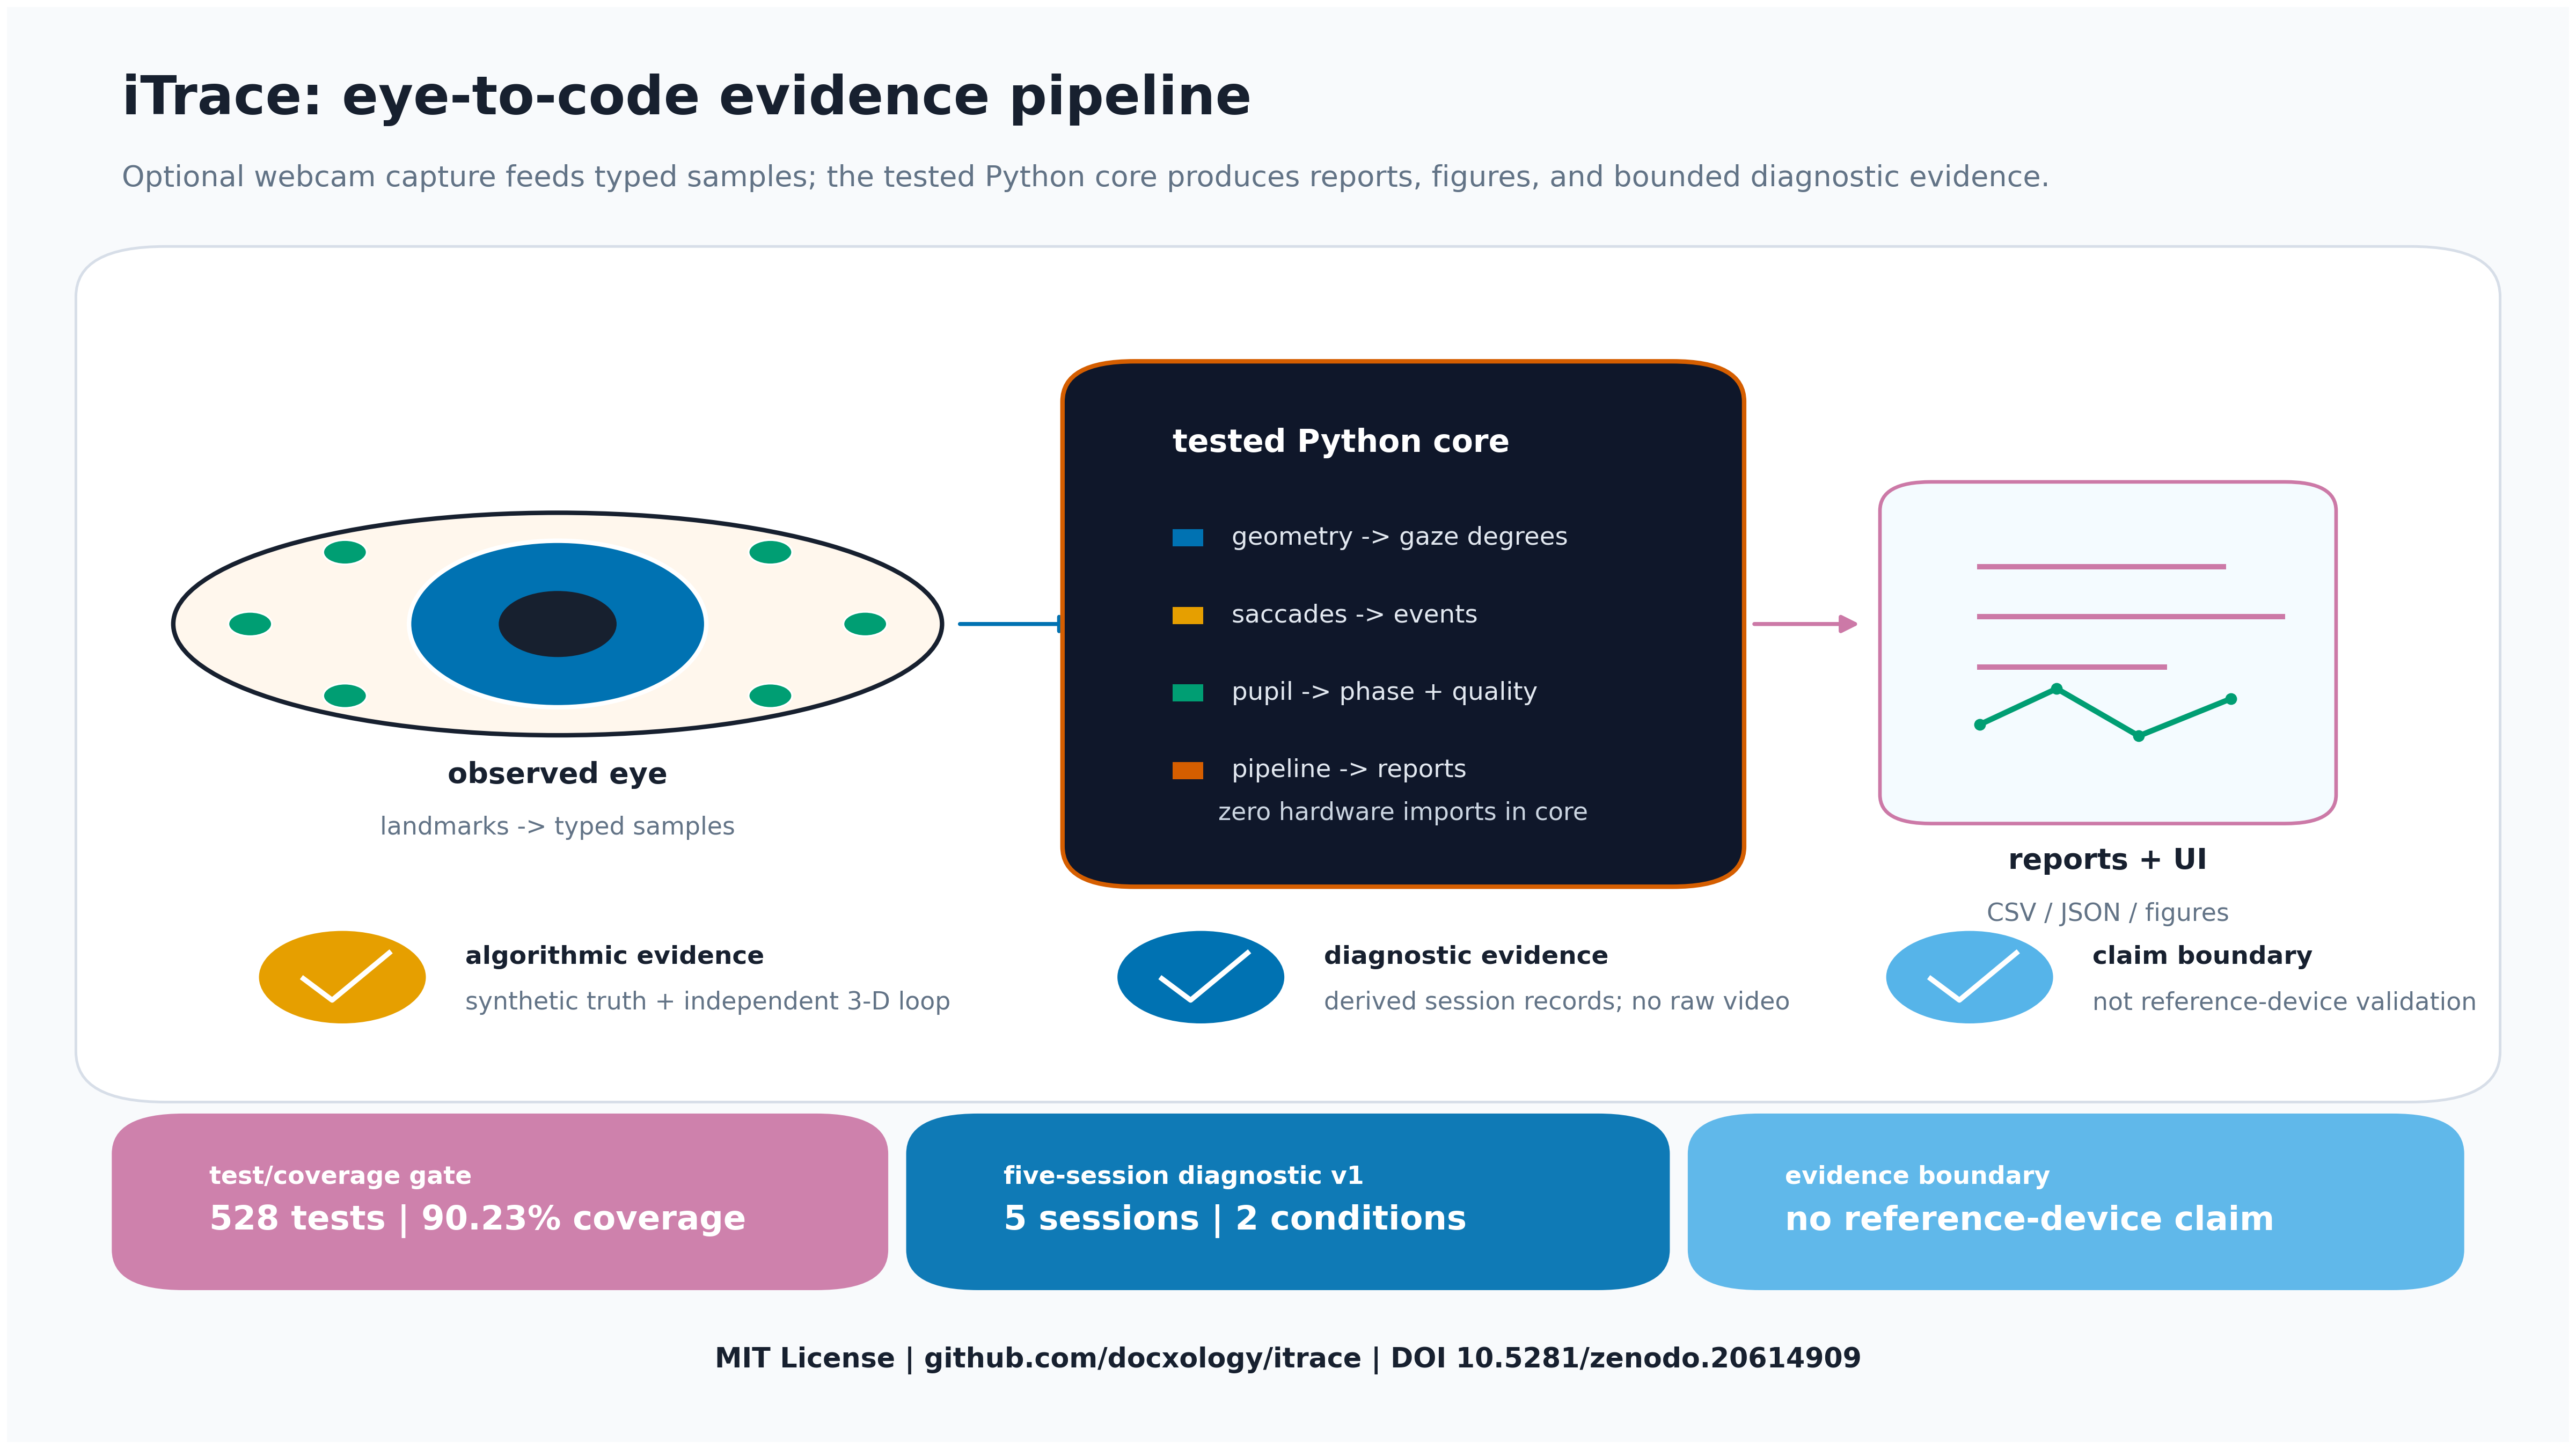
\includegraphics[width=1\linewidth,height=\textheight,keepaspectratio,alt={Graphical abstract of the iTrace eye-to-code evidence pipeline. A stylized observed eye feeds typed gaze, saccade, pupil, and quality records into the pure Python core, which then produces reports, figures, and live displays from Python-computed payloads. Three badges summarise the current verification gate, the five-session diagnostic v1 release scope, and the no-reference-device-claim boundary. The footer states MIT License, github.com/docxology/itrace, and the Zenodo DOI 10.5281/zenodo.20614027; the figure describes architecture and evidence boundaries, not webcam accuracy validation.}]{../output/figures/graphical_abstract.png}
\caption{Graphical abstract of the iTrace eye-to-code evidence pipeline.
A stylized observed eye feeds typed gaze, saccade, pupil, and quality
records into the pure Python core, which then produces reports, figures,
and live displays from Python-computed payloads. Three badges summarise
the current verification gate, the five-session diagnostic v1 release
scope, and the no-reference-device-claim boundary. The footer states MIT
License, github.com/docxology/itrace, and the Zenodo DOI
10.5281/zenodo.20614027; the figure describes architecture and evidence
boundaries, not webcam accuracy
validation.}\label{fig:graphical-abstract}
\end{figure}

\section{Results: ground-truth recovery}\label{sec:results}

The first question for any detector is whether it recovers events it
could not have peeked at. Every trace in this section is synthetic: a
generator builds the signal \emph{and} returns the parameters used to
build it, so the recovered numbers are checked against truth held out by
construction. None of these results speak to real-eye accuracy, which
remains the device validation gap of sec.~\ref{sec:limitations}. They
do, however, expose the kinds of implementation errors that matter
before hardware is involved: time-unit mistakes, coordinate sign flips,
threshold off-by-one boundaries, and accidental smoothing choices that
move event onsets.

On a synthetic fixation→saccade→fixation trace at 250 Hz, the I-VT
detector (\citeproc{ref-salvucci2000identifying}{Salvucci and Goldberg
2000}) recovers exactly one saccade bracketed by two fixations; the
recovered amplitude matches the constructed 10° to within 5\% and peak
velocity to within 10\% across the test grid. The min-jerk generator
sweeps amplitude and direction, and the recovered direction tracks the
constructed angle around the full circle (the gaze convention of 0°
right, +90° up), so a sign flip or axis swap on either path would
surface immediately. A purely-noisy fixation trace yields zero saccades
at the default threshold --- the anti-criterion confirming the detector
does not hallucinate events from noise.

The Engbert--Kliegl detector
(\citeproc{ref-engbert2003microsaccades}{Engbert and Kliegl 2003})
recovers an embedded 0.5° microsaccade from fixational jitter while
ignoring the surrounding noise; a probe confirms the threshold uses the
median-based robust estimator (it returns a value below half the plain
standard deviation in the presence of velocity outliers), the property
checked directly in sec.~\ref{sec:events}. Recovered microsaccade
amplitude and peak velocity fall on a tight, low-amplitude main-sequence
cluster, distinct from the large-saccade branch --- the expected
separation of the two scales rather than a fitted claim. The
main-sequence fit recovers the saturating \(V_{\max}\) and \(C\) of a
synthetic relationship (\citeproc{ref-bahill1975main}{Bahill et al.
1975}) to within 10\% and returns a power-law exponent inside the
physiological 0.4--0.9 range (fig.~\ref{fig:mainseq}).

\begin{figure}
\centering
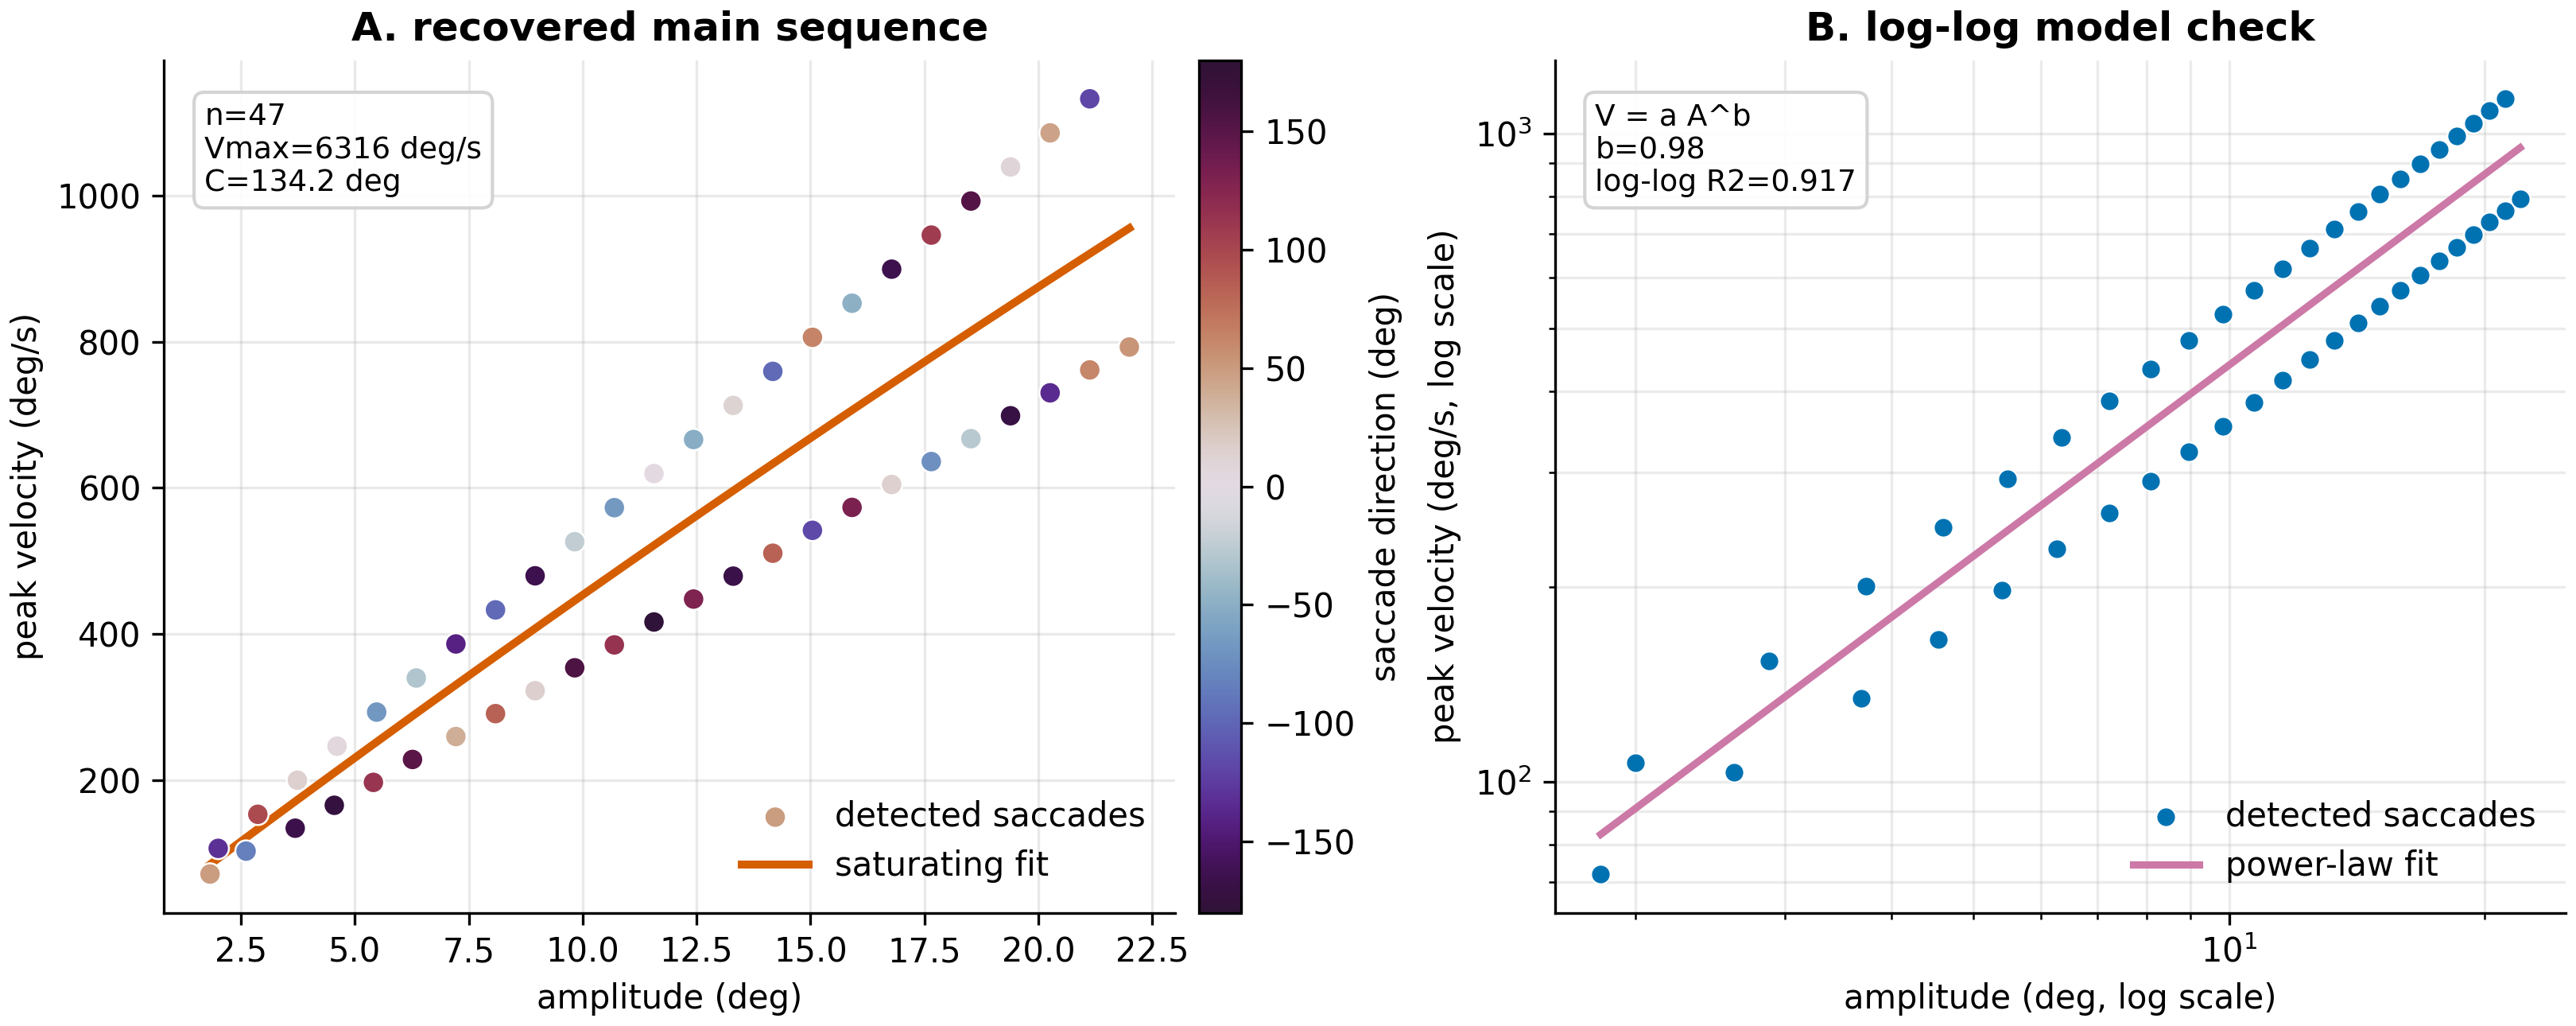
\includegraphics[width=1\linewidth,height=\textheight,keepaspectratio,alt={Main-sequence recovery from a synthetic multi-amplitude recording. Panel A plots detected saccades by amplitude, peak velocity, and direction, with the fitted saturating curve and recovered parameters. Panel B repeats the same detections on log-log axes with the fitted power law, making the exponent and goodness-of-fit explicit. The evidence is recovery of a seeded synthetic relationship and detector property extraction; it is not a physiological population estimate or real-device validation.}]{../output/figures/main_sequence.png}
\caption{Main-sequence recovery from a synthetic multi-amplitude
recording. Panel A plots detected saccades by amplitude, peak velocity,
and direction, with the fitted saturating curve and recovered
parameters. Panel B repeats the same detections on log-log axes with the
fitted power law, making the exponent and goodness-of-fit explicit. The
evidence is recovery of a seeded synthetic relationship and detector
property extraction; it is not a physiological population estimate or
real-device validation.}\label{fig:mainseq}
\end{figure}

\section{Results: pupillometry}\label{sec:pupilresults}

A sinusoidal pupil signal with an injected NaN blink is correctly
deblinked (no residual NaNs), and the interpolated-plus-smoothed trace
coincides with the underlying sine away from the blink window --- the
blink is bridged, not fabricated. A fully-invalid trace is reported as
unusable rather than silently flattened, so a recording the camera never
resolved cannot masquerade as a flat pupil. These are recovery checks
against a known generator, not statements about pupil-size accuracy on a
real eye (sec.~\ref{sec:limitations}). That distinction matters because
the pure pupil pipeline can verify blink handling, interpolation, phase
causality, and unit propagation even when the live webcam pupil proxy
remains a relative image-derived signal.

The causal phase detector labels peaks within a two-sample window of the
analytic sine maxima, and the online-equals-offline-prefix test confirms
it consults no future sample: replaying the signal one sample at a time
reproduces the offline labels exactly up to each prefix, so the
causality property of sec.~\ref{sec:pupillometry} holds empirically
rather than by assertion. The detected peak and trough counts match the
number of sine cycles in the trace, the coarsest sanity bound on the
detector. Saccade direction distributions over the same synthetic
sessions are summarised as polar histograms (fig.~\ref{fig:polar}).

\begin{figure}
\centering
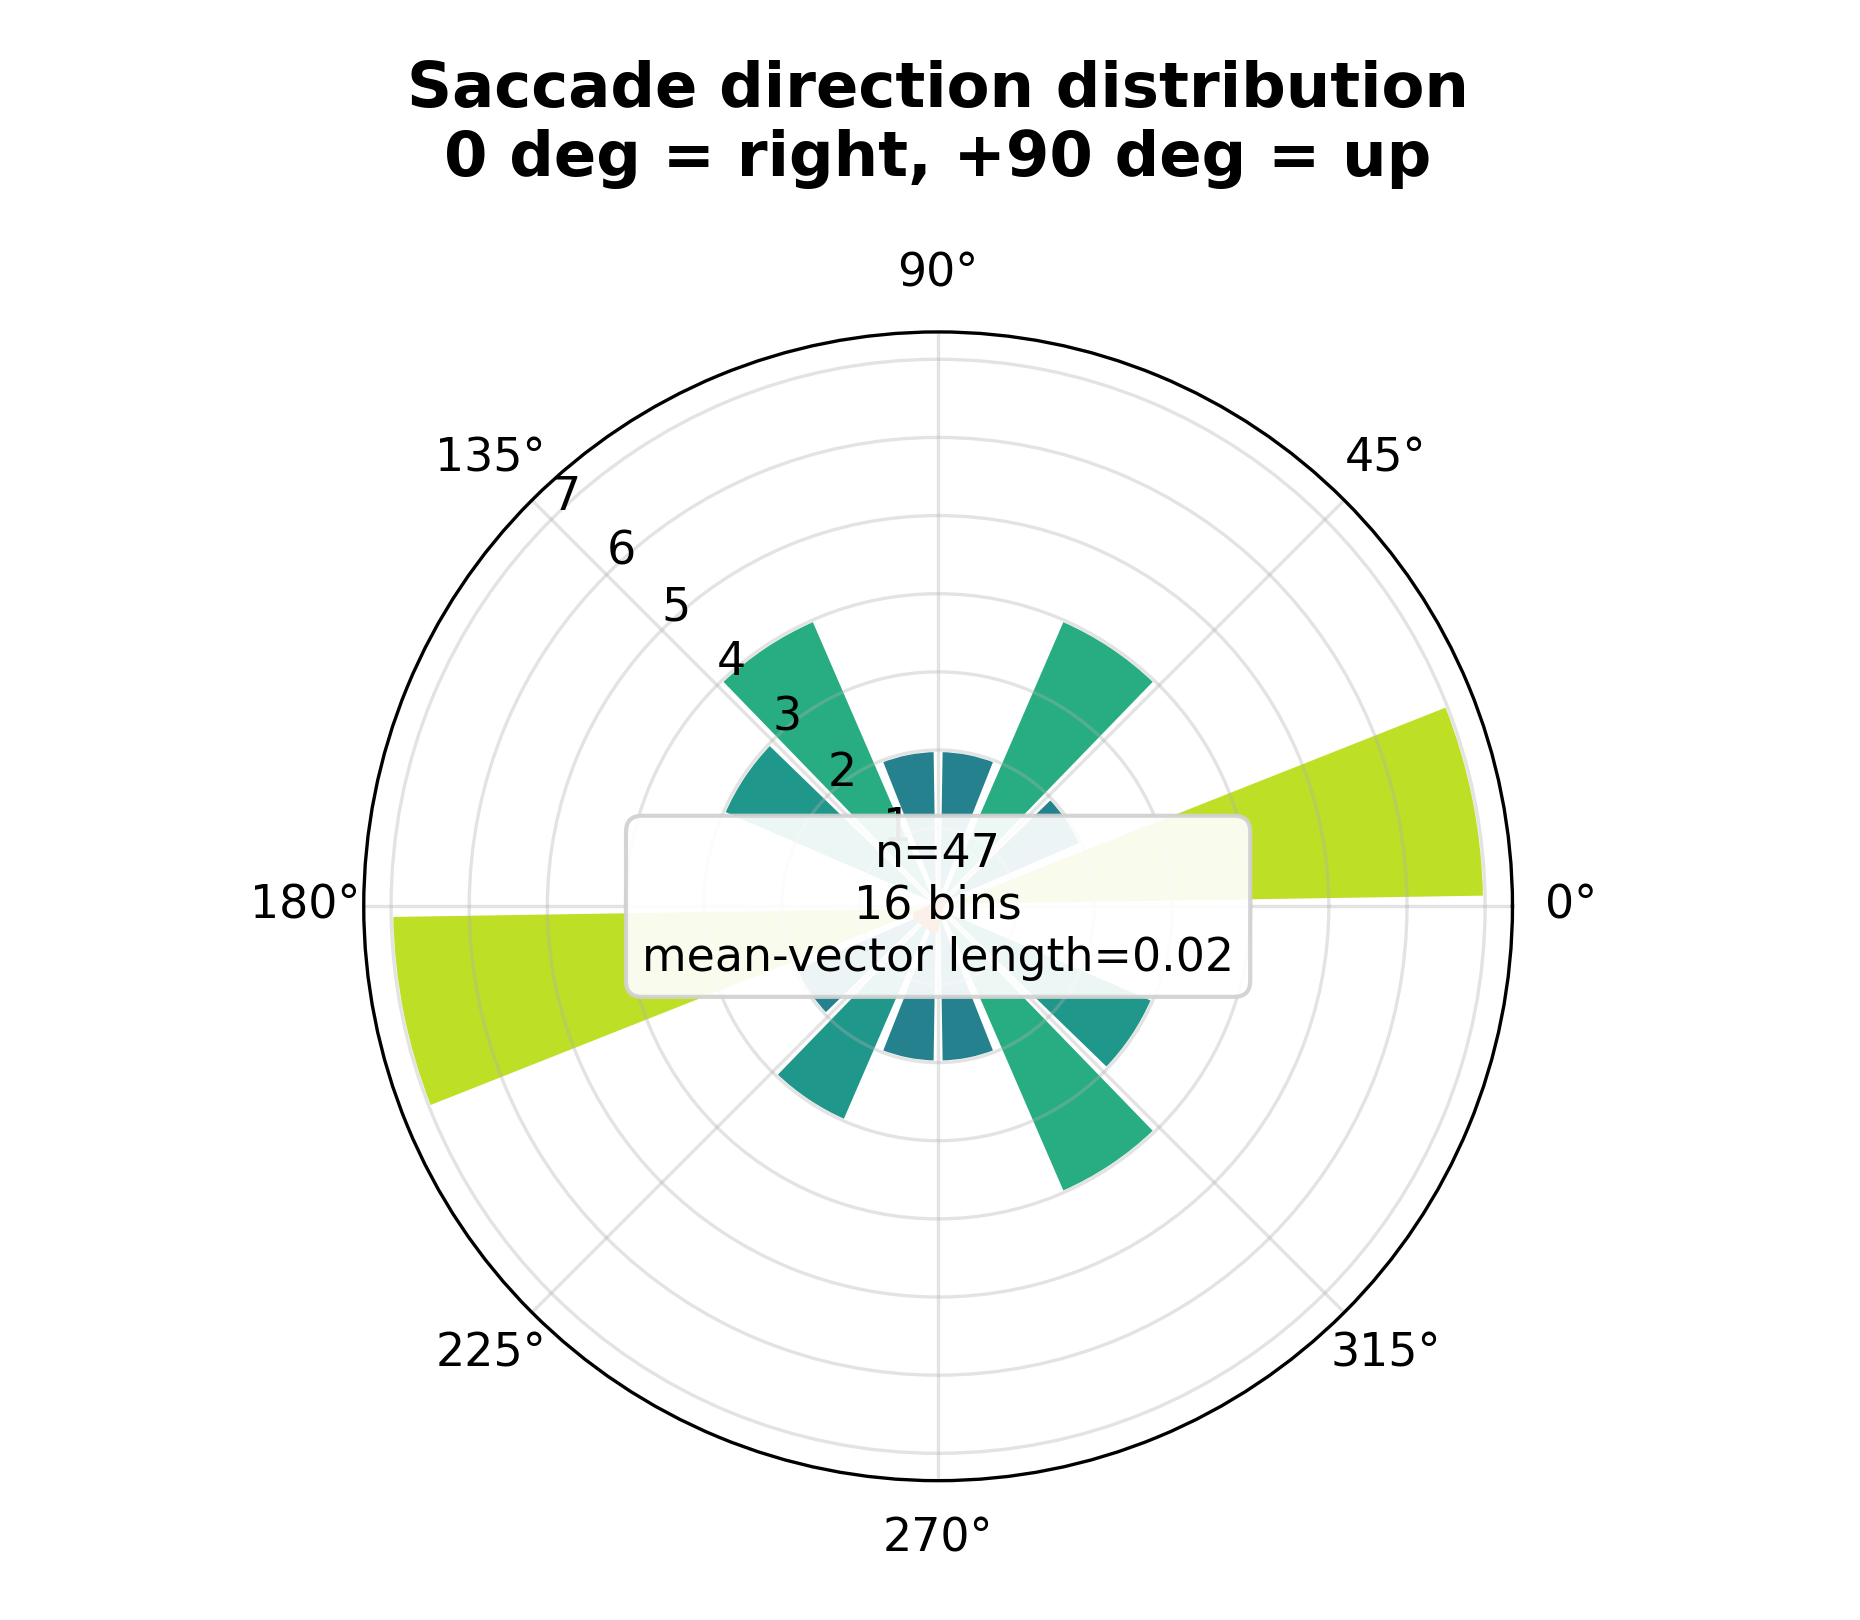
\includegraphics[width=0.75\linewidth,height=\textheight,keepaspectratio,alt={Saccade direction distribution over the synthetic multi-saccade recording. The polar convention is printed in the figure (0° = right, +90° = up), bars encode counts over 16 angular bins, and the orange resultant vector summarises directional balance. The panel verifies the package-wide direction convention and recovered event directions on synthetic data; it does not infer natural viewing bias.}]{../output/figures/direction_polar.png}
\caption{Saccade direction distribution over the synthetic multi-saccade
recording. The polar convention is printed in the figure (0° = right,
+90° = up), bars encode counts over 16 angular bins, and the orange
resultant vector summarises directional balance. The panel verifies the
package-wide direction convention and recovered event directions on
synthetic data; it does not infer natural viewing
bias.}\label{fig:polar}
\end{figure}

\section{Results: closed-loop recovery}\label{sec:closedloop}

Running the full loop --- 3-D eyeball → perspective projection →
landmark extraction → estimation → recovery --- on the default animated
scene (four fixations joined by three saccades, two pupil dilation
events, one blink, at 120 Hz) recovers gaze with an RMS residual of
\textbf{0.16°} against the 3-D truth (maximum 0.23°) for gaze within
±15°, and recovers the three scripted saccades exactly
(fig.~\ref{fig:loop}). The residual is small but strictly non-zero,
confirming the forward model and estimator are independent
(sec.~\ref{sec:forward}).

This is an \emph{internal-consistency verification}: it proves the
estimator correctly inverts the forward model and would expose sign
flips, axis swaps, unit errors, and coordinate-frame mismatches. It is
\textbf{not} device validation. The 0.16° is a \emph{lower bound} on
real-world error --- any idealization the two paths share (pinhole
projection, no corneal refraction, a spherical eye, zero kappa)
contributes exactly zero residual by construction
(sec.~\ref{sec:limitations}). The recovered pupil (\(r = 1.0\)) is a
near-identity consistency check (the projected pupil/iris ratio is a
monotone function of pupil radius), confirming the deblink/pipeline
preserve the signal --- not pupil-size accuracy. This is the strongest
possible evidence for software geometry consistency inside the current
assumptions and deliberately weaker evidence for the real optical
system.

\begin{figure}
\centering
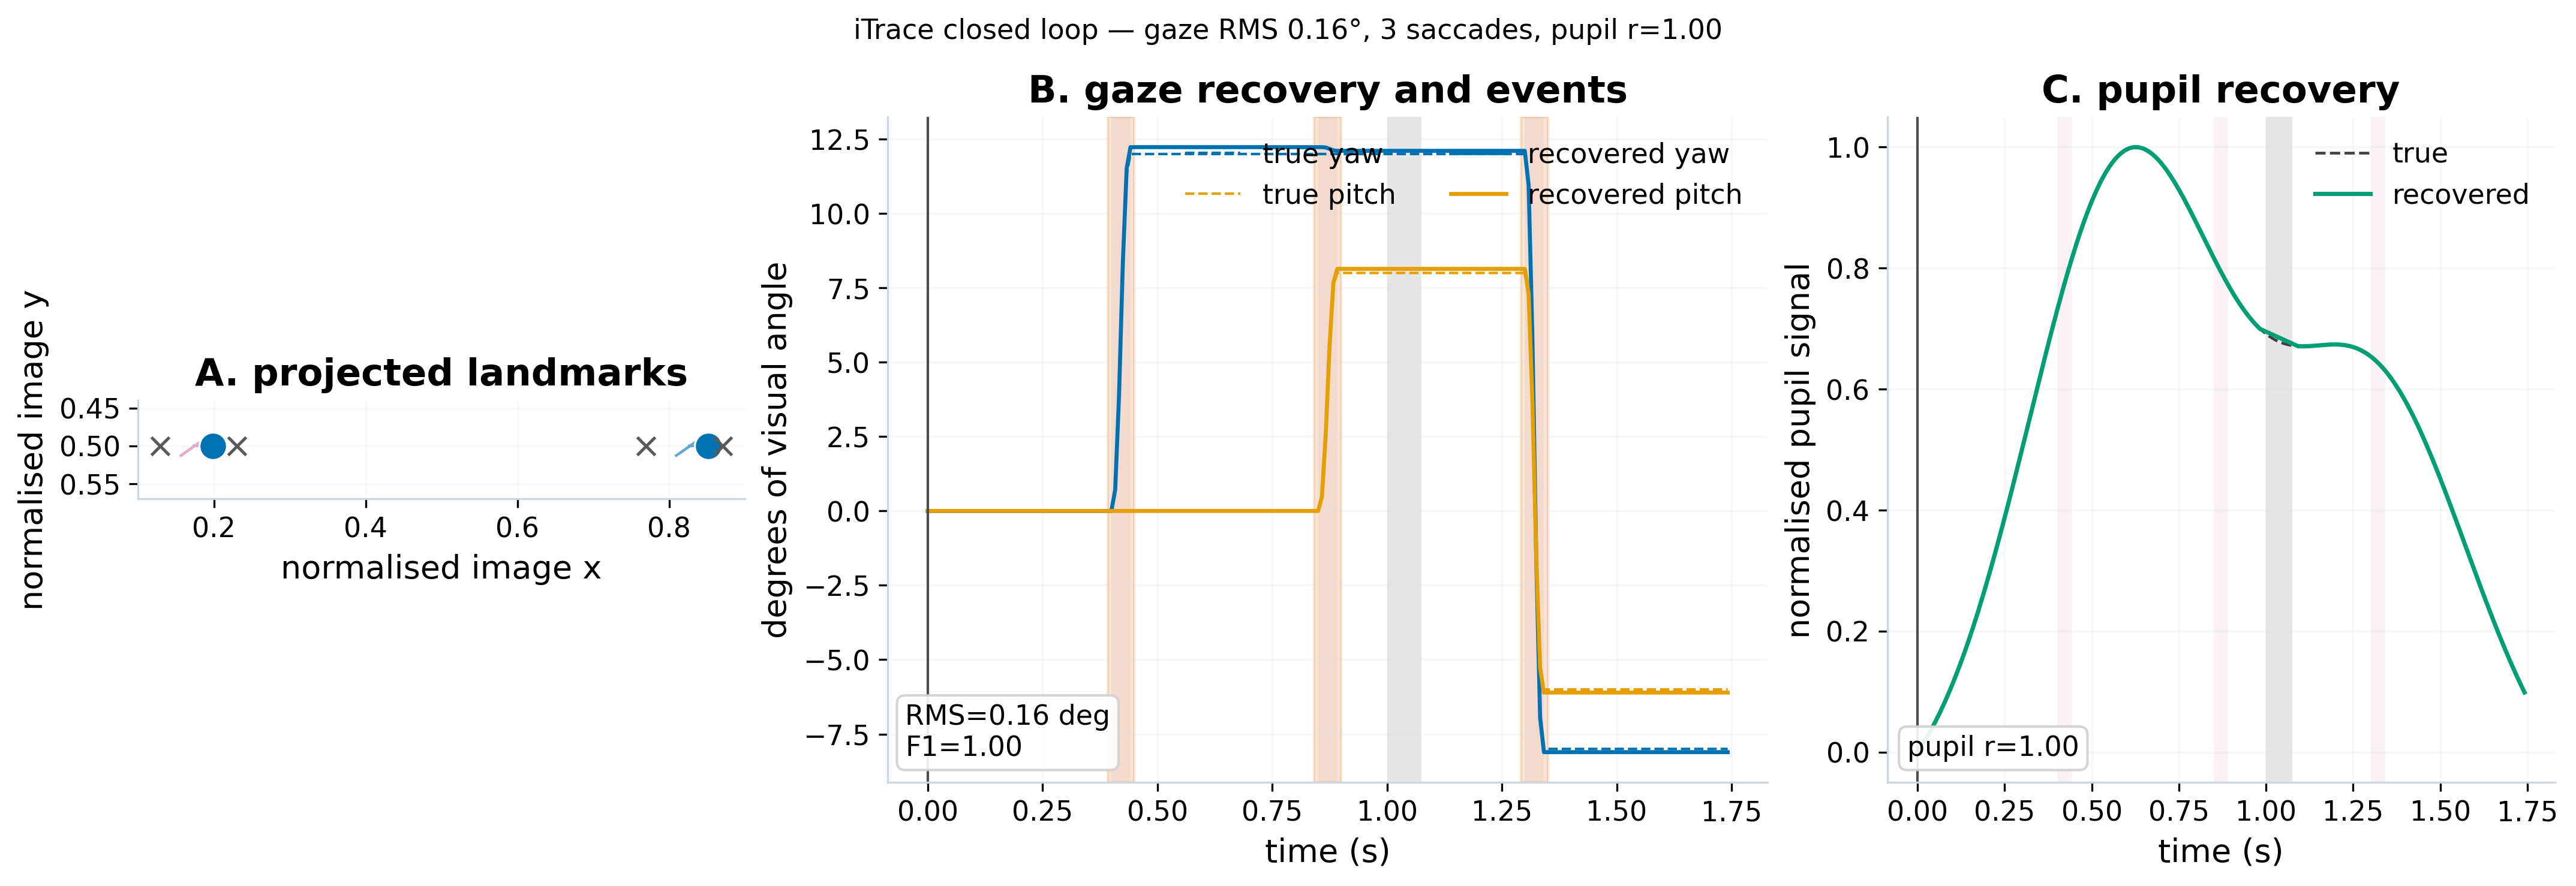
\includegraphics[width=1\linewidth,height=\textheight,keepaspectratio,alt={Closed-loop recovery on the default synthetic scene. Panel A shows the projected binocular landmark geometry and the two iris-centre paths. Panel B overlays true and recovered yaw/pitch, with scripted and detected saccade intervals shaded. Panel C overlays true and recovered pupil dynamics after normalisation, with the blink interval shaded. The figure verifies consistency between an independent 3-D generator and the estimator; shared idealisations mean the residual is a lower bound, not a measured webcam error.}]{../output/figures/closed_loop_summary.png}
\caption{Closed-loop recovery on the default synthetic scene. Panel A
shows the projected binocular landmark geometry and the two iris-centre
paths. Panel B overlays true and recovered yaw/pitch, with scripted and
detected saccade intervals shaded. Panel C overlays true and recovered
pupil dynamics after normalisation, with the blink interval shaded. The
figure verifies consistency between an independent 3-D generator and the
estimator; shared idealisations mean the residual is a lower bound, not
a measured webcam error.}\label{fig:loop}
\end{figure}

The synthetic generator supplies all three target signals jointly ---
gaze direction, saccade intervals, and pupil diameter --- animated as
floating 3-D eyeball orbs (fig.~\ref{fig:orbs}).

\begin{figure}
\centering
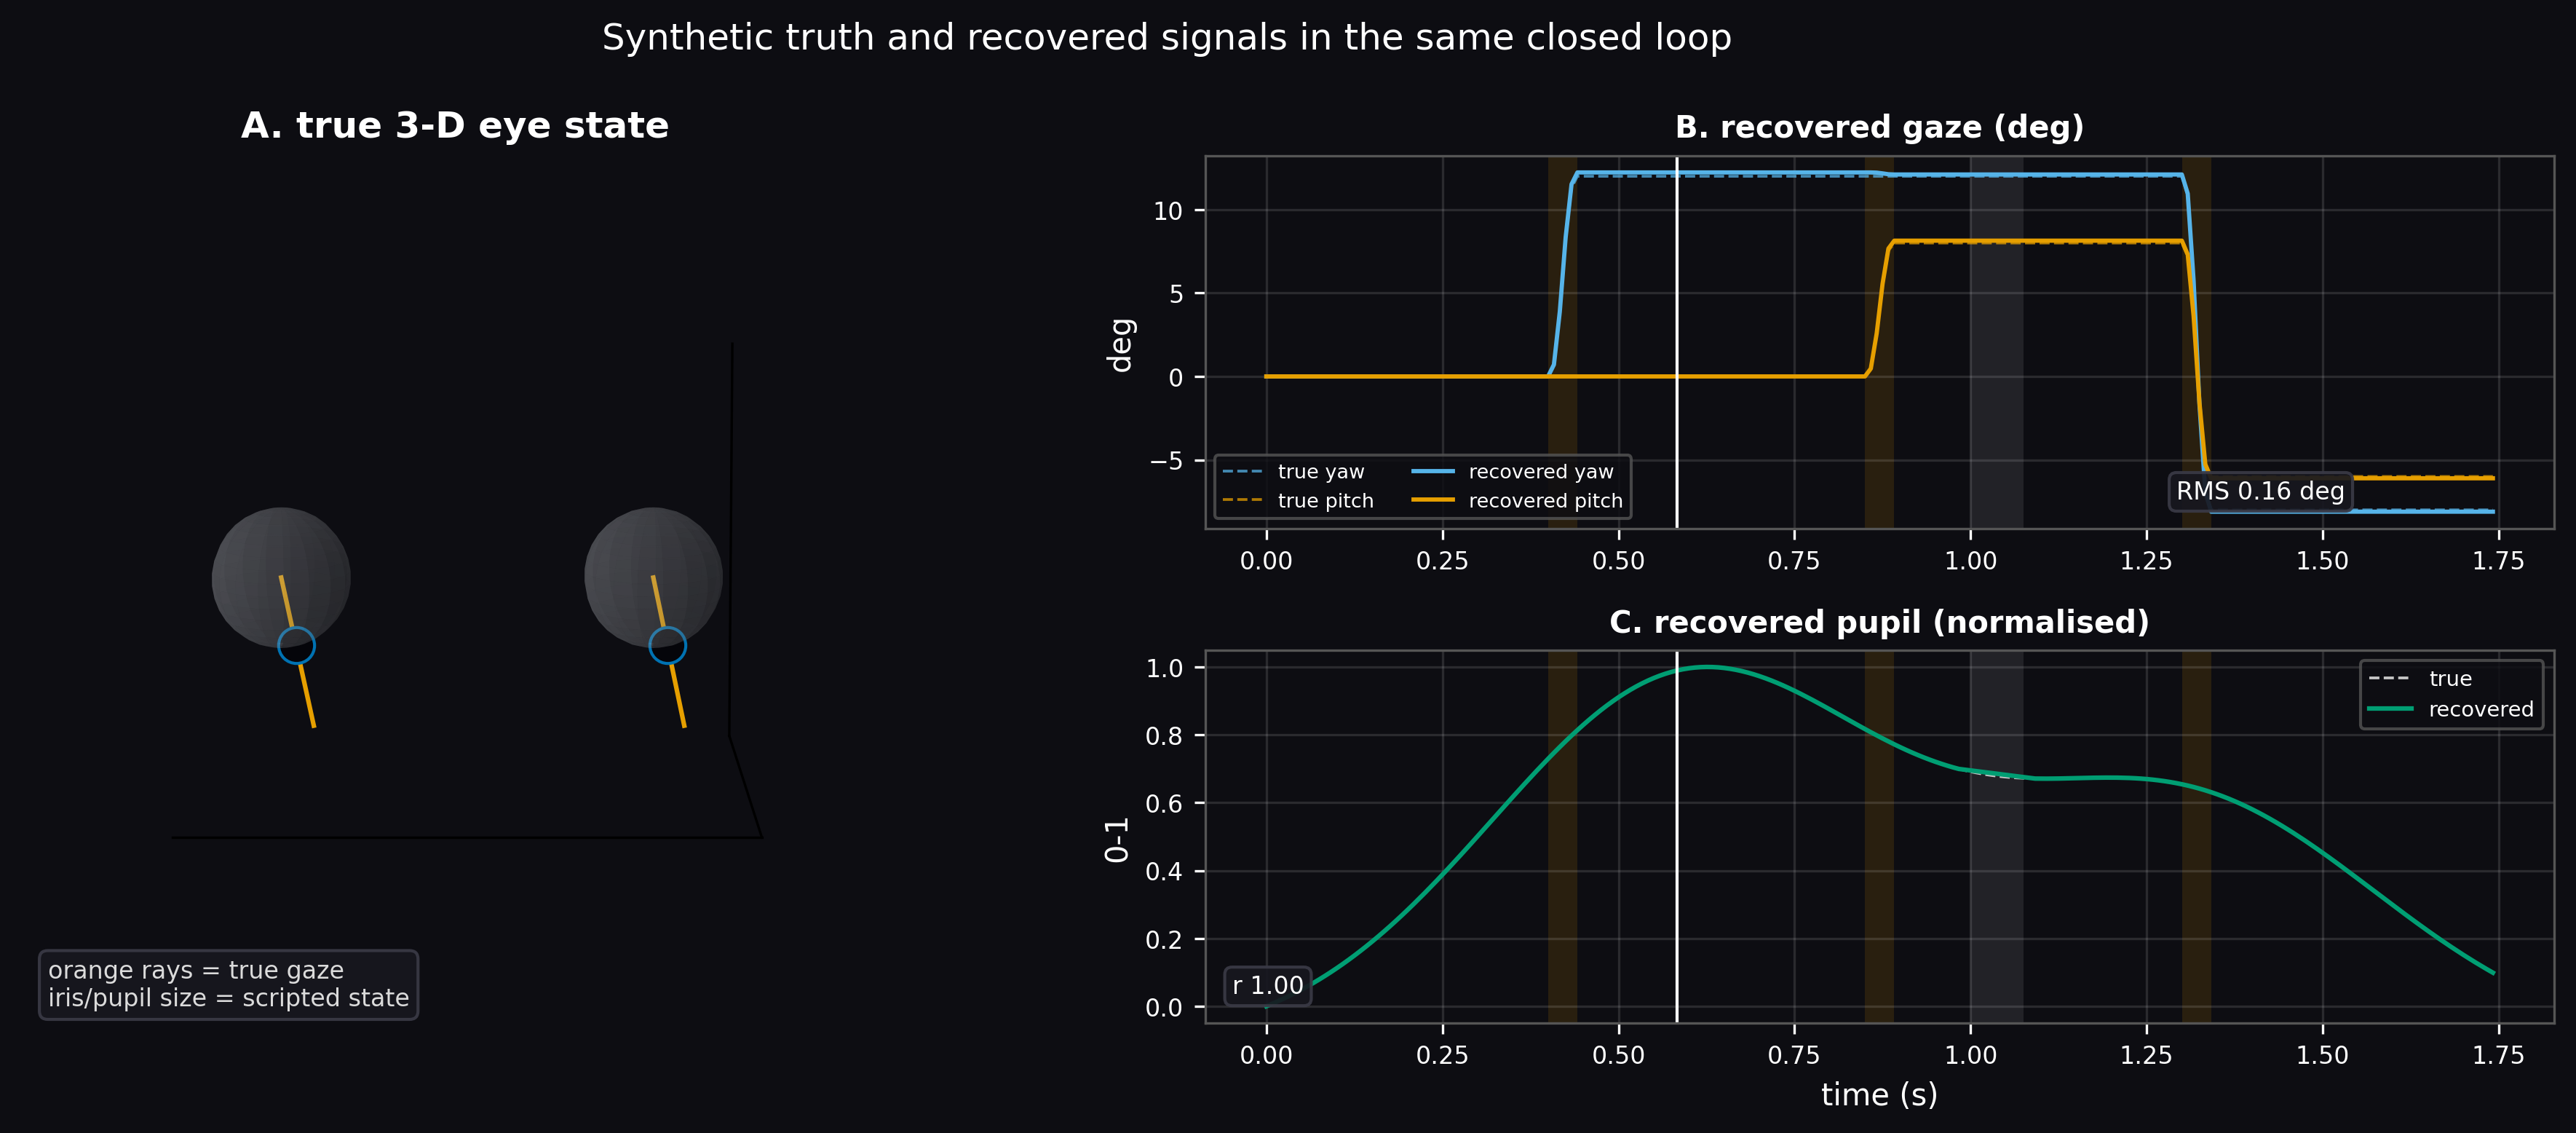
\includegraphics[width=1\linewidth,height=\textheight,keepaspectratio,alt={Synthetic truth and recovered signals rendered together. The 3-D panel shows the true eyeball orientation, gaze rays, iris, and pupil state at one representative frame; the trace panels repeat the recovered yaw, pitch, and pupil signals with true values, saccades, and the blink interval visible for audit. This panel is a visual audit of the synthetic scene and recovery path, not evidence from a recorded participant.}]{../output/figures/eye_orbs_still.png}
\caption{Synthetic truth and recovered signals rendered together. The
3-D panel shows the true eyeball orientation, gaze rays, iris, and pupil
state at one representative frame; the trace panels repeat the recovered
yaw, pitch, and pupil signals with true values, saccades, and the blink
interval visible for audit. This panel is a visual audit of the
synthetic scene and recovery path, not evidence from a recorded
participant.}\label{fig:orbs}
\end{figure}

\section{Results: noise-sensitivity analysis}\label{sec:noiseresults}

Sweeping the landmark-noise standard deviation \(\sigma\) from 0 to
0.016 (normalised image units), 25 seeded trials per level, gives a
clear and differentiated degradation of the three signals
(fig.~\ref{fig:power}, tbl.~\ref{tbl:noise}). The sweep is intentionally
idealised: it injects independent landmark noise into the same synthetic
scene rather than replaying real MediaPipe failures, so its value is to
rank algorithmic fragilities under controlled perturbation.

\textbf{Gaze} RMS error rises monotonically and approximately linearly
with \(\sigma\), crossing the 2° usability bound at
\(\sigma \approx 0.005\). \textbf{Saccade} detection is the most fragile
emergent signal: F1 falls below 0.8 already at \(\sigma \approx 0.0014\)
--- a direct consequence of detection resting on the velocity, the
time-derivative of position, which amplifies high-frequency noise. Both
orderings \emph{emerge} from propagating landmark noise through the real
estimator.

The \textbf{pupil} result carries a sharp caveat: its robustness
(correlation above 0.9 until \(\sigma \approx 0.005\)) is \textbf{robust
by construction} under the assumed \texttt{pupil\_noise\_scale}, not a
measured property, and would move if that parameter changed. It is
reported as a conditional illustration, not a finding; the genuine
emergent result is the gaze-vs-saccade ordering.

The most defensible practical takeaway comes from translating \(\sigma\)
to pixels. At a 640 px width, the saccade breakdown at
\(\sigma \approx 0.0014\) is \(\approx 0.9\) px, whereas gaze tolerates
roughly three pixels in this idealised sweep. That pixel-scale
comparison is not a universal detector specification: real webcam
landmark error is camera-, pose-, lighting-, compression-, and
algorithm-dependent. It does show why webcam saccade \emph{timing} is
theoretically marginal before any real-world bias, temporal correlation,
or tracking dropout is added, while coarse fixation and gaze direction
have more headroom.

The N=1 empirical target residual in sec.~\ref{sec:empirical-pilot} is
much larger than the residuals in this idealised landmark-noise sweep
for the expected reason: it bundles calibration, screen-prompt,
user-compliance, target-eccentricity, timestamp, and webcam-session
effects into one prompted-target diagnostic. That makes it useful for
bounding realistic live-demo and stress-test ranges, but it should not
be back-solved into an iid landmark-noise \(\sigma\) or treated as
reference-device gaze accuracy.

\begin{figure}
\centering
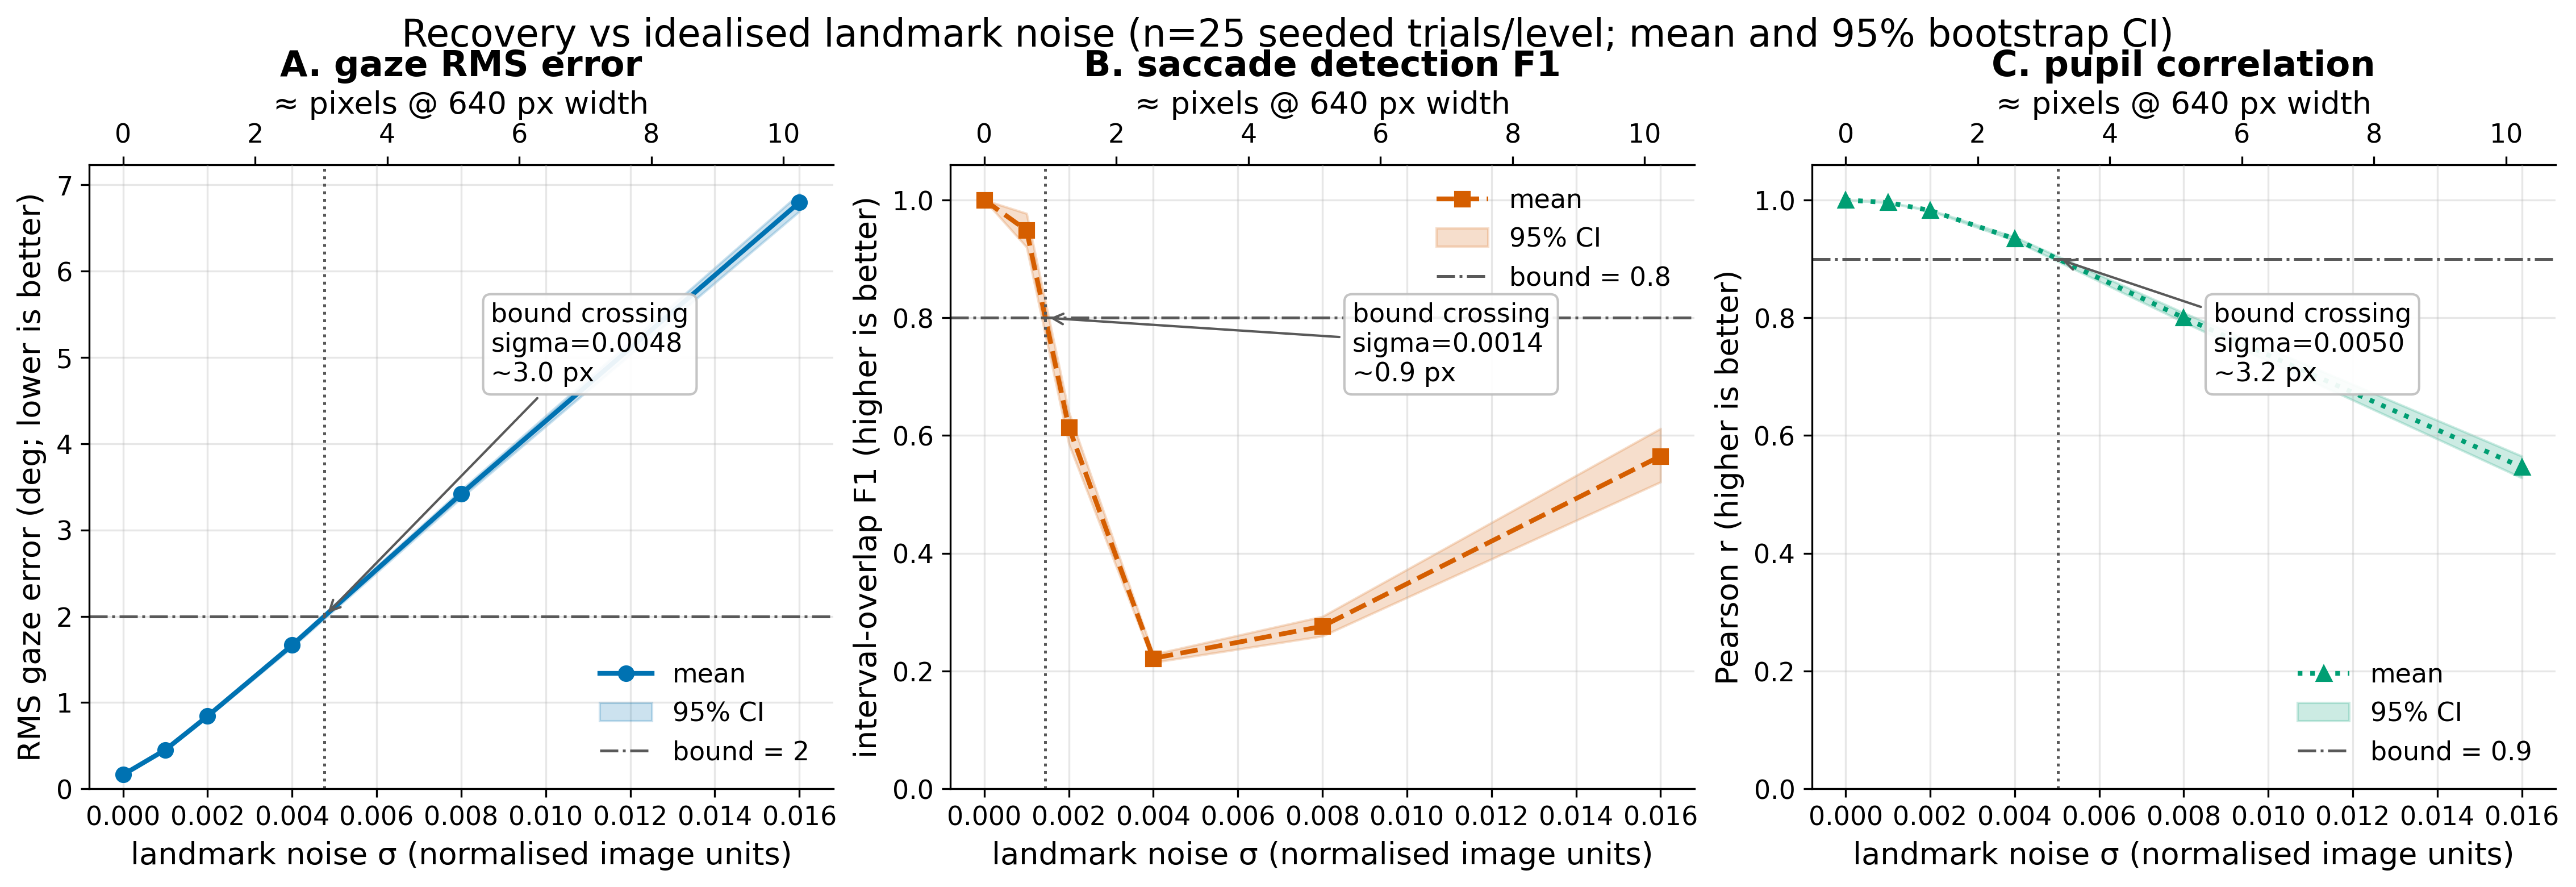
\includegraphics[width=1\linewidth,height=\textheight,keepaspectratio,alt={Recovery vs idealised webcam observation noise. Each panel reports the Monte-Carlo mean and 95\% bootstrap confidence band for one recovered signal, with the manuscript usability bound drawn as a horizontal line and the interpolated bound crossing annotated in both normalised σ and approximate pixels at 640 px width. Colour, marker, and line style all encode the signal so the figure remains legible in greyscale. The figure supports an algorithmic fragility ordering under iid landmark perturbations; it does not measure MediaPipe, lens, illumination, head-pose, or calibration error on real frames.}]{../output/figures/noise_power.png}
\caption{Recovery vs idealised webcam observation noise. Each panel
reports the Monte-Carlo mean and 95\% bootstrap confidence band for one
recovered signal, with the manuscript usability bound drawn as a
horizontal line and the interpolated bound crossing annotated in both
normalised σ and approximate pixels at 640 px width. Colour, marker, and
line style all encode the signal so the figure remains legible in
greyscale. The figure supports an algorithmic fragility ordering under
iid landmark perturbations; it does not measure MediaPipe, lens,
illumination, head-pose, or calibration error on real
frames.}\label{fig:power}
\end{figure}

The same numbers, with per-cell uncertainty, are the generated
statistics table (tbl.~\ref{tbl:noise}); it and the figure are generated
from one sweep so they never drift. (Snapshot at \(n=25\); regenerate
with \texttt{scripts/generate\_power\_figure.py}.)

\begin{longtable}[]{@{}
  >{\raggedright\arraybackslash}p{(\linewidth - 8\tabcolsep) * \real{0.2000}}
  >{\raggedright\arraybackslash}p{(\linewidth - 8\tabcolsep) * \real{0.2000}}
  >{\raggedright\arraybackslash}p{(\linewidth - 8\tabcolsep) * \real{0.2000}}
  >{\raggedright\arraybackslash}p{(\linewidth - 8\tabcolsep) * \real{0.2000}}
  >{\raggedright\arraybackslash}p{(\linewidth - 8\tabcolsep) * \real{0.2000}}@{}}
\caption{Recovery vs landmark noise σ (mean ± 95\% half-CI,
\(n=25\)).}\label{tbl:noise}\tabularnewline
\toprule\noalign{}
\begin{minipage}[b]{\linewidth}\raggedright
sigma (norm)
\end{minipage} & \begin{minipage}[b]{\linewidth}\raggedright
sigma (px@640)
\end{minipage} & \begin{minipage}[b]{\linewidth}\raggedright
gaze RMS (deg)
\end{minipage} & \begin{minipage}[b]{\linewidth}\raggedright
saccade F1
\end{minipage} & \begin{minipage}[b]{\linewidth}\raggedright
pupil r
\end{minipage} \\
\midrule\noalign{}
\endfirsthead
\toprule\noalign{}
\begin{minipage}[b]{\linewidth}\raggedright
sigma (norm)
\end{minipage} & \begin{minipage}[b]{\linewidth}\raggedright
sigma (px@640)
\end{minipage} & \begin{minipage}[b]{\linewidth}\raggedright
gaze RMS (deg)
\end{minipage} & \begin{minipage}[b]{\linewidth}\raggedright
saccade F1
\end{minipage} & \begin{minipage}[b]{\linewidth}\raggedright
pupil r
\end{minipage} \\
\midrule\noalign{}
\endhead
\bottomrule\noalign{}
\endlastfoot
0.0000 & 0.00 & 0.163 +/- 0.000 & 1.000 +/- 0.000 & 1.000 +/- 0.000 \\
0.0010 & 0.64 & 0.452 +/- 0.006 & 0.949 +/- 0.029 & 0.996 +/- 0.000 \\
0.0020 & 1.28 & 0.842 +/- 0.012 & 0.614 +/- 0.027 & 0.982 +/- 0.001 \\
0.0040 & 2.56 & 1.665 +/- 0.026 & 0.222 +/- 0.007 & 0.934 +/- 0.003 \\
0.0080 & 5.12 & 3.418 +/- 0.046 & 0.276 +/- 0.017 & 0.800 +/- 0.008 \\
0.0160 & 10.24 & 6.798 +/- 0.102 & 0.565 +/- 0.045 & 0.546 +/- 0.018 \\
\end{longtable}

\section{Results: cross-implementation agreement and
gates}\label{sec:reproducibility}

On a shared synthetic trace the core I-VT and microsaccade detectors
agree with an independent reference implementation
(\texttt{reference\_impl}, raw finite-difference velocity and an
explicit-loop microsaccade detector) on event count and onset timing,
despite using different velocity formulations --- a guard against a bug
shared by a single implementation. The two paths share only their input
and the published algorithm definitions, so agreement is evidence the
implementation matches the algorithm, not that two copies of one mistake
agree.

The complete toolchain is green and reproducible: 528 no-mocks tests
pass with 90.23\% statement-and-branch coverage, \texttt{ruff} and
\texttt{ruff\ format} report no issues, and \texttt{mypy\ -\/-strict}
finds no type errors across the source tree. The test count, coverage,
version, gate date, and render evidence are stored once in
\texttt{docs/verification\_metrics.json}; the manuscript renderer
hydrates these tokens from that JSON so stale literal metrics are caught
by tests rather than silently carried into public artifacts. Every
synthetic generator and every Monte-Carlo trial is explicitly seeded
with \texttt{numpy.random.default\_rng}, so each figure and table number
is reproducible byte-for-byte from a clean checkout --- re-running the
figure pipeline twice produces identical PNGs, and the noise sweep of
sec.~\ref{sec:noiseresults} reproduces its table cells exactly. No test
mocks a computation: detectors run on real arrays with known ground
truth, file I/O uses real temporary files, and figures are asserted to
write non-empty PNGs. The full module map, dependency contract, and test
strategy are in sec.~\ref{sec:software}.

The documentation and visualization layer now follows the same evidence
rule. \texttt{docs/TRACEABILITY\_MATRIX.json} maps each public
validation claim and manuscript figure to the documentation surface
where it appears, the tested Python method or script that computes it,
the backing test file, the generated evidence artifact, and the truth
boundary. That matrix is deliberately machine-readable: tests verify its
paths and pure-core symbols, so a future figure, README badge, or
live-analysis claim cannot become orphaned prose detached from the
tested methods underneath it.

The validation-domain suite extends that reproducibility contract from a
single trace to stress domains. \texttt{itrace\ synthetic-validation}
writes JSON for repeated clean, webcam-jitter, head-drift, and
low-light/dropout sessions, summarising within-domain recovery and
across-domain stability. The live HTML page calls the same Python route
when the user runs synthetic validation from the browser; the browser
only renders the returned statistics and does not reimplement event
detection or recovery scoring.

Finally, \texttt{itrace\ benchmark} provides a release-ready shape for
external validation without pretending such data are bundled. It loads
caller-supplied truth and comparator event CSV files, can score a gaze
CSV through the iTrace pipeline, and writes one JSON report with
interval-overlap recovery plus timing and amplitude errors for each
system. That design matters because it separates the \emph{mechanism}
for validation from the \emph{evidence} required to make a validation
claim: the package can compute the same metrics against a reference
tracker, public dataset, or comparator detector, but the report must
carry the supplied truth source and boundary. A high score against
another detector is detector agreement; a high score against an
independent reference device would be a different and stronger claim.

The live experiment report follows the same reproducibility pattern for
real webcam sessions. \texttt{itrace\ live-html} auto-saves a derived
experiment bundle after the final required guided trial, and
\texttt{itrace\ experiment-report} rebuilds the empirical summary from
the exported manifest plus capture-record CSV. That command path is
intentionally file-based: the reported jitter, drift, finite fraction,
calibration residual, and target latency can be regenerated without a
browser or camera, while the payload still states that prompted screen
targets are not a reference-device validation study. The
manuscript-facing single-pilot summary in fig.~\ref{fig:empirical-pilot}
is hydrated from that report when it exists; when it does not, the same
render path exposes pending or unavailable fields rather than replacing
missing empirical data with guessed values.

\section{Results: single-pilot empirical
diagnostics}\label{sec:empirical-pilot}

The live empirical workflow is included here as an \textbf{N=1,
order-of-magnitude case study}, not as a participant study or device
validation claim. One local webcam session records fixed-gaze, reading,
and center/four-corner target trials; the backend stores derived capture
records, a protocol manifest, a target schedule, and an experiment
report; and the manuscript renderer reads only the small summary JSON
produced from that report. The current pilot source reports \textbf{3
completed trials, 2690 derived samples}. From that derived bundle, the
renderer hydrates the session metrics as follows: finite-gaze fraction
\textbf{100.0\%}, sampling rate \textbf{29.7 Hz}, sampling-interval
coefficient of variation \textbf{0.161}, maximum drift \textbf{0.054
deg/s}, held-out target RMS \textbf{6.79 deg}, and target acquisition
latency \textbf{0.72 s median}. The values are stored in
\texttt{docs/empirical\_pilot\_metrics.json}; when the pilot export is
absent, the same render path leaves each field explicitly unavailable
rather than filling a guessed value.

\begin{figure}
\centering
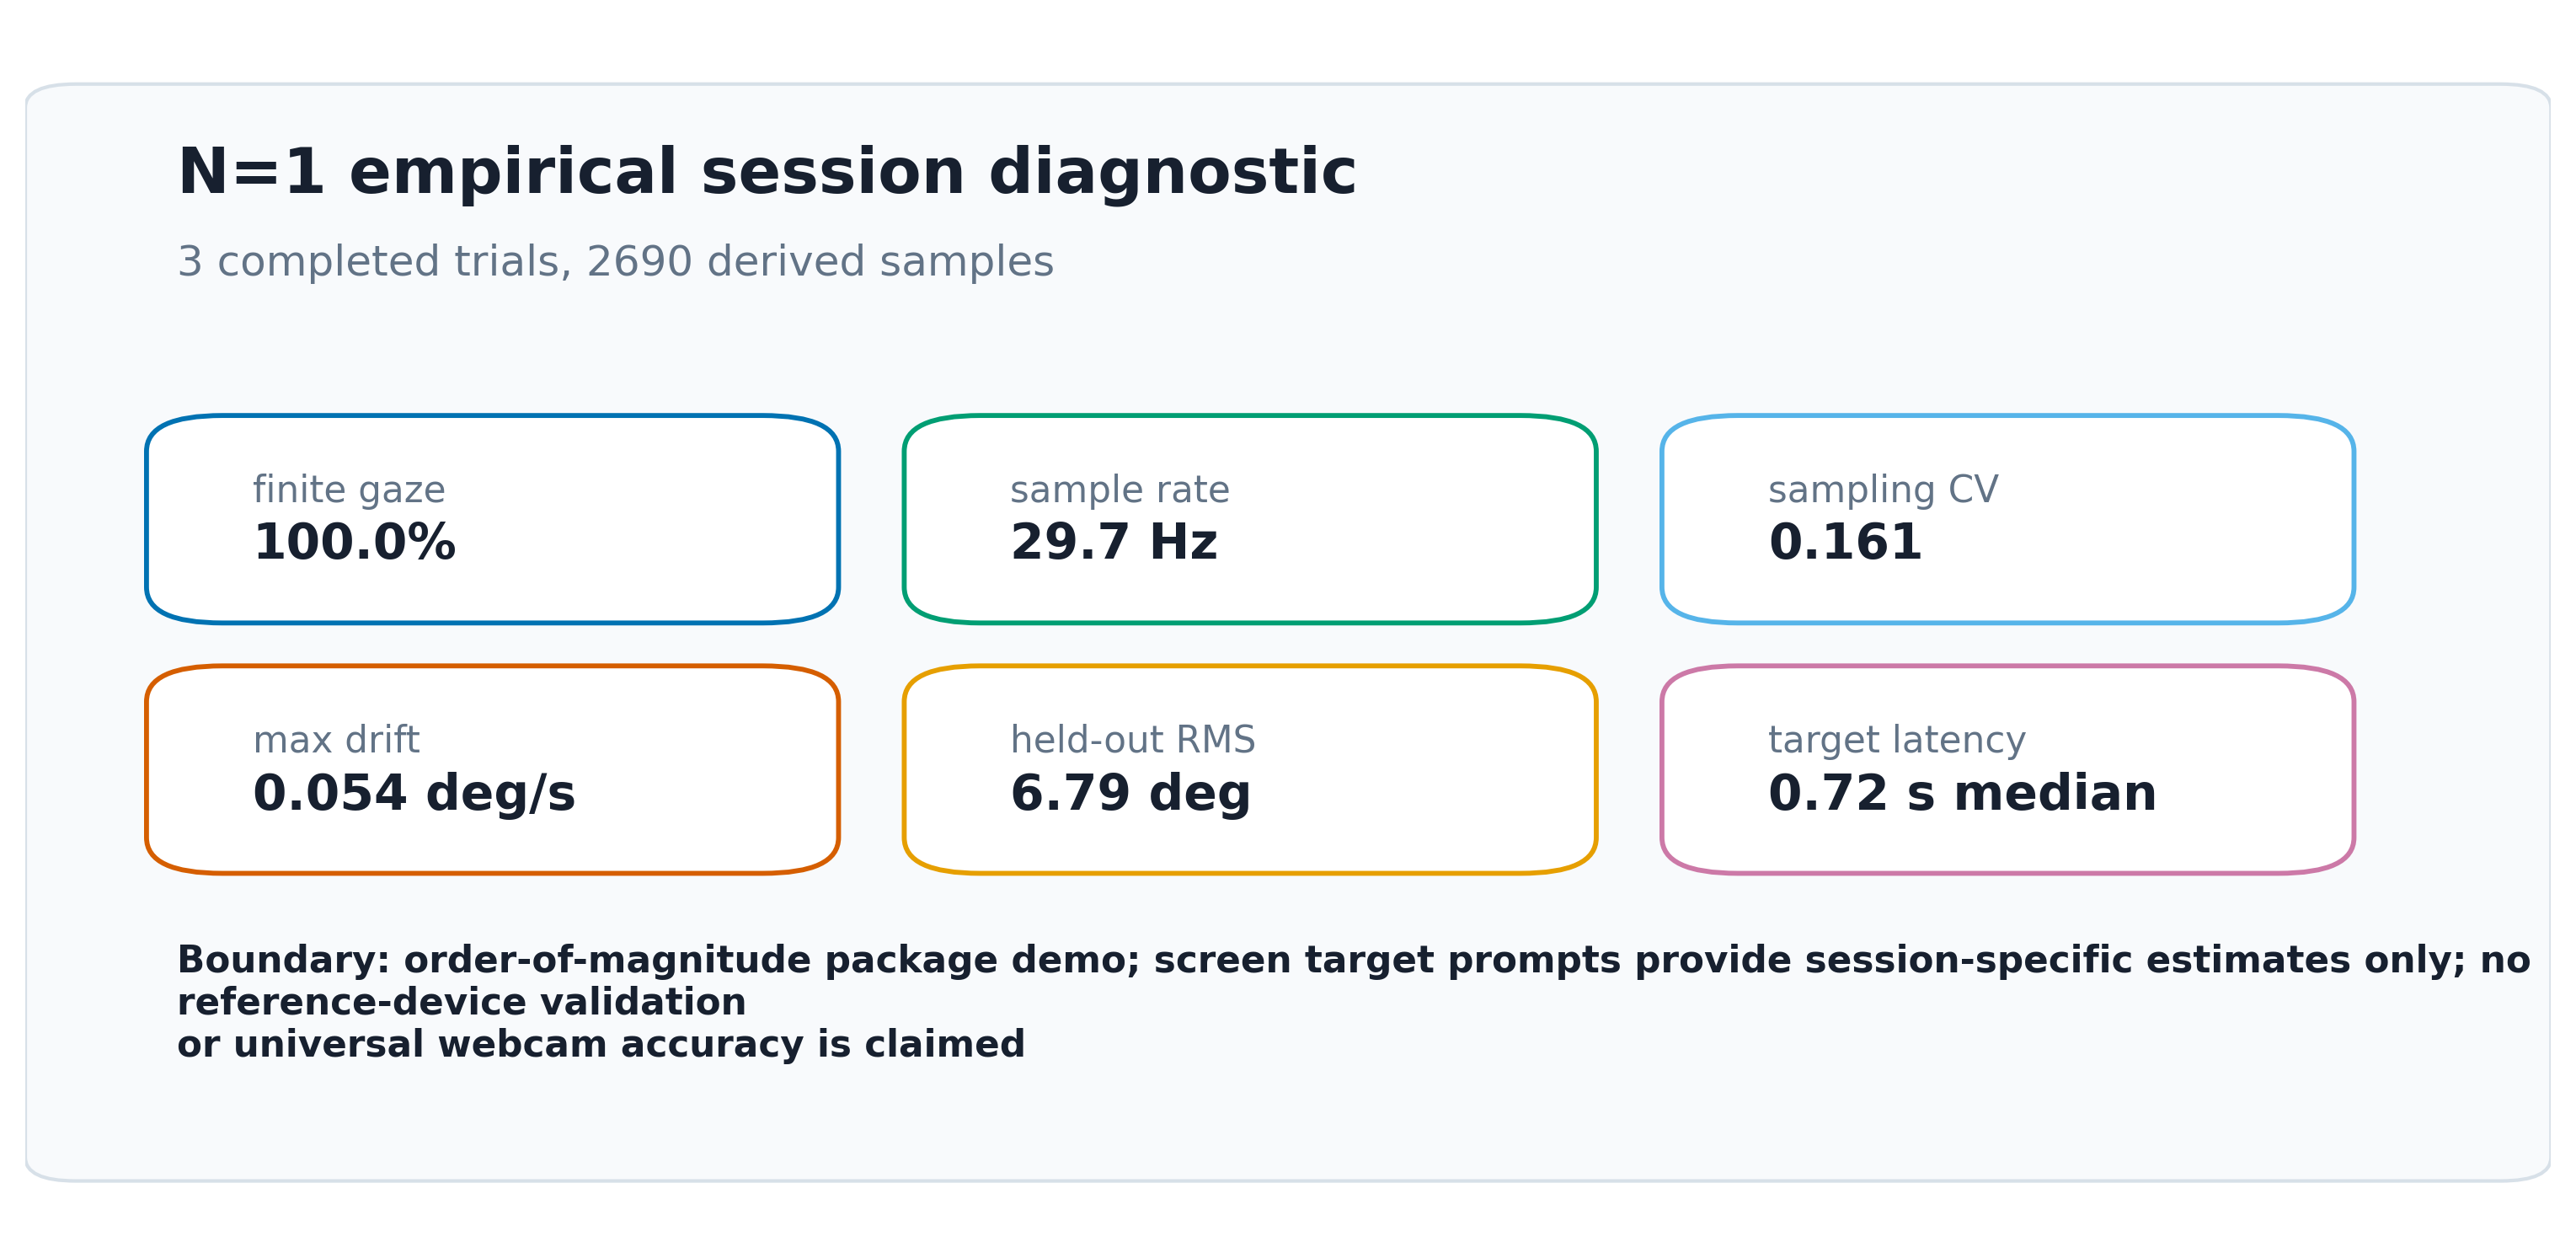
\includegraphics[width=1\linewidth,height=\textheight,keepaspectratio,alt={N=1 empirical session summary generated from the derived experiment report. The cards report finite-gaze fraction, sampling rate, sampling regularity, drift, held-out target residuals, and target acquisition latency as order-of-magnitude session diagnostics when a local pilot export exists; pending fields remain visible before recording. The figure demonstrates the package workflow and current-session quality ledger, not reference-device validation.}]{../output/figures/empirical_pilot_summary.png}
\caption{N=1 empirical session summary generated from the derived
experiment report. The cards report finite-gaze fraction, sampling rate,
sampling regularity, drift, held-out target residuals, and target
acquisition latency as order-of-magnitude session diagnostics when a
local pilot export exists; pending fields remain visible before
recording. The figure demonstrates the package workflow and
current-session quality ledger, not reference-device
validation.}\label{fig:empirical-pilot}
\end{figure}

For adding more data, the release path now uses
\texttt{docs/empirical\_sessions\_manifest.json} as an intake ledger.
Each available session must name the de-identified participant, device,
session group, replicate identifier, condition, protocol, consent scope,
reference-evidence type, and repo-relative derived report path; planned
sessions can be listed before their exports exist. A non-\texttt{none}
reference-evidence type counts only when the row also names a valid
repo-relative \texttt{reference\_artifact} JSON; for the
manual-annotation lane, that artifact stores sampled target-window
judgments over derived report/record files rather than raw video.

The v1 empirical release is intentionally scoped as a
single-participant, single-device, five-session diagnostic pilot, not as
a device-validation study. The generated
\texttt{docs/empirical\_sessions\_summary.json} and
fig.~\ref{fig:empirical-sessions-summary} therefore treat
participant/device counts as scope metadata while using five available
sessions, five replicate IDs, and the two collected lighting conditions
as the diagnostic readiness criteria. The current ledger reports
\textbf{5 available sessions, 5 replicate IDs, 2 conditions, 0
reference-backed rows} and is \textbf{ready for diagnostic v1}. Under
those checked-in diagnostic criteria, the minimum additional collection
needed for v1 is \textbf{0} additional session exports, with \textbf{0}
additional current-v1 condition(s) required.

The stronger 12-session, three-condition, reference-backed validation
plan is preserved as future scope rather than counted as a current v1
blocker: \textbf{7 future session exports, 1 future condition (missing:
indoor\_office\_backlit), and validated reference evidence still
required}. Prompt-only replicates improve within-participant/device
operating-scale coverage, but device validation still requires
reference-device, public-dataset, or manual-annotation evidence backed
by a valid artifact.

\begin{figure}
\centering
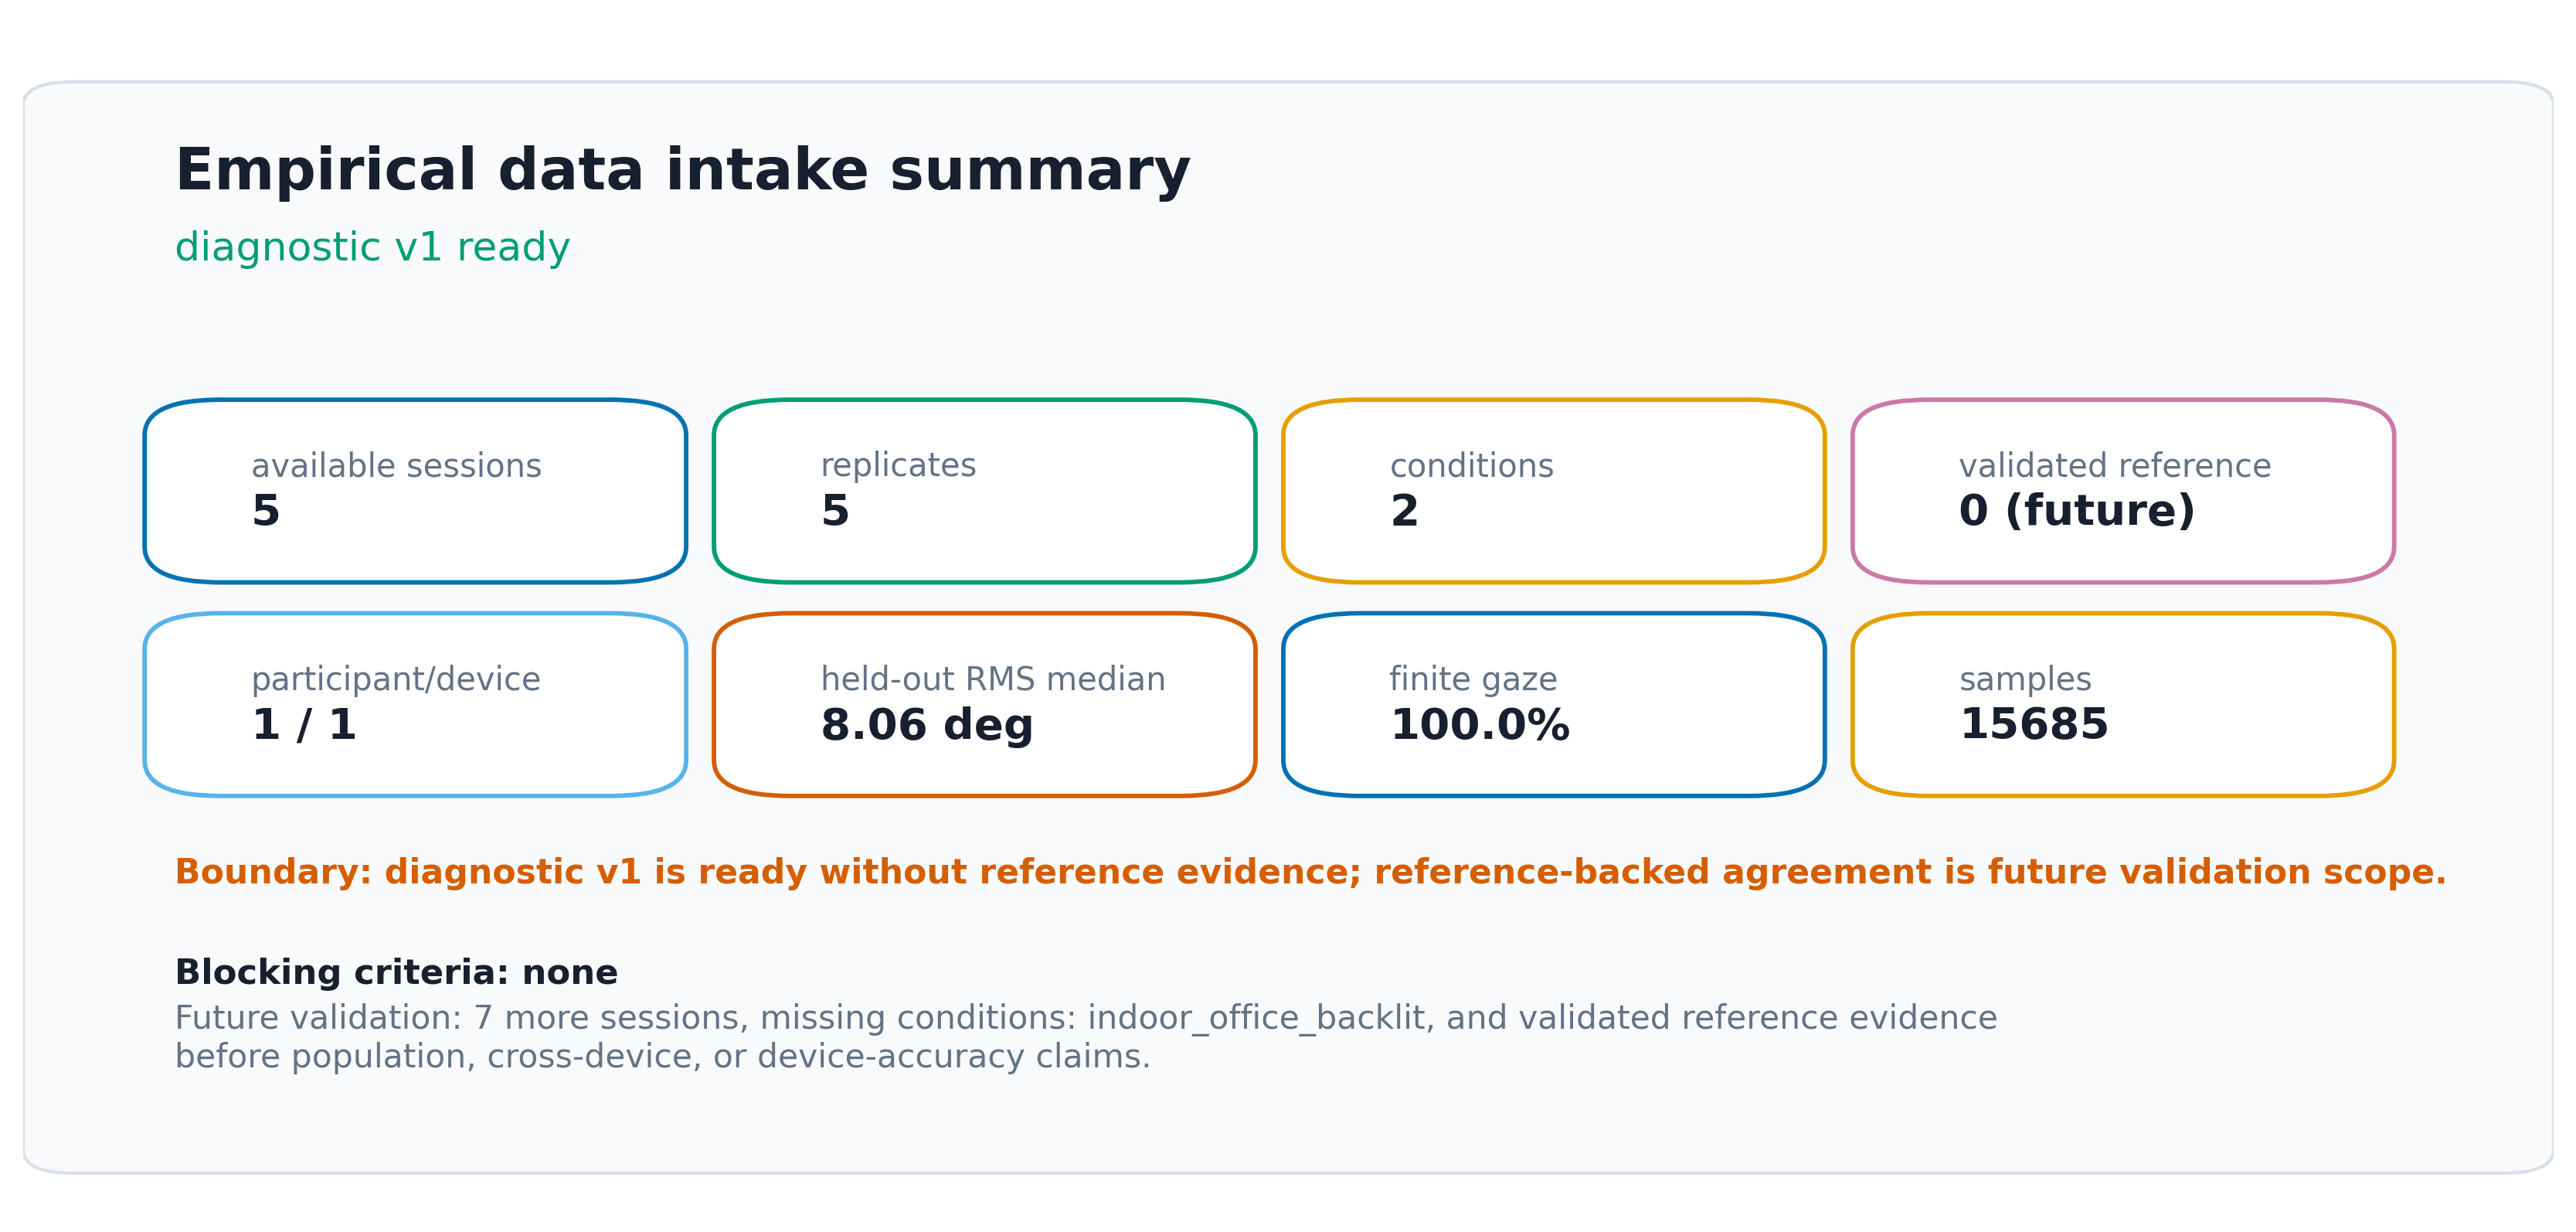
\includegraphics[width=1\linewidth,height=\textheight,keepaspectratio,alt={Empirical-session intake summary generated from docs/empirical\_sessions\_manifest.json. The figure reports available sessions, distinct replicates, conditions, reference-evidence count, participant/device scope, held-out residual scale, finite-gaze fraction, total derived samples, and current diagnostic-v1 status. The five-session prompt-only ledger is sufficient for diagnostic v1 readiness while population, cross-device, and device-accuracy claims remain future reference-backed validation scope.}]{../output/figures/empirical_sessions_summary.png}
\caption{Empirical-session intake summary generated from
\protect\texttt{docs/empirical\_sessions\_manifest.json}. The figure
reports available sessions, distinct replicates, conditions,
reference-evidence count, participant/device scope, held-out residual
scale, finite-gaze fraction, total derived samples, and current
diagnostic-v1 status. The five-session prompt-only ledger is sufficient
for diagnostic v1 readiness while population, cross-device, and
device-accuracy claims remain future reference-backed validation
scope.}\label{fig:empirical-sessions-summary}
\end{figure}

The pilot adds a different kind of evidence from the synthetic results.
Synthetic truth recovery and the 3-D closed loop test the estimator
under known gaze, events, and geometry (sec.~\ref{sec:results};
sec.~\ref{sec:closedloop}); the noise sweep then shows how idealised
landmark jitter propagates through the real estimator
(sec.~\ref{sec:noiseresults}). The single local run instead
contextualizes the scale of one real session: finite capture, webcam
sampling regularity, short-session drift, prompted-target residuals, and
UI/capture target acquisition latency. In that interpretation, the
finite-gaze fraction and sampling CV are capture-stability checks, the
drift value is a short-session stability check, the held-out RMS is a
prompted-target residual scale, and the latency is a coarse task/UI
timing quantity. None of these should be read as physiological saccade
latency or reference-device gaze accuracy.

The pilot therefore sanity-checks one local operating scale for
synthetic data generation without turning those variables into measured
population parameters. The comparison is deliberately coarse, and
fig.~\ref{fig:synthetic-empirical-range-bridge} renders the same
comparison from a generated JSON sidecar so the visual and prose share
one evidence boundary:

\begin{longtable}[]{@{}
  >{\raggedright\arraybackslash}p{(\linewidth - 6\tabcolsep) * \real{0.2308}}
  >{\raggedleft\arraybackslash}p{(\linewidth - 6\tabcolsep) * \real{0.3077}}
  >{\raggedright\arraybackslash}p{(\linewidth - 6\tabcolsep) * \real{0.2308}}
  >{\raggedright\arraybackslash}p{(\linewidth - 6\tabcolsep) * \real{0.2308}}@{}}
\caption{N=1 pilot scale compared with synthetic/model
variables.}\label{tbl:empirical-synthetic-range}\tabularnewline
\toprule\noalign{}
\begin{minipage}[b]{\linewidth}\raggedright
Pilot diagnostic
\end{minipage} & \begin{minipage}[b]{\linewidth}\raggedleft
Hydrated value
\end{minipage} & \begin{minipage}[b]{\linewidth}\raggedright
Context
\end{minipage} & \begin{minipage}[b]{\linewidth}\raggedright
Range interpretation
\end{minipage} \\
\midrule\noalign{}
\endfirsthead
\toprule\noalign{}
\begin{minipage}[b]{\linewidth}\raggedright
Pilot diagnostic
\end{minipage} & \begin{minipage}[b]{\linewidth}\raggedleft
Hydrated value
\end{minipage} & \begin{minipage}[b]{\linewidth}\raggedright
Context
\end{minipage} & \begin{minipage}[b]{\linewidth}\raggedright
Range interpretation
\end{minipage} \\
\midrule\noalign{}
\endhead
\bottomrule\noalign{}
\endlastfoot
Finite gaze & 100.0\% & clean-session finite-sample examples; dropout
domains & Supports the clean synthetic demos as plausible for a
cooperative local run, while preserving low-light/dropout stress
cases. \\
Sampling rate & 29.7 Hz & live-style sampling cadence and timestamp grid
& Contextualizes webcam-rate synthetic/session examples near a
consumer-camera cadence rather than the higher-rate ideal traces used
for algorithmic recovery. \\
Sampling CV & 0.161 & timestamp jitter in synthetic sessions & Gives an
order-of-magnitude jitter target for live-style stress tests, separate
from deterministic oracle traces. \\
Maximum drift & 0.054 deg/s & head-drift and fixation-stability domains
& Supports a low-drift baseline example; larger drift domains remain
stress tests, not observed claims from this pilot. \\
Held-out target RMS & 6.79 deg & prompted-target residual /
calibration-bias scale & Contextualizes screen-prompt and calibration
residual scale; it is not iid landmark noise, closed-loop residual, or
gaze accuracy against a reference device. \\
Target acquisition latency & 0.72 s median & target-schedule and
UI/capture timing & Contextualizes task-response timing for the live
protocol; it is not physiological saccade latency. \\
\end{longtable}

\begin{figure}
\centering
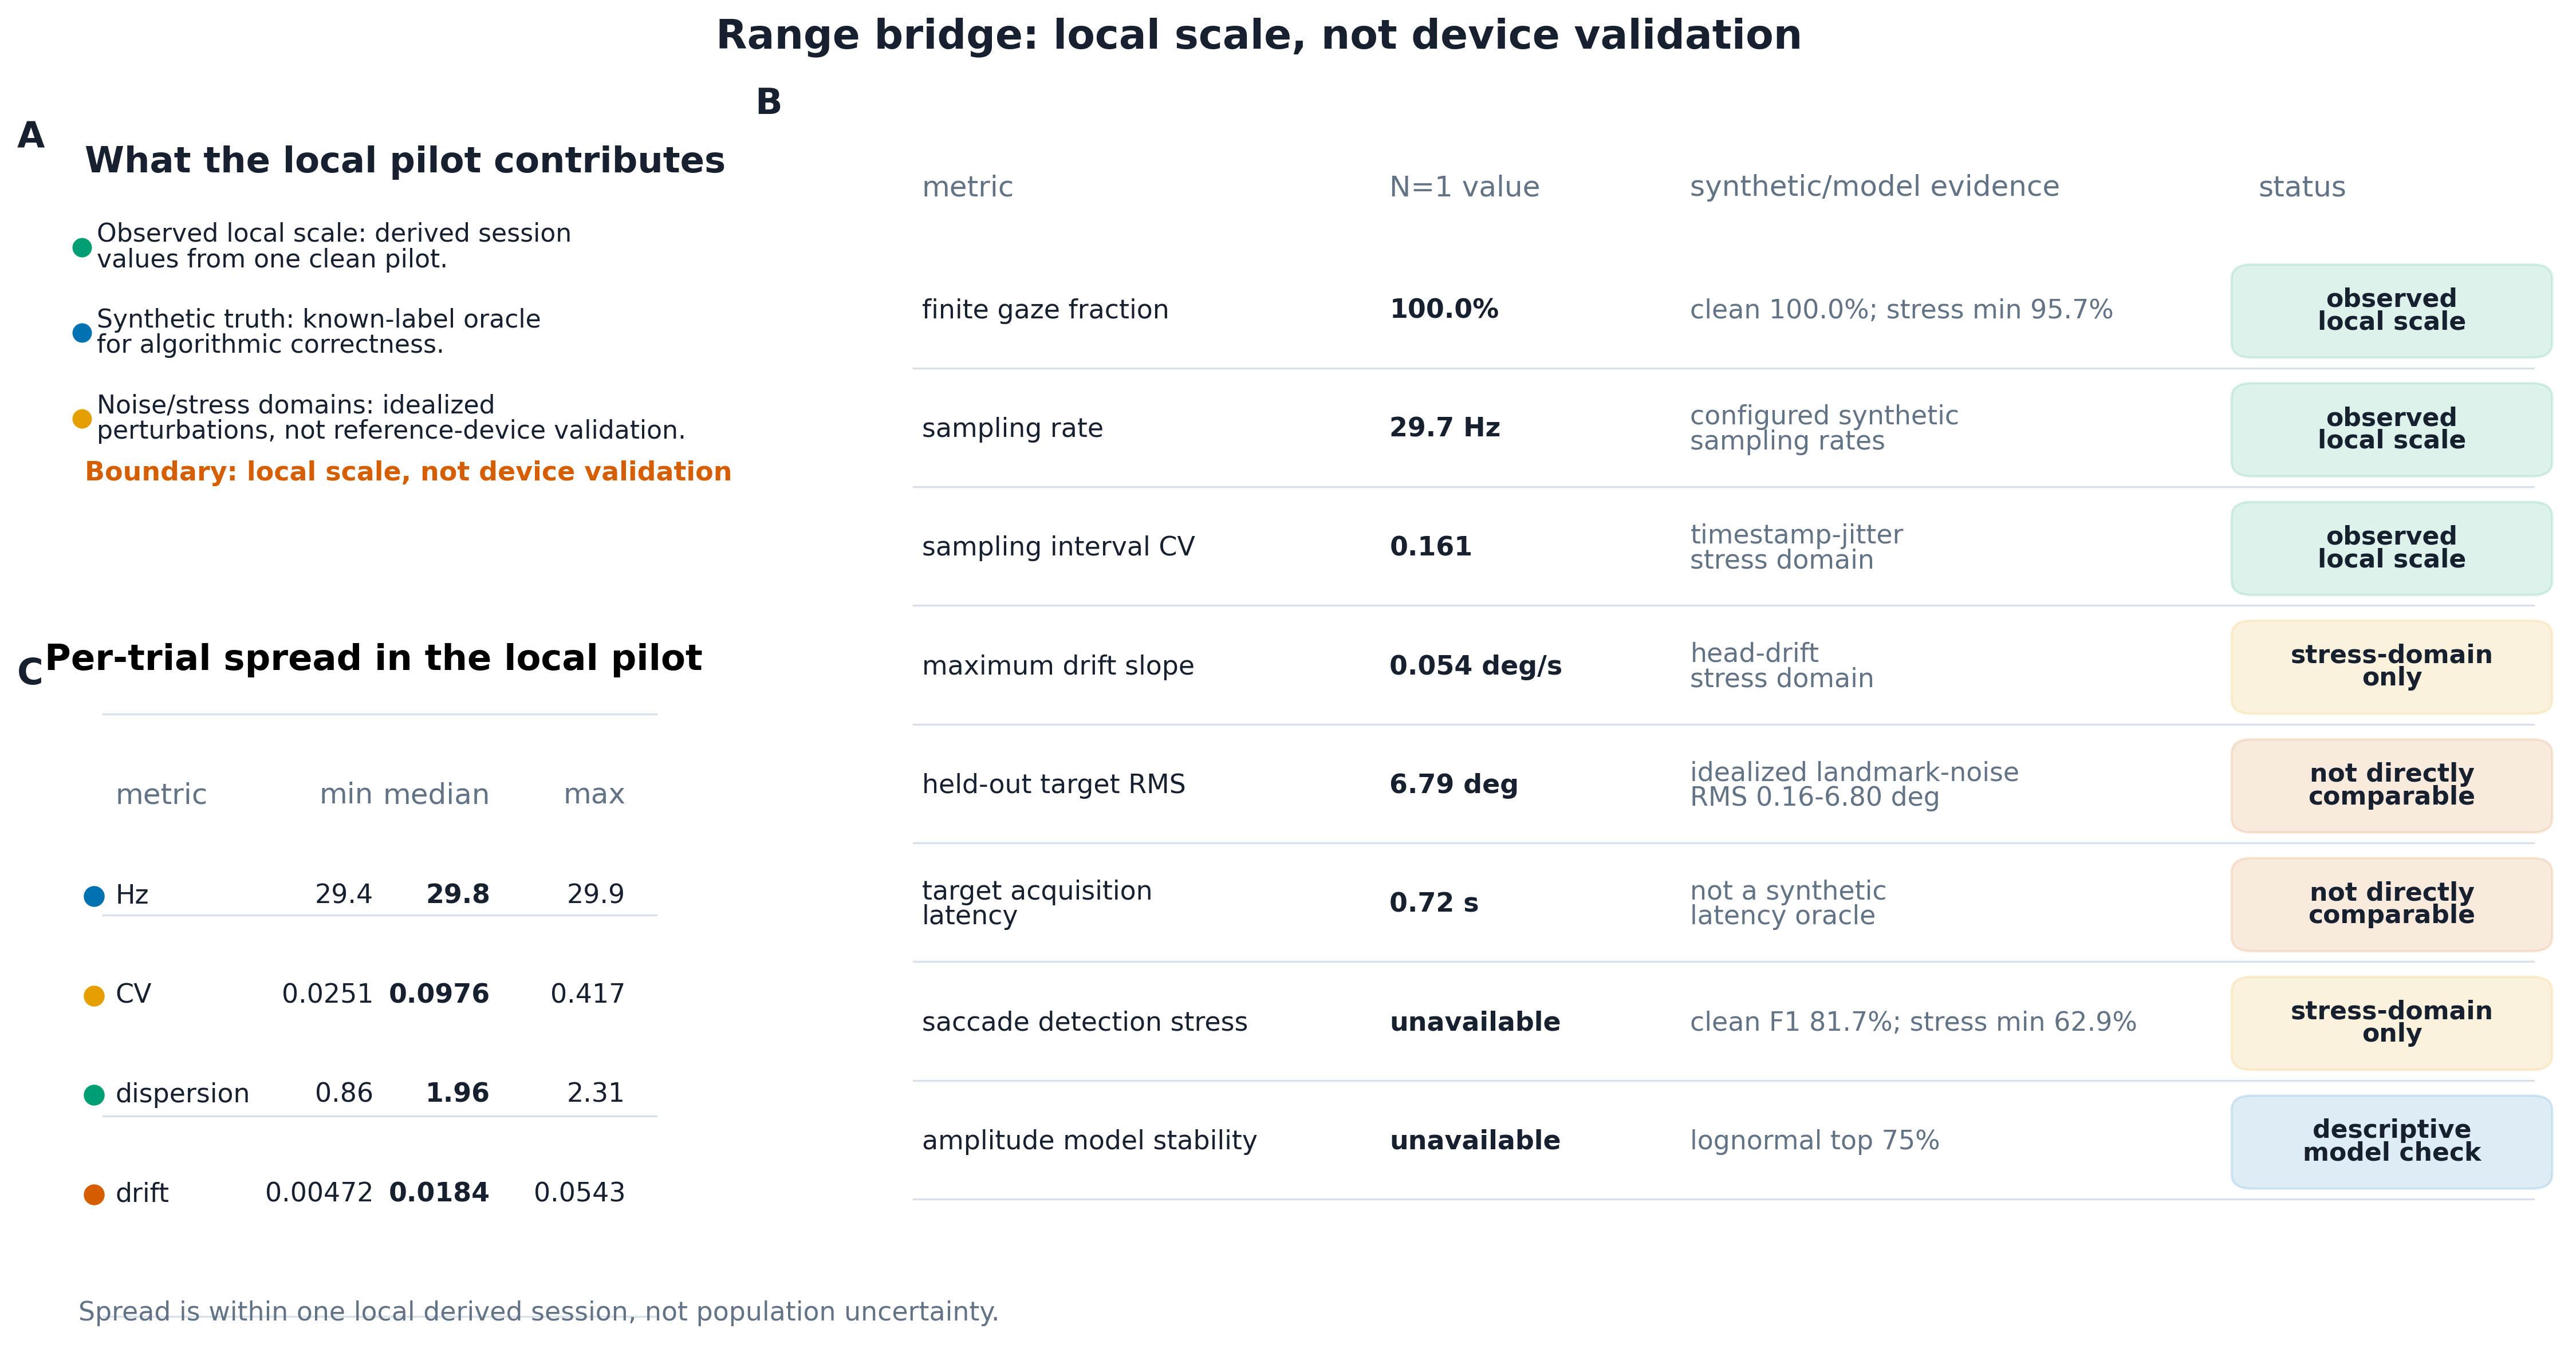
\includegraphics[width=1\linewidth,height=\textheight,keepaspectratio,alt={Synthetic-to-empirical range bridge generated from output/figures/synthetic\_empirical\_range\_bridge.json. The rows place N=1 empirical session values beside synthetic-domain summaries, idealized landmark-noise sweep values, or descriptive statistical diagnostics, and each row is labelled as observed local scale, stress-domain only, or not directly comparable. The figure uses the pilot to contextualize synthetic defaults and stress ranges; it does not validate device accuracy, device performance, or webcam generality.}]{../output/figures/synthetic_empirical_range_bridge.png}
\caption{Synthetic-to-empirical range bridge generated from
\protect\texttt{output/figures/synthetic\_empirical\_range\_bridge.json}.
The rows place N=1 empirical session values beside synthetic-domain
summaries, idealized landmark-noise sweep values, or descriptive
statistical diagnostics, and each row is labelled as observed local
scale, stress-domain only, or not directly comparable. The figure uses
the pilot to contextualize synthetic defaults and stress ranges; it does
not validate device accuracy, device performance, or webcam
generality.}\label{fig:synthetic-empirical-range-bridge}
\end{figure}

This comparison is intentionally asymmetric. The synthetic closed loop
reports a near-ideal residual because both truth and measurements are
generated inside a controlled model, while the N=1 pilot folds in
calibration quality, user compliance, webcam timing, landmark behaviour,
screen geometry, and target eccentricity. A much larger prompted-target
RMS in fig.~\ref{fig:synthetic-empirical-range-bridge} is therefore not
a contradiction of the synthetic validation; it is the practical scale
at which the package's live workflow operates before any reference
tracker is introduced. That makes the pilot useful for choosing
realistic demo defaults, stress-test ranges, and caveats, while leaving
real-device validation to a future public-dataset or reference-device
study.

\section{Results: figure gallery}\label{sec:gallery}

The analysis core is paired with a deterministic visualization layer
(\texttt{itrace.viz}, matplotlib on the headless Agg backend) that
renders the standard eye-movement figures directly from a
\texttt{SessionReport}. Each figure is produced from a synthetic session
whose ground truth is known by construction, so the gallery is
reproducible byte-for-byte and never depends on a captured recording.
Categorical series draw from the shared Wong (2011) colour-blind-safe
palette; scalar fields use perceptual sequential or diverging colormaps
that match the quantity being encoded. All panels share the same house
style --- a readable font floor, white background, restrained spines,
and compact result callouts --- so the published figures match without
pretending one palette serves every data type. In the multi-series
comparison figures, signals are separated by marker and line style as
well as colour, so the figures stay legible in greyscale. The figures
below are regenerated for publication by
\texttt{scripts/generate\_figures.py}, which also writes the graphical
abstract, noise sidecars, empirical summary, and figure manifest. The
CLI command
\texttt{itrace\ figures\ -\/-out-dir\ output/figures\ -\/-animations}
remains the gallery-only refresh path.

The gallery spans the three signal families iTrace recovers. For
\textbf{gaze and events}, a velocity trace
(\texttt{output/figures/velocity\_trace.png}) overlays the 2-D speed
signal with the I-VT threshold and shades each detected saccade, while a
spatial scanpath (\texttt{output/figures/scanpath.png}) draws fixations
sized by dwell time and joined by fixation-transition arrows in screen
coordinates. For \textbf{saccade dynamics}, an amplitude histogram
(\texttt{output/figures/amplitude\_histogram.png}) carries its
maximum-likelihood distribution overlay, and a main-sequence panel
(\texttt{output/figures/main\_sequence\_diagnostics.png}) plots
amplitude against peak velocity on log-log axes with the fitted power
law and its residuals. For \textbf{pupillometry}, a pupil trace
(\texttt{output/figures/pupil\_trace.png}) shows the raw signal, the
blink-interpolated and smoothed overlay, and the causally-detected
dilation peaks and troughs.

A multi-panel session dashboard
(\texttt{output/figures/session\_dashboard.png}) composes the velocity
trace, scanpath, amplitude distribution, main sequence,
saccade-direction polar histogram, and a textual summary into a single
at-a-glance figure. The statistical diagnostics composite in
fig.~\ref{fig:statistical-diagnostics} takes the same
\texttt{SessionReport} view and makes the statistics layer inspectable:
distribution-family ranking is plotted as lower-is-better AIC deltas
with AIC weights, AICc, BIC/KS annotations, and robust amplitude-shape
fields (median and IQR with seeded bootstrap intervals, Bowley skewness,
and IQR outside values), plus a seeded bootstrap of the lowest-AIC
family winner to show model-ranking stability without treating that
frequency as a posterior probability. The best-fit amplitude family is
checked against empirical quantiles and fitted-CDF residuals with
integrated/tail-weighted distance summaries and a DKW/Massart reference
band, the main-sequence exponent is shown with a seeded bootstrap
interval, fixation centroids are paired with dispersion/BCEA/hull
descriptors, and the scanpath string is decomposed into a first-order
transition matrix. The panel is useful because each plotted value is
computed by the tested Python statistics modules; it does not turn a
synthetic session into population physiology or device validation
evidence. The same refresh writes
\texttt{output/figures/statistical\_diagnostics.json}, so the PNG is
display-only over an audited statistical payload rather than an
untracked matplotlib-only calculation.

\begin{figure}
\centering
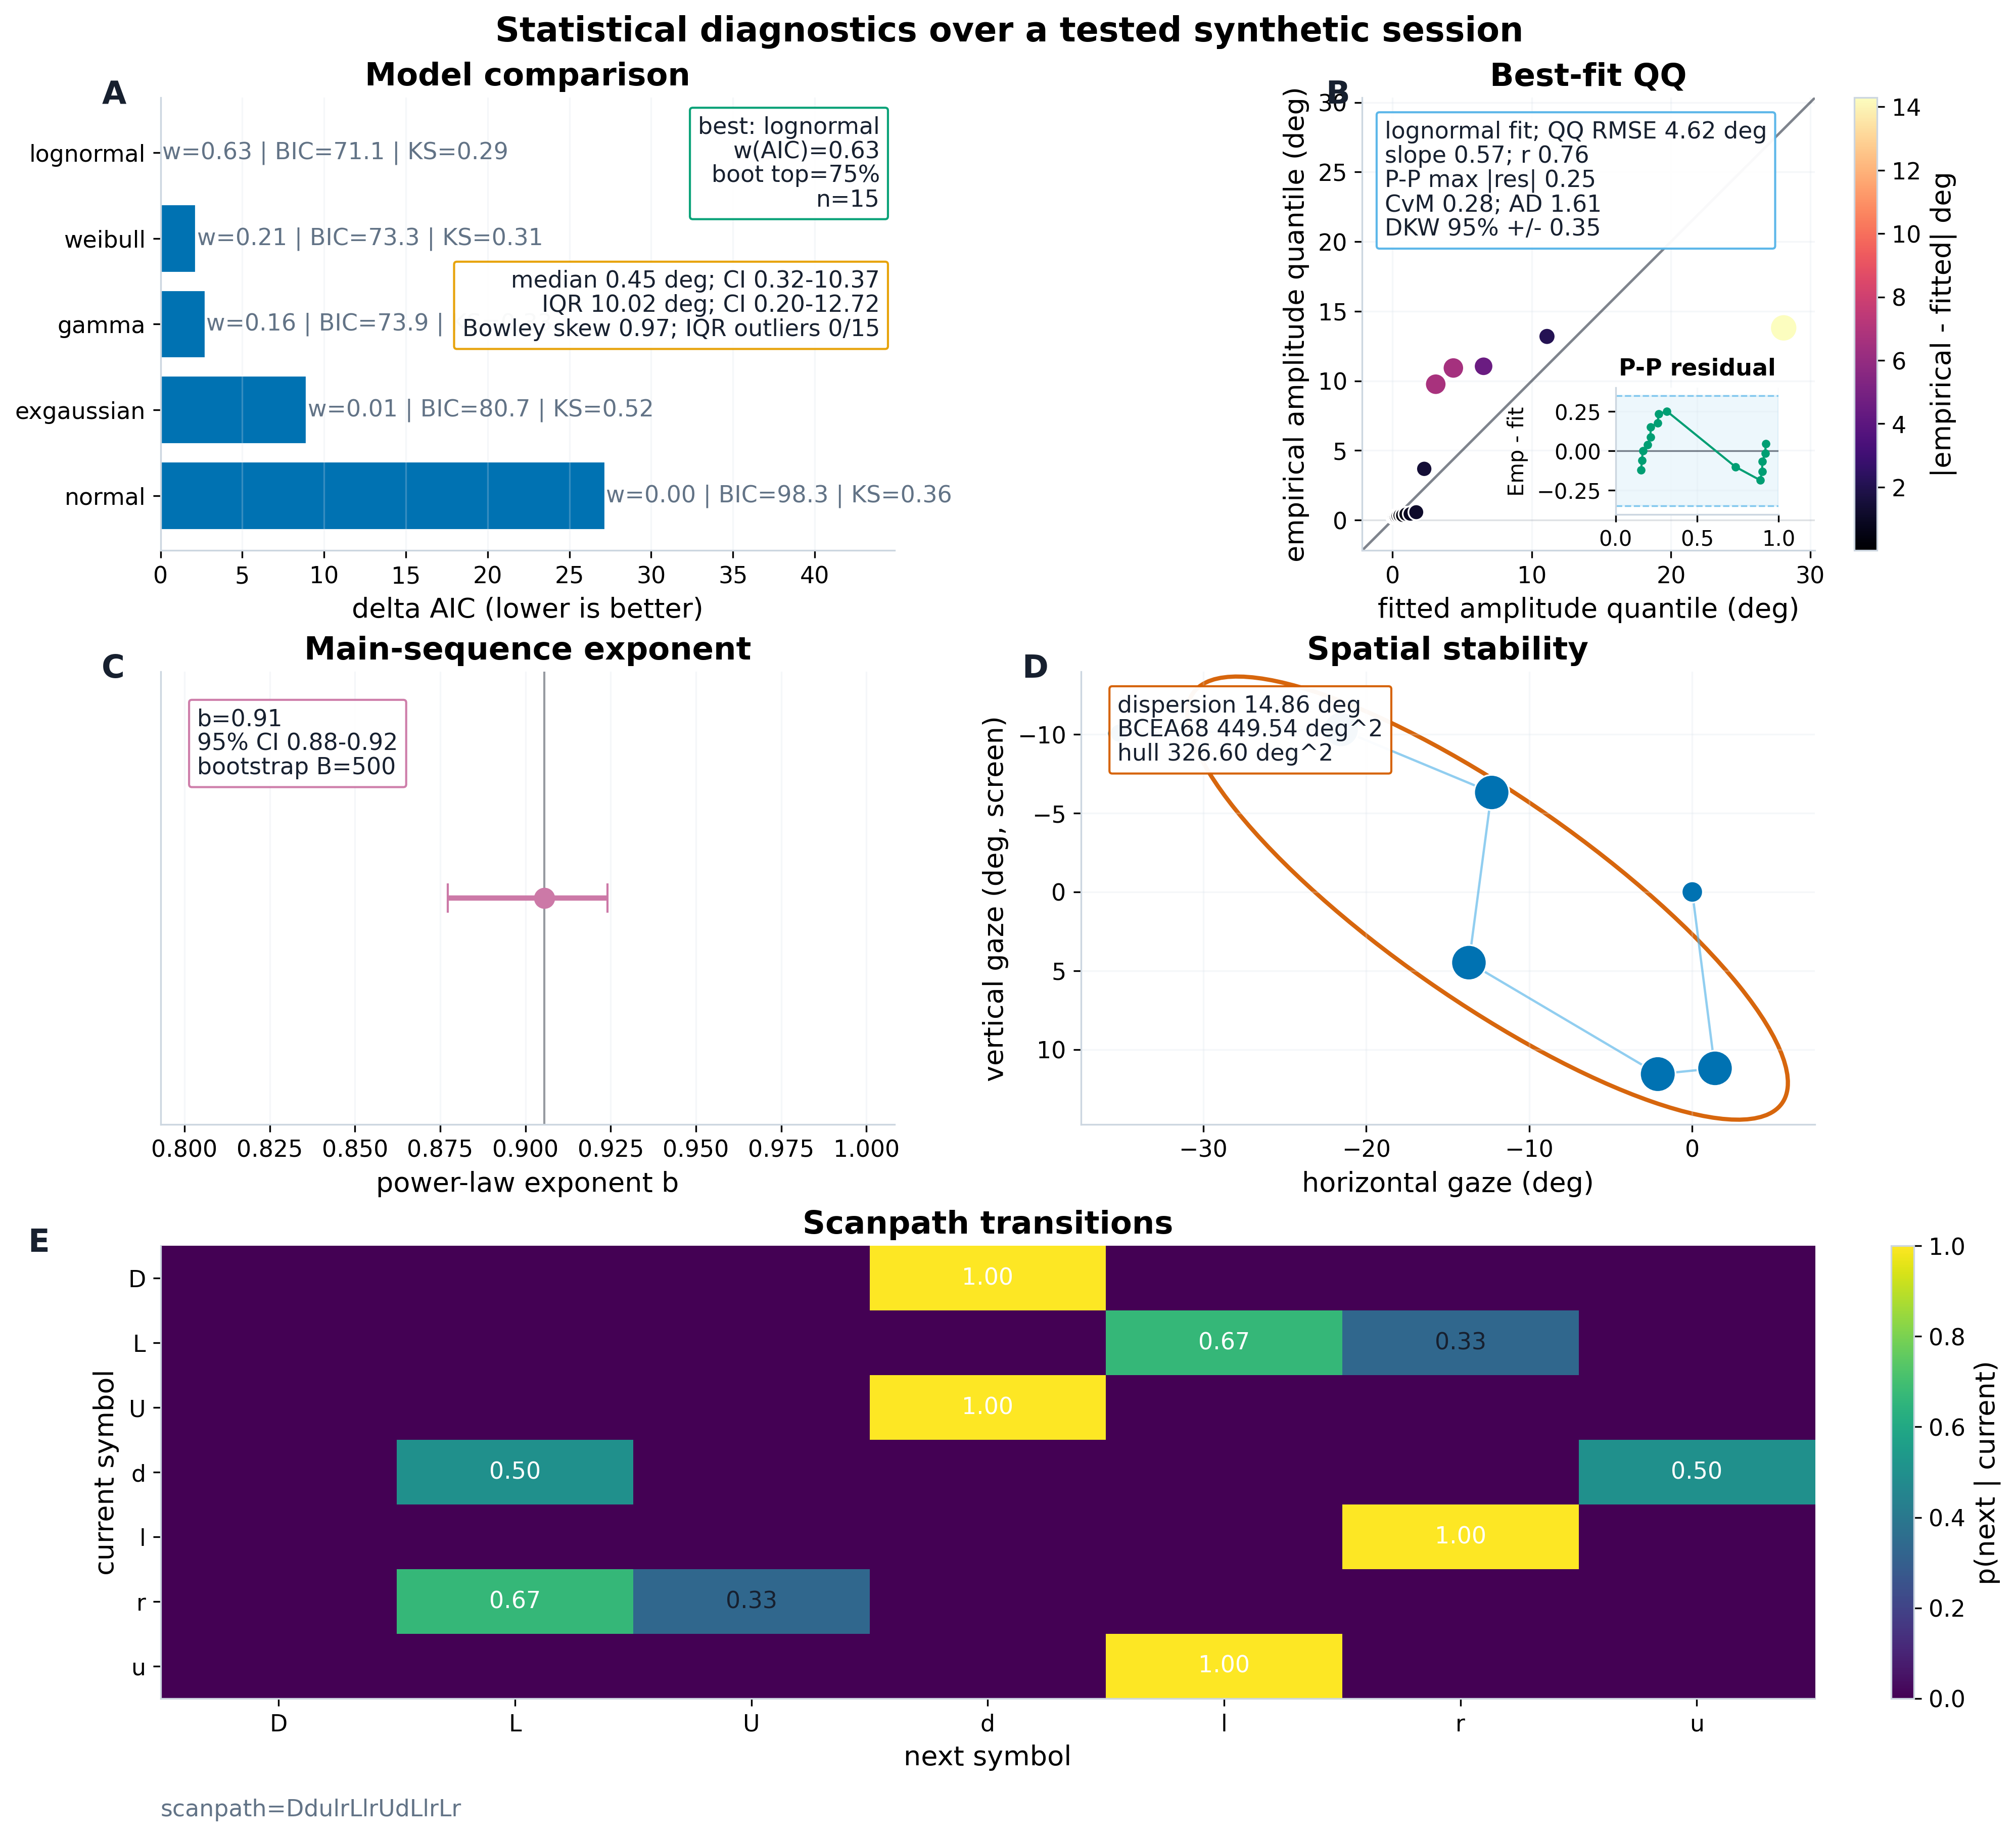
\includegraphics[width=1\linewidth,height=\textheight,keepaspectratio,alt={Statistical diagnostics over a deterministic synthetic session. Panel A ranks amplitude-distribution families by delta AIC while carrying Akaike weights, AICc, BIC, Kolmogorov-Smirnov descriptors, bootstrap lowest-AIC winner stability, robust median/IQR shape summaries with seeded bootstrap intervals, Bowley quartile skewness, and IQR outside-value counts; panel B plots empirical amplitude quantiles against fitted quantiles for the lowest-AIC family, reports QQ residual scale, and adds a P-P/CDF residual inset with integrated and Anderson-Darling-style tail-weighted CDF distances plus a DKW/Massart reference band; panel C shows the seeded bootstrap interval for the main-sequence exponent; panel D overlays fixation centroids with a BCEA-style ellipse and spatial-spread summaries; panel E renders the row-normalised scanpath transition matrix. The figure visualizes tested core descriptors and relative model diagnostics, not real-eye accuracy, population inference, or proof that a fitted family is true.}]{../output/figures/statistical_diagnostics.png}
\caption{Statistical diagnostics over a deterministic synthetic session.
Panel A ranks amplitude-distribution families by delta AIC while
carrying Akaike weights, AICc, BIC, Kolmogorov-Smirnov descriptors,
bootstrap lowest-AIC winner stability, robust median/IQR shape summaries
with seeded bootstrap intervals, Bowley quartile skewness, and IQR
outside-value counts; panel B plots empirical amplitude quantiles
against fitted quantiles for the lowest-AIC family, reports QQ residual
scale, and adds a P-P/CDF residual inset with integrated and
Anderson-Darling-style tail-weighted CDF distances plus a DKW/Massart
reference band; panel C shows the seeded bootstrap interval for the
main-sequence exponent; panel D overlays fixation centroids with a
BCEA-style ellipse and spatial-spread summaries; panel E renders the
row-normalised scanpath transition matrix. The figure visualizes tested
core descriptors and relative model diagnostics, not real-eye accuracy,
population inference, or proof that a fitted family is
true.}\label{fig:statistical-diagnostics}
\end{figure}

The statistical panel is intentionally information-dense, so
fig.~\ref{fig:statistical-interpretation-ledger} records the companion
interpretation ledger generated from
\texttt{output/figures/statistical\_interpretation\_ledger.json}. Each
row names the statistic, its reported value, the estimand it actually
summarizes, and the claim it explicitly does not support. This matters
for the scholarship boundary: AIC weights remain relative
candidate-family weights, DKW bands remain finite-sample empirical-CDF
reference bands, bootstrap intervals remain report-level uncertainty
summaries, and the N=1 range bridge remains a single-session scale check
rather than device validation.

\begin{figure}
\centering
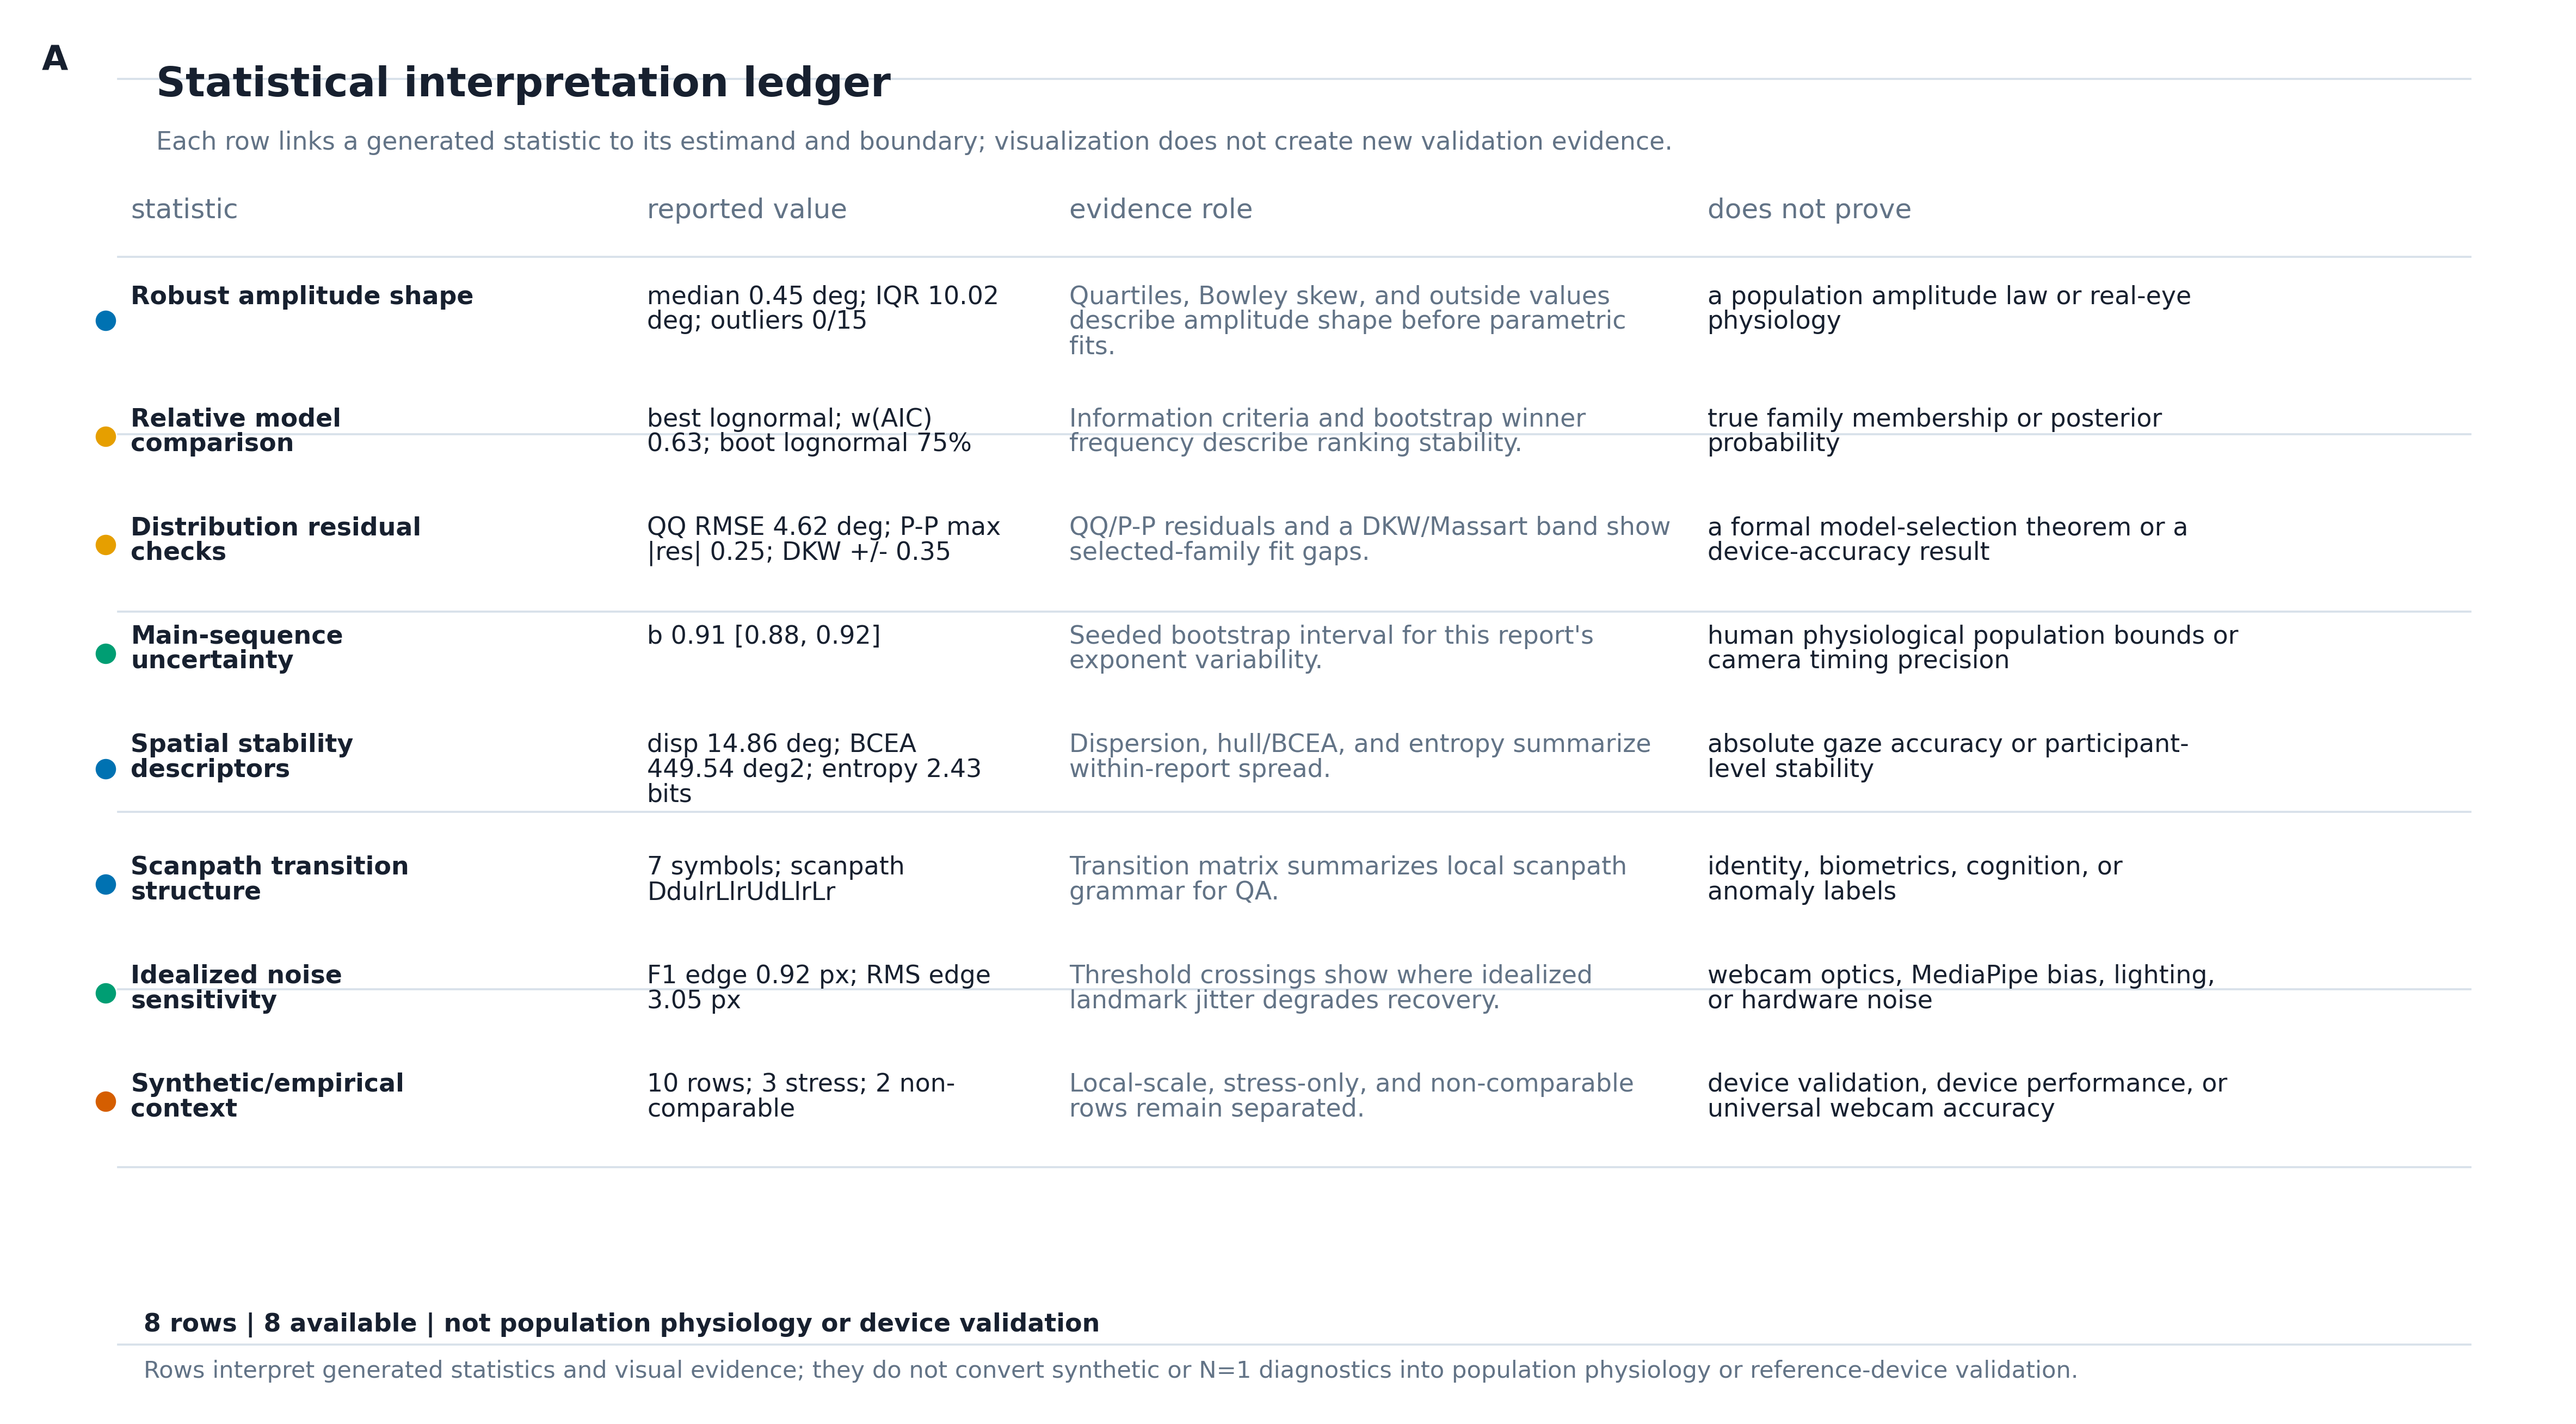
\includegraphics[width=1\linewidth,height=\textheight,keepaspectratio,alt={Statistical interpretation ledger generated from output/figures/statistical\_interpretation\_ledger.json. The rows map robust shape summaries, relative distribution comparison, CDF residual checks, bootstrap main-sequence uncertainty, spatial descriptors, scanpath transitions, idealized noise sensitivity, and the synthetic-to-empirical range bridge to their source artifacts, estimands, and explicit non-claims. The figure improves statistical readability without adding new evidence; it states what each statistic does not prove, including population physiology, posterior model truth, real-eye accuracy, and device validation.}]{../output/figures/statistical_interpretation_ledger.png}
\caption{Statistical interpretation ledger generated from
\protect\texttt{output/figures/statistical\_interpretation\_ledger.json}.
The rows map robust shape summaries, relative distribution comparison,
CDF residual checks, bootstrap main-sequence uncertainty, spatial
descriptors, scanpath transitions, idealized noise sensitivity, and the
synthetic-to-empirical range bridge to their source artifacts,
estimands, and explicit non-claims. The figure improves statistical
readability without adding new evidence; it states what each statistic
does not prove, including population physiology, posterior model truth,
real-eye accuracy, and device
validation.}\label{fig:statistical-interpretation-ledger}
\end{figure}

The gallery now also includes gaze density, fixation heatmap, AOI dwell,
event raster, pupil PSD, saccade-rate, microsaccade, and deterministic
synthetic replay outputs. Because every panel is a pure function of a
\texttt{SessionReport}, the same plots apply unchanged to a real
recording analysed through the pipeline, subject to the same detector
and calibration limits stated in sec.~\ref{sec:limitations}.

\section{Results: scanpath comparison and temporal
dynamics}\label{sec:scanresults}

The descriptive scanpath metrics of sec.~\ref{sec:diststats} and the
spatial/timeline visualisations of sec.~\ref{sec:gallery} turn a single
recording into a comparable summary of \emph{where} and \emph{when} gaze
moved. As everywhere in this section, the inputs are synthetic sessions
with known ground truth: the numbers below are internal-consistency
checks on the metrics and detectors, not measurements of a real eye
(sec.~\ref{sec:limitations}).

\subsection{Self-similarity is a tautology, used as a
control}\label{self-similarity-is-a-tautology-used-as-a-control}

Comparing a synthetic session against an exact copy of itself returns a
similarity of 1.0, and comparing it against a deterministically
time-shifted copy returns the same value once the paths are aligned.
This is true \emph{by construction} --- identical fixation centroids and
saccade sequences cannot differ --- so it is reported not as a finding
but as the degenerate anchor every similarity measure must hit. Its
value is as a negative control: a measure that failed to return 1.0 on a
session against itself would be broken, and perturbing one fixation by a
known offset drops the similarity below 1.0 in the expected direction,
confirming the measure responds to real differences rather than always
saturating.

\subsection{Adaptive and fixed thresholds recover the same scripted
events}\label{adaptive-and-fixed-thresholds-recover-the-same-scripted-events}

The scripted multi-saccade sessions are built so that fixed-threshold
I-VT (\citeproc{ref-salvucci2000identifying}{Salvucci and Goldberg
2000}) and a data-adaptive threshold derived from the velocity
distribution (\citeproc{ref-nystrom2010adaptive}{Nyström and Holmqvist
2010}) should classify the same intervals. They do: on the synthetic
grid both recover the same saccade count with onsets agreeing to within
a sample, and the adaptive threshold settles inside the band of fixed
thresholds that bracket the clean velocity gap. Where the signal carries
injected noise the two diverge first on the smallest events, the same
fragility that the saccade-F1 collapse of sec.~\ref{sec:noiseresults}
makes quantitative. The point is a cross-check between two independent
detector designs on a shared, known-truth signal --- the kind of
agreement an event-classification reference implementation is meant to
provide (\citeproc{ref-dar2021remodnav}{Dar et al. 2021}) --- not a
claim that either threshold is correct for real webcam data.

\subsection{Windowed event rates expose temporal
structure}\label{windowed-event-rates-expose-temporal-structure}

Sliding a fixed-width window across a session and counting events per
window yields a saccade-rate and fixation-rate time series whose
envelope tracks the scripted event schedule: rate peaks line up with the
constructed saccade bursts and fall to zero across the long fixations,
and integrating the windowed counts recovers the total event counts of
the whole-session report. The microsaccade rate over a fixational-jitter
session stays near zero except around the single injected microsaccade,
the temporal counterpart to the amplitude separation seen in
sec.~\ref{sec:results}. These windowed rates are descriptive summaries
of the detected event stream; on a synthetic session they recover the
schedule we wrote in, and on a real recording they would inherit exactly
the detector fragilities catalogued in sec.~\ref{sec:noiseresults}, with
no additional accuracy implied.

Taken together, the spatial spread metrics (dispersion, convex-hull
area, BCEA, and the two scanpath entropies of sec.~\ref{sec:diststats})
and the timeline views give a consistent, reproducible picture of the
synthetic sessions: structured scanpaths read as low
direction-transition entropy and a compact hull, diffuse ones as the
opposite, and the temporal rates localise each event in time. Every
number is a property of the detected events on a known-truth signal ---
a verification that the metrics and detectors behave as specified, kept
strictly separate from any claim about real-eye behaviour.

\section{Discussion}\label{sec:discussion}

\subsection{What the decoupling buys}\label{what-the-decoupling-buys}

By implementing established algorithms in a hardware-free core and
verifying them against constructed ground truth, iTrace makes the
scientific layer continuously testable and reproducible. A regression in
the saccade detector, the microsaccade threshold, or the blink
interpolation is caught by a headless test run, not discovered later on
real data. The optional capture shell can then evolve --- new landmark
backends, browser capture, deep-learning gaze --- without putting the
verified core at risk, because the shell only produces the gaze and
pupil streams the core already analyses. The local HTML orchestrator is
an example of this discipline: the browser receives eye crops and
plot-ready summaries, but all capture, estimation, event detection,
statistics, and export remain in the same Python package path tested
elsewhere. This is the central design message of
fig.~\ref{fig:graphical-abstract}: the camera path is an input shell,
while the evidence path is a reproducible sequence of typed records,
tested algorithms, and rendered reports.

\subsection{What the expanded analysis layer
adds}\label{what-the-expanded-analysis-layer-adds}

The same decoupling extends past detection into description. On top of
the estimators sits a quantitative layer (\texttt{itrace.stats}) and a
visualization layer (\texttt{itrace.viz}), both pure-core in spirit: the
statistics modules import only NumPy/SciPy, and matplotlib is confined
to the optional \texttt{figures} extra so the core stays headless. The
statistics layer turns the typed events of sec.~\ref{sec:events} and
sec.~\ref{sec:dynamics} into descriptive summaries of fixation and
saccade quantities, maximum-likelihood fits of positive-support
distributions (gamma, log-normal, ex-Gaussian) ranked by AIC/BIC with a
Kolmogorov--Smirnov distance, scanpath spread and organisation metrics
(gaze dispersion, convex-hull area, BCEA, and spatial /
direction-transition entropy), and a bootstrap-percentile confidence
interval that attaches sampling uncertainty to the main-sequence
exponent (sec.~\ref{sec:diststats}). The visualization layer renders the
standard velocity, scanpath, distribution, main-sequence, microsaccade,
and pupil figures --- and a composite session dashboard ---
deterministically and byte-for-byte from a \texttt{SessionReport}
(sec.~\ref{sec:gallery}).

The honest framing matters here too. Every one of these methods
\emph{describes} a scanpath it is handed; none of them measures real-eye
accuracy or repairs the device validation gap of
sec.~\ref{sec:limitations}. A tighter bootstrap interval, a lower KS
distance, or a smaller BCEA is a property of the \emph{detected events},
not evidence that those events match a real eye. What the layer
genuinely adds is reach and reproducibility: the same descriptive
vocabulary other eye-movement packages expose, computed by tested,
seed-pinned functions over the verified core, applicable unchanged to a
synthetic stream with known ground truth, a real recording pushed
through the pipeline, or a user-supplied benchmark file. The new
\texttt{pupilseg} and \texttt{benchmark} modules are deliberately
bounded examples of the same principle: the former turns a supplied eye
crop into pixels or relative units without claiming millimetres; the
latter compares events against supplied truth without claiming that
another detector is truth. The most useful comparison point is therefore
not ``is iTrace more accurate than WebGazer, L2CS-Net, REMoDNaV,
pymovements, PupEyes, pypillometry, ElSe, PuRe, or PupilEXT?'' but
``does iTrace make the exact algorithmic contract clear enough that
those systems can be benchmarked against it on shared fixtures or public
datasets?'' (\citeproc{ref-papoutsaki2016webgazer}{Papoutsaki et al.
2016}; \citeproc{ref-hempel2022l2cs}{Abdelrahman et al. 2022};
\citeproc{ref-dar2021remodnav}{Dar et al. 2021};
\citeproc{ref-krause2023pymovements}{Krakowczyk et al. 2023};
\citeproc{ref-zhang2026pupeyes}{Zhang and Jonides 2026};
\citeproc{ref-mittner2020pypillometry}{Mittner 2020};
\citeproc{ref-fuhl2015else}{Fuhl et al. 2015};
\citeproc{ref-santini2018pure}{Santini et al. 2018};
\citeproc{ref-zandi2021pupilext}{Zandi et al. 2021}). The guided
empirical workflow sits in the same category: it makes a local session
auditable by writing derived records and a summary report, while leaving
the stronger reference-device study for future data.

The N=1 pilot in sec.~\ref{sec:empirical-pilot} is useful precisely
because it sits between the two evidence types. It does not make the
real-world claims that only a reference-device study could support, but
it prevents the synthetic validation from floating without an empirical
scale. The synthetic sections answer whether the code recovers known
signals and how idealised landmark noise degrades those signals; the
pilot shows what one ordinary live run looked like in sampling rate,
sampling regularity, drift, prompted-target residuals, and target
acquisition latency. Those numbers are therefore best read as context
for expectations and future benchmarks, not as population estimates. In
practical terms, tbl.~\ref{tbl:empirical-synthetic-range} and
fig.~\ref{fig:synthetic-empirical-range-bridge} separate which synthetic
defaults are contextualized by a local demonstration from which remain
deliberate stress ranges: clean finite capture and webcam-rate timing
look plausible for the demonstration path, whereas dropout, drift,
landmark-noise, and calibration-bias ranges remain modelling levers that
must be tested against future reference data. The statistical ledger in
fig.~\ref{fig:statistical-interpretation-ledger} applies the same
discipline to the rest of the results: relative model weights, residual
diagnostics, bootstrap intervals, spatial descriptors, and scanpath
summaries are reported as finite-record diagnostics with explicit
non-claims.

The repeated-session ledger turns that point from prose into a
collection rule. For a first paper release, additional local replicates
should be treated as coverage of the declared
single-participant/single-device operating scale: different lighting,
display, posture, and task conditions can reveal whether the live
workflow repeatedly produces finite streams, stable sampling, bounded
drift, and interpretable prompted-target residuals. They should not be
used to rename the study as device validation. The release gate is
therefore deliberately two-part: enough repeated sessions and conditions
to support the within-setup diagnostic claim, and at least one
reference-device, public-dataset, or manual-annotation lane before the
manuscript can claim device-level agreement. That separation keeps the
v1 paper publishable as an algorithmic and workflow paper while
preventing a local webcam repeatability series from becoming an unstated
accuracy claim.

\subsection{Algorithmic verification, not device
validation}\label{algorithmic-verification-not-device-validation}

A precise claim matters. What sec.~\ref{sec:results} establishes is
\emph{algorithmic verification}: each estimator recovers the parameters
of signals produced by a known forward model. This is not \emph{device
validation} --- agreement with an independent reference measurement of
the same physical quantity on real eyes. We have not performed the
latter. A passing synthetic suite proves the estimation mathematics is
correct and regression-protected; by itself it is compatible with poor
real-world performance. The hardware capture path is not exercised by
the suite, and it is exactly where the dominant error sources live:
head-pose and calibration confounds in gaze, the pupillary light reflex
in pupillometry, and saccade undersampling at about 30 Hz. Until a
head-to-head against a reference tracker or a public dataset exists,
iTrace should be cited as a verified reference implementation of the
algorithms, not a validated tracker.

\subsection{The closed loop bounds, but does not establish, real
error}\label{the-closed-loop-bounds-but-does-not-establish-real-error}

The 3-D closed loop (sec.~\ref{sec:closedloop}) exercises the
landmark→gaze projection, but its guarantee is bounded by what the
forward model and estimator \emph{share}. Both assume an ideal pinhole
projection with no lens distortion, no corneal refraction (the apparent
pupil differs from the physical pupil by \textasciitilde0.5--1 mm), a
perfectly spherical eyeball, and a zero kappa angle (\textasciitilde5°
in real eyes). Any error these shared idealizations introduce is
identically zero in the loop by construction, and the synthetic
landmarks carry none of MediaPipe's real noise, bias, or eccentric-gaze
foreshortening. The 0.16° residual is thus a \emph{lower bound} on
real-world error, and the \(r = 1.0\) pupil result is a consistency
check, not accuracy. The quantitative limits this implies are collected
in sec.~\ref{sec:limitations}.

\section{Limitations and accuracy bounds}\label{sec:limitations}

The conveniences of the pure core do not change the physics of consumer
hardware, and several limits should temper interpretation. The headline
limitation is the unclosed \textbf{device validation gap}: iTrace's
correctness claims rest on constructed ground truth and an
internal-consistency loop, never on agreement with a reference
measurement of real eyes. Everything below follows from that.

\textbf{Gaze and saccades.} Real-frame webcam gaze accuracy depends
strongly on the dataset, camera, lighting, pose, calibration, and model
class; large public benchmarks report errors in physical screen units or
degrees under their own protocols rather than a universal webcam
constant (\citeproc{ref-krafka2016gazecapture}{Krafka et al. 2016};
\citeproc{ref-zhang2017mpiigaze}{Zhang et al. 2017};
\citeproc{ref-hempel2022l2cs}{Abdelrahman et al. 2022}). iTrace's
noise-sensitivity result sharpens the method-level risk:
sec.~\ref{sec:noiseresults} shows saccade \emph{timing} breaks down at a
landmark perturbation of ≈0.9 px, so velocity-thresholded webcam saccade
timing is theoretically marginal before real-world lens, illumination,
head-pose, landmark-bias, and calibration effects are added.

\textbf{Pupil.} Webcam pupil diameter now has dedicated learned-model
and dataset work (\citeproc{ref-shah2024eyedentify}{Shah et al. 2025}),
mature pupil-detection algorithms and platforms
(\citeproc{ref-fuhl2015else}{Fuhl et al. 2015};
\citeproc{ref-santini2018pure}{Santini et al. 2018};
\citeproc{ref-zandi2021pupilext}{Zandi et al. 2021}), and downstream
packages for transparent preprocessing, visualization, and statistical
modelling once pupil samples exist
(\citeproc{ref-zhang2026pupeyes}{Zhang and Jonides 2026};
\citeproc{ref-mittner2020pypillometry}{Mittner 2020}). iTrace now
includes a pure eye-crop segmentation helper, but it reports image
pixels or pupil/iris-relative values only. It does not implement an
absolute millimetre calibration path, and its live MediaPipe pupil
channel remains a relative proxy. The package surfaces this rather than
implying IR-grade precision, and the pupil noise-sensitivity result is
conditional on a modelling assumption (sec.~\ref{sec:noisemodel}), not
measured.

\textbf{The expanded analysis layer describes, it does not validate.}
The descriptive statistics, distribution fits, scanpath spread and
entropy metrics, bootstrap confidence interval of
sec.~\ref{sec:diststats}, and external benchmark report all operate on
the events or truth files they are handed. They quantify the
\emph{shape} of a scanpath and the agreement with a supplied label set
precisely, but a crisp gamma fit, a narrow exponent interval, a small
BCEA, or high agreement with a comparator detector says nothing about
whether the underlying gaze tracked a real eye --- it is description
downstream of the same unvalidated estimates or caller-supplied labels,
not independent corroboration of them.

\textbf{The live HTML app is a diagnostic interface, not a validation
study.} A large zoomed eye crop, stable FPS counter, and plausible
rolling saccade/pupil plots prove that the webcam, MediaPipe, and Python
analysis path are wired together. They do not prove gaze accuracy,
pupil-diameter accuracy, or event timing agreement with an independent
reference device. The guided empirical-session workflow improves that
diagnostic layer by recording fixed-gaze, reading, and
center/four-corner target trials and reporting drift, jitter, finite
fractions, held-out target residuals, and target acquisition latency.
Those quantities are valuable for the current session and screen
geometry, but the prompts are not a reference eye tracker; they do not
establish accuracy across cameras, participants, lighting, head pose, or
tasks.

\textbf{Prompted sessions support diagnostic release, not device
validation.} The empirical-session manifest and summary figure provide a
disciplined way to add repeated sessions from the planned single
participant and single device. The five collected sessions are enough
for the declared diagnostic-v1 scope because they exercise the guided
workflow across the two recorded lighting conditions and preserve
derived records for rerendering. They do not sample population
variability, cross-device variability, or independent gaze truth. The
stronger validation scope therefore remains future work: more sessions,
the backlit condition, and at least one reference-device,
public-dataset, or manual-annotation lane under the preregistered
split/metric policy.

\textbf{Idealizations the validation cannot see.} The closed loop and
the noise model share assumptions --- pinhole optics, no refraction,
spherical eye, zero kappa, iid landmark noise --- and are blind to any
error those introduce (sec.~\ref{sec:discussion}). Spatial/temporal
landmark-noise correlation, heteroscedasticity, and systematic bias are
unmodelled.

\subsection{Future work}\label{future-work}

The honest path to closing the device validation gap is empirical: a
head-to-head against a reference eye-tracker or a public webcam dataset
(MPIIGaze, GazeCapture) on real frames, reporting error in degrees and
pupil correlation. The guided session protocol added here should become
a preregistered calibration and screen-target block inside that larger
study, not a substitute for it. Beyond that, a calibrated
absolute-diameter pupil model trained on PupilSense/EyeDentify data
(\citeproc{ref-shah2024eyedentify}{Shah et al. 2025}) or validated
against PupilEXT-style measurement protocols
(\citeproc{ref-zandi2021pupilext}{Zandi et al. 2021}), smooth-pursuit
and post-saccadic-oscillation classification to match REMoDNaV's
four-class output (\citeproc{ref-dar2021remodnav}{Dar et al. 2021}),
screen-space calibration, and binocular disparity each slot in behind
the existing typed interfaces without disturbing the verified core.

\section{Conclusion}\label{sec:conclusion}

iTrace shows that auditable webcam eye-movement analysis follows from a
single architectural commitment: keep the verifiable algorithms pure and
verify them against ground truth, and keep the fragile hardware in a
thin, optional shell. The science is dependable \emph{because of}, not
in spite of, that separation. On the verified core sits an analysis
surface --- descriptive event statistics, distribution fitting and
comparison, scanpath spread and entropy metrics, a bootstrap interval on
the main-sequence exponent, benchmark scoring for supplied truth files,
bounded live empirical diagnostics, and a deterministic figure gallery
--- that extends the package's descriptive reach without weakening any
correctness claim. Each layer is tested, seed-pinned, and explicit about
the truth source it was handed.

The contribution is honestly scoped: a verified, type-safe, reproducible
reference implementation of gaze, saccade, pupil, and scanpath analysis
algorithms, with a 3-D-forward-model internal-consistency check and an
idealized noise-sensitivity analysis whose most defensible result is
that webcam saccade timing is theoretically marginal under
sub-pixel-to-few-pixel landmark perturbations. What remains is the
empirical step that this paper deliberately does not claim to have
completed: real frames, a reference device or public dataset, and the
upper bound on error those would finally establish.

\section{References}\label{sec:references}

\protect\phantomsection\label{refs}
\begin{CSLReferences}{1}{1}
\bibitem[\citeproctext]{ref-hempel2022l2cs}
Abdelrahman, Ahmed A., Thorsten Hempel, Aly Khalifa, and Ayoub
Al-Hamadi. 2022. {``L2CS-Net: Fine-Grained Gaze Estimation in
Unconstrained Environments.''} \emph{arXiv Preprint arXiv:2203.03339},
ahead of print. \url{https://doi.org/10.48550/arXiv.2203.03339}.

\bibitem[\citeproctext]{ref-akaike1974new}
Akaike, Hirotugu. 1974. {``A New Look at the Statistical Model
Identification.''} \emph{IEEE Transactions on Automatic Control} 19 (6):
716--23. \url{https://doi.org/10.1109/TAC.1974.1100705}.

\bibitem[\citeproctext]{ref-anderson1952asymptotic}
Anderson, T. W., and D. A. Darling. 1952. {``Asymptotic Theory of
Certain Goodness of Fit Criteria Based on Stochastic Processes.''}
\emph{The Annals of Mathematical Statistics} 23 (2): 193--212.
\url{https://doi.org/10.1214/aoms/1177729437}.

\bibitem[\citeproctext]{ref-bahill1975main}
Bahill, A Terry, Michael R Clark, and Lawrence Stark. 1975. {``The Main
Sequence, a Tool for Studying Human Eye Movements.''} \emph{Mathematical
Biosciences} 24 (3-4): 191--204.
\url{https://doi.org/10.1016/0025-5564(75)90075-9}.

\bibitem[\citeproctext]{ref-boccignone2004gaze}
Boccignone, Giuseppe, and Mario Ferraro. 2004. {``Modelling Gaze Shift
as a Constrained Random Walk.''} \emph{Physica A: Statistical Mechanics
and Its Applications} 331 (1-2): 207--18.
\url{https://doi.org/10.1016/j.physa.2003.09.011}.

\bibitem[\citeproctext]{ref-bowley1901elements}
Bowley, Arthur Lyon. 1901. \emph{Elements of Statistics}. P. S. King.
\url{https://openlibrary.org/books/OL6904986M/Elements_of_statistics}.

\bibitem[\citeproctext]{ref-burnham2002model}
Burnham, Kenneth P., and David R. Anderson. 2002. \emph{Model Selection
and Multimodel Inference: A Practical Information-Theoretic Approach}.
2nd ed. Springer. \url{https://doi.org/10.1007/b97636}.

\bibitem[\citeproctext]{ref-butterworth1930theory}
Butterworth, Stephen. 1930. {``On the Theory of Filter Amplifiers.''}
\emph{Experimental Wireless and the Wireless Engineer} 7: 536--41.

\bibitem[\citeproctext]{ref-cai2024opendpsm}
Cai, Yuqing, Christoph Strauch, Stefan Van der Stigchel, and Marnix
Naber. 2024. {``Open-DPSM: An Open-Source Toolkit for Modeling Pupil
Size Changes to Dynamic Visual Inputs.''} \emph{Behavior Research
Methods} 56: 5605--21. \url{https://doi.org/10.3758/s13428-023-02292-1}.

\bibitem[\citeproctext]{ref-castet2012quantifying}
Castet, Eric, and Michael Crossland. 2012. {``Quantifying Eye Stability
During a Fixation Task: A Review of Definitions and Methods.''}
\emph{Seeing and Perceiving} 25 (5): 449--69.
\url{https://doi.org/10.1163/187847611X620955}.

\bibitem[\citeproctext]{ref-dar2021remodnav}
Dar, Asim H, Adina S Wagner, and Michael Hanke. 2021. {``REMoDNaV:
Robust Eye-Movement Classification for Dynamic Stimulation.''}
\emph{Behavior Research Methods} 53 (1): 399--414.
\url{https://doi.org/10.3758/s13428-020-01428-x}.

\bibitem[\citeproctext]{ref-efron1993introduction}
Efron, Bradley, and Robert J Tibshirani. 1993. \emph{An Introduction to
the Bootstrap}. Chapman \& Hall/CRC.
\url{https://doi.org/10.1201/9780429246593}.

\bibitem[\citeproctext]{ref-engbert2003microsaccades}
Engbert, Ralf, and Reinhold Kliegl. 2003. {``Microsaccades Uncover the
Orientation of Covert Attention.''} \emph{Vision Research} 43 (9):
1035--45. \url{https://doi.org/10.1016/S0042-6989(03)00084-1}.

\bibitem[\citeproctext]{ref-fuhl2015else}
Fuhl, Wolfgang, Thiago C. Santini, Thomas Kübler, and Enkelejda Kasneci.
2015. {``ElSe: Ellipse Selection for Robust Pupil Detection in
Real-World Environments.''} \emph{arXiv Preprint arXiv:1511.06575},
ahead of print. \url{https://doi.org/10.48550/arXiv.1511.06575}.

\bibitem[\citeproctext]{ref-holmqvist2011eye}
Holmqvist, Kenneth, Marcus Nyström, Richard Andersson, Richard Dewhurst,
Halszka Jarodzka, and Joost van de Weijer. 2011. \emph{Eye Tracking: A
Comprehensive Guide to Methods and Measures}. Oxford University Press.

\bibitem[\citeproctext]{ref-jakobi2024quality}
Jakobi, Deborah N., Daniel G. Krakowczyk, and Lena A. Jäger. 2024.
{``Reporting Eye-Tracking Data Quality: Towards a New Standard.''}
\emph{Proceedings of the 2024 Symposium on Eye Tracking Research \&
Applications}, 47:1--3. \url{https://doi.org/10.1145/3649902.3655658}.

\bibitem[\citeproctext]{ref-kassner2014pupil}
Kassner, Moritz, William Patera, and Andreas Bulling. 2014. {``Pupil: An
Open Source Platform for Pervasive Eye Tracking and Mobile Gaze-Based
Interaction.''} \emph{Proceedings of the 2014 ACM International Joint
Conference on Pervasive and Ubiquitous Computing: Adjunct Publication},
1151--60. \url{https://doi.org/10.1145/2638728.2641695}.

\bibitem[\citeproctext]{ref-krafka2016gazecapture}
Krafka, Kyle, Aditya Khosla, Petr Kellnhofer, et al. 2016. {``Eye
Tracking for Everyone.''} \emph{Proceedings of the IEEE Conference on
Computer Vision and Pattern Recognition}, 2176--84.
\url{https://openaccess.thecvf.com/content_cvpr_2016/html/Krafka_Eye_Tracking_for_CVPR_2016_paper.html}.

\bibitem[\citeproctext]{ref-krause2023pymovements}
Krakowczyk, Daniel G., David R. Reich, Jakob Chwastek, et al. 2023.
{``Pymovements: A Python Package for Eye Movement Data Processing.''}
\emph{arXiv Preprint arXiv:2304.09859}, ahead of print.
\url{https://doi.org/10.48550/arXiv.2304.09859}.

\bibitem[\citeproctext]{ref-kronemer2024rtpupilphase}
Kronemer, Sharif I., Victoria E. Gobo, Catherine R. Walsh, et al. 2025.
{``Cross-Species Real-Time Detection of Trends in Pupil Size
Fluctuation.''} \emph{Behavior Research Methods} 57: 9.
\url{https://doi.org/10.3758/s13428-024-02545-7}.

\bibitem[\citeproctext]{ref-levenshtein1966binary}
Levenshtein, Vladimir I. 1966. {``Binary Codes Capable of Correcting
Deletions, Insertions, and Reversals.''} \emph{Soviet Physics Doklady}
10: 707--10.

\bibitem[\citeproctext]{ref-luce1986response}
Luce, R. Duncan. 1986. \emph{Response Times: Their Role in Inferring
Elementary Mental Organization}. Oxford University Press.

\bibitem[\citeproctext]{ref-massart1990tight}
Massart, Pascal. 1990. {``The Tight Constant in the
Dvoretzky-Kiefer-Wolfowitz Inequality.''} \emph{The Annals of
Probability} 18 (3): 1269--83.
\url{https://doi.org/10.1214/aop/1176990746}.

\bibitem[\citeproctext]{ref-massey1951kolmogorov}
Massey, Frank J. 1951. {``The Kolmogorov-Smirnov Test for Goodness of
Fit.''} \emph{Journal of the American Statistical Association} 46 (253):
68--78. \url{https://doi.org/10.1080/01621459.1951.10500769}.

\bibitem[\citeproctext]{ref-mittner2020pypillometry}
Mittner, Matthias. 2020. {``Pypillometry: A Python Package for
Pupillometric Analyses.''} \emph{Journal of Open Source Software} 5
(51): 2348. \url{https://doi.org/10.21105/joss.02348}.

\bibitem[\citeproctext]{ref-nystrom2010adaptive}
Nyström, Marcus, and Kenneth Holmqvist. 2010. {``An Adaptive Algorithm
for Fixation, Saccade, and Glissade Detection in Eyetracking Data.''}
\emph{Behavior Research Methods} 42 (1): 188--204.
\url{https://doi.org/10.3758/BRM.42.1.188}.

\bibitem[\citeproctext]{ref-papoutsaki2016webgazer}
Papoutsaki, Alexandra, Nediyana Daskalova, Patsorn Sangkloy, Jeff Huang,
James Laskey, and James Hays. 2016. {``WebGazer: Scalable Webcam Eye
Tracking Using User Interactions.''} \emph{Proceedings of the
Twenty-Fifth International Joint Conference on Artificial Intelligence},
3839--45. \url{https://www.ijcai.org/Proceedings/16/Papers/540.pdf}.

\bibitem[\citeproctext]{ref-ratcliff1979group}
Ratcliff, Roger. 1979. {``Group Reaction Time Distributions and an
Analysis of Distribution Statistics.''} \emph{Psychological Bulletin} 86
(3): 446--61. \url{https://doi.org/10.1037/0033-2909.86.3.446}.

\bibitem[\citeproctext]{ref-salton1975vector}
Salton, Gerard, Anita Wong, and Chung-Shu Yang. 1975. {``A Vector Space
Model for Automatic Indexing.''} \emph{Communications of the ACM} 18
(11): 613--20. \url{https://doi.org/10.1145/361219.361220}.

\bibitem[\citeproctext]{ref-salvucci2000identifying}
Salvucci, Dario D, and Joseph H Goldberg. 2000. {``Identifying Fixations
and Saccades in Eye-Tracking Protocols.''} \emph{Proceedings of the 2000
Symposium on Eye Tracking Research \& Applications}, 71--78.
\url{https://doi.org/10.1145/355017.355028}.

\bibitem[\citeproctext]{ref-santini2018pure}
Santini, Thiago, Wolfgang Fuhl, and Enkelejda Kasneci. 2018. {``PuRe:
Robust Pupil Detection for Real-Time Pervasive Eye Tracking.''}
\emph{Computer Vision and Image Understanding} 170: 40--50.
\url{https://doi.org/10.1016/j.cviu.2018.02.002}.

\bibitem[\citeproctext]{ref-savitzky1964smoothing}
Savitzky, Abraham, and Marcel J. E. Golay. 1964. {``Smoothing and
Differentiation of Data by Simplified Least Squares Procedures.''}
\emph{Analytical Chemistry} 36 (8): 1627--39.
\url{https://doi.org/10.1021/ac60214a047}.

\bibitem[\citeproctext]{ref-schwarz1978estimating}
Schwarz, Gideon. 1978. {``Estimating the Dimension of a Model.''}
\emph{The Annals of Statistics} 6 (2): 461--64.
\url{https://doi.org/10.1214/aos/1176344136}.

\bibitem[\citeproctext]{ref-shah2024eyedentify}
Shah, Vijul, Ko Watanabe, Brian B. Moser, and Andreas Dengel. 2025.
{``PupilSense: A Novel Application for Webcam-Based Pupil Diameter
Estimation.''} \emph{arXiv Preprint arXiv:2407.11204}, ahead of print.
\url{https://doi.org/10.48550/arXiv.2407.11204}.

\bibitem[\citeproctext]{ref-steinman1965effect}
Steinman, R. M. 1965. {``Effect of Target Size, Luminance, and Color on
Monocular Fixation.''} \emph{Journal of the Optical Society of America}
55 (9): 1158--65. \url{https://doi.org/10.1364/JOSA.55.001158}.

\bibitem[\citeproctext]{ref-tukey1977exploratory}
Tukey, John W. 1977. \emph{Exploratory Data Analysis}. Addison-Wesley.
\url{https://openlibrary.org/books/OL4877620M/Exploratory_data_analysis}.

\bibitem[\citeproctext]{ref-vakunov2020mediapipeiris}
Vakunov, Andrey, Dmitry Lagun, Chuo-Ling Chang, and Matthias Grundmann.
2020. \emph{MediaPipe Iris: Real-Time Iris Tracking and Depth
Estimation}. Google Research Blog.
\url{https://research.google/blog/mediapipe-iris-real-time-iris-tracking-depth-estimation/}.

\bibitem[\citeproctext]{ref-wilk1968probability}
Wilk, M. B., and R. Gnanadesikan. 1968. {``Probability Plotting Methods
for the Analysis of Data.''} \emph{Biometrika} 55 (1): 1--17.
\url{https://doi.org/10.1093/biomet/55.1.1}.

\bibitem[\citeproctext]{ref-zandi2021pupilext}
Zandi, Babak, Moritz Lode, Alexander Herzog, Georgios Sakas, and Tran
Quoc Khanh. 2021. {``PupilEXT: Flexible Open-Source Platform for
High-Resolution Pupillometry in Vision Research.''} \emph{Frontiers in
Neuroscience} 15: 676220.
\url{https://doi.org/10.3389/fnins.2021.676220}.

\bibitem[\citeproctext]{ref-zhang2026pupeyes}
Zhang, Han, and John Jonides. 2026. {``PupEyes: An Interactive Python
Library for Eye Movement Data Processing.''} \emph{Behavior Research
Methods} 58 (1): 29. \url{https://doi.org/10.3758/s13428-025-02830-z}.

\bibitem[\citeproctext]{ref-zhang2017mpiigaze}
Zhang, Xucong, Yusuke Sugano, Mario Fritz, and Andreas Bulling. 2017.
{``MPIIGaze: Real-World Dataset and Deep Appearance-Based Gaze
Estimation.''} \emph{arXiv Preprint arXiv:1711.09017}, ahead of print.
\url{https://doi.org/10.48550/arXiv.1711.09017}.

\end{CSLReferences}

\section{Supplement S1: statistical methods}\label{sec:statmethods}

This supplement gives the full statistical detail behind
sec.~\ref{sec:noiseresults} so the analysis is reproducible and
auditable.

\subsection{Estimator and interval}\label{estimator-and-interval}

For each (noise level, metric) we collect \(n\) independent trial values
\(\{x_i\}\) and report the sample mean \(\bar{x}\) with a two-sided 95\%
\textbf{bootstrap percentile} confidence interval: we draw \(B = 2000\)
resamples of size \(n\) with replacement, take the mean of each, and
read the 2.5th and 97.5th percentiles of the resampled means.

We deliberately avoid a symmetric Student-\(t\) interval
\texttt{xbar\ +/-\ t\_(0.975,n-1)\ *\ s\ /\ sqrt(n)} here because two of
the three metrics are \textbf{bounded} --- saccade F1 \(\in [0,1]\) and
pupil correlation \(\in [-1,1]\) --- and at low noise both sit near 1.0,
exactly where a symmetric interval can extend past the bound and report
a nonsensical value above 1. A percentile of resampled means can never
leave the range of the in-bound observations, so the interval is always
valid. For the unbounded gaze RMS the two methods agree closely.

\subsection{What the interval means (and the determinism
caveat)}\label{what-the-interval-means-and-the-determinism-caveat}

The pipeline is fully deterministic: re-running it reproduces every
number byte-for-byte (sec.~\ref{sec:reproducibility}). The confidence
interval therefore does \textbf{not} describe ``what happens if I rerun
the code.'' It describes the variability of the mean \textbf{across the
random landmark-noise realisations sampled by the \(n\) seeded trials}
--- a Monte Carlo standard error of the mean over the noise process.
With \(n=25\) fixed seeds it quantifies how much the level-mean would
move under a different finite draw of noise realisations.

\subsection{Trial independence and
determinism}\label{trial-independence-and-determinism}

Each trial uses a distinct deterministic seed
(\texttt{base\_seed\ +\ level\_index*1000\ +\ trial}), and the bootstrap
resampler is itself fixed-seeded, so trials are independent draws of the
landmark-noise process while the whole sweep --- including every CI ---
is byte-for-byte reproducible.

\subsection{Saccade detection scoring}\label{saccade-detection-scoring}

Saccade F1 uses \textbf{interval-overlap} matching against the
ground-truth saccade intervals: a true saccade is recalled if any
detected interval overlaps it, and a detected interval is a true
positive if it overlaps any true saccade. There is no separate
temporal-tolerance parameter; precision, recall, and \(F_1 = 2PR/(P+R)\)
follow directly. This makes the score insensitive to small onset/offset
shifts while still penalising spurious or missed events.

\subsection{Threshold crossings}\label{threshold-crossings}

A usability threshold (gaze RMS = 2°, saccade F1 = 0.8, pupil \(r\) =
0.9) is located by linear interpolation between the two grid points that
bracket the crossing; with \(n=25\) these crossings are approximate and
should be read to \textasciitilde2 significant figures. The crossing in
physical units uses \texttt{sigma\_to\_pixels(σ,\ image\_width)}
(sec.~\ref{sec:noisemodel}).

\subsection{One source of truth}\label{one-source-of-truth}

The figure (fig.~\ref{fig:power}) and the table (tbl.~\ref{tbl:noise})
are both rendered from a single \texttt{NoiseSweepResult} via
\texttt{power.summary\_records} / \texttt{format\_summary\_markdown}, so
prose, plot, and table cannot drift apart --- verified by a
cell-for-cell match in the documentation audit.

\section{Supplement S2: software architecture}\label{sec:software}

\subsection{Module map}\label{module-map}

{\def\LTcaptype{none} % do not increment counter
\begin{longtable}[]{@{}
  >{\raggedright\arraybackslash}p{(\linewidth - 4\tabcolsep) * \real{0.2581}}
  >{\raggedright\arraybackslash}p{(\linewidth - 4\tabcolsep) * \real{0.2258}}
  >{\raggedright\arraybackslash}p{(\linewidth - 4\tabcolsep) * \real{0.5161}}@{}}
\toprule\noalign{}
\begin{minipage}[b]{\linewidth}\raggedright
Module
\end{minipage} & \begin{minipage}[b]{\linewidth}\raggedright
Layer
\end{minipage} & \begin{minipage}[b]{\linewidth}\raggedright
Responsibility
\end{minipage} \\
\midrule\noalign{}
\endhead
\bottomrule\noalign{}
\endlastfoot
\texttt{config} & core & frozen configs for detection, pupil, capture,
figures \\
\texttt{types} & core & dataclasses + units (\texttt{GazeStream},
\texttt{PupilStream}, events) \\
\texttt{geometry} & core & pix↔deg, iris→angle, interocular
normalisation \\
\texttt{calibration} & core & affine gaze calibration and
recording-quality summaries \\
\texttt{velocity} & core & Savitzky--Golay / gradient velocity \\
\texttt{saccades} & core & I-VT, I-DT, Engbert--Kliegl microsaccades \\
\texttt{detection} & core & adaptive I-VT, PSO candidates, ISI,
acceleration \\
\texttt{mainsequence} & core & saturating + power-law fit \\
\texttt{pupil} & core & deblink, MAD, low-pass, baseline \\
\texttt{pupilseg} & core & deterministic eye-crop segmentation; pixels
or relative units \\
\texttt{pupilphase} & core & causal phase detector \\
\texttt{encoding} & core & direction-character + n-gram scanpath \\
\texttt{eyemodel} & core & 3-D eyeball + pinhole projection \\
\texttt{scene} & core & animated trajectory + closed loop \\
\texttt{synthetic} & core & seeded gaze/pupil sessions with truth
records \\
\texttt{power} & core & noise-sensitivity sweep + statistics \\
\texttt{benchmark} & core & user-supplied truth/comparator event
scoring \\
\texttt{experiments} & core & guided derived-session protocols and
empirical reports \\
\texttt{stats} & core & descriptive, distribution, similarity, event,
bootstrap metrics \\
\texttt{pipeline} / \texttt{io} & core & end-to-end analysis + CSV \\
\texttt{capture} & shell & OpenCV + MediaPipe (lazy) \\
\texttt{live} & shell & local FastAPI/WebSocket HTML orchestrator
(lazy) \\
\texttt{dashboard} & shell & Streamlit + Plotly (lazy) \\
\texttt{viz} & shell & matplotlib figure gallery (lazy via figures
extra) \\
\texttt{cli} & shell & typer command-line interface \\
\end{longtable}
}

\subsection{Dependency contract}\label{dependency-contract}

The shell may import the core; the core may never import the shell.
Runtime optional dependencies (\texttt{opencv-python},
\texttt{mediapipe}, \texttt{fastapi}, \texttt{uvicorn},
\texttt{streamlit}, \texttt{plotly}, \texttt{matplotlib}) are imported
lazily inside functions or the optional \texttt{itrace.viz} subpackage,
never by \texttt{import\ itrace}, and absence raises an actionable error
rather than breaking import. The Starlette/FastAPI \texttt{TestClient}
HTTP client dependency (\texttt{httpx2} in current releases, with
\texttt{httpx} kept for older compatibility) is kept in the \texttt{dev}
extra rather than the runtime \texttt{web} or \texttt{all} extras.
\texttt{import\ itrace} and the full test suite run with none of the
hardware/dashboard/web runtime dependencies installed; the \texttt{all}
extra installs capture, dashboard, figure, and web backends together for
local smoke testing.

\subsection{Test strategy and gates}\label{test-strategy-and-gates}

Tests are \textbf{no-mocks}: each detector is verified by synthesising a
signal whose ground truth is known by construction and asserting
recovery within a stated tolerance, plus an independent reference
implementation for cross-checking (sec.~\ref{sec:reproducibility}).
Promotion gates: \texttt{pytest} green at ≥90\% statement+branch
coverage, \texttt{ruff\ check} and \texttt{ruff\ format\ -\/-check}
clean, and \texttt{mypy\ -\/-strict} clean. Figures and tables are
regenerated by thin orchestrator scripts under \texttt{scripts/} that
contain no analysis logic of their own. Rendered manuscript metrics are
hydrated from \texttt{docs/verification\_metrics.json}, preventing stale
literal test counts or coverage percentages from becoming a second
source of truth.

\end{document}
